\documentclass{article}
\setcounter{tocdepth}{2} % 2 = subsections
\usepackage{hyperref}
\hypersetup{bookmarksdepth=3}

\errorcontextlines 10000

%\setsecnumdepth{subsection}  % number subsections and above (default is sections and above)

% Use utf-8 encoding for foreign characters
\usepackage[utf8]{inputenc}
\usepackage[T1]{fontenc}


\usepackage{amsmath}       
\usepackage{amsthm}        
\usepackage{amssymb}       
\usepackage{amsfonts}
\usepackage[all]{xy}
\usepackage{enumerate}
%\usepackage[usenames,dvipsnames,svgnames,table]{xcolor}

\usepackage{url}

%\usepackage[normalem]{ulem}  % for strikeout: \sout

\usepackage{pifont}% http://ctan.org/pkg/pifont
\newcommand{\cmark}{\ding{51}}%
\newcommand{\xmark}{\ding{55}}%


\usepackage[backend=biber,maxbibnames=99, style=alphabetic]{biblatex}
\addbibresource{HPrin.bib}


% Graphics
\usepackage{graphicx}
\graphicspath{ {figures/}}

% Margin notes
\usepackage{marginnote}



%%%%%% Tikz  %%%%%%%%%%%%%
\usepackage{tikz}
\usepackage{tikz-cd}
\usepgflibrary{arrows.meta}

\newcommand*\circled[1]{\tikz[baseline=(char.base)]{
            \node[shape=circle,draw,inner sep=2pt] (char) {#1};}}

%%%%%%%%%%%%%%%%%%%%%% Theorem Styles and Counters %%%%%%%%%%%%%%%%%%%%%%%%%%



% These all use the same "theorem" counter. 
\newtheorem{theorem}{Theorem}[section]
\newtheorem{proposition}[theorem]{Proposition}
\newtheorem{lemma}[theorem]{Lemma}
\newtheorem{conjecture}[theorem]{Conjecture}
\newtheorem{corollary}[theorem]{Corollary}
\newtheorem{algorithm}[theorem]{Algorithm}
\newtheorem{axiom}[theorem]{Axiom}
\newtheorem{criterion}[theorem]{Criterion}
%\newtheorem{conjecture}[theorem]{Conjecture}
\newtheorem{wildconjecture}[theorem]{Wild Conjecture}
\newtheorem{fact}[theorem]{Fact}
\newtheorem{badtheorem}[theorem]{Generalized Splitting Principle for $n\leq 3$}

\newtheorem{definition}[theorem]{Definition}
\newtheorem{condition}[theorem]{Condition}
\newtheorem{example}[theorem]{Example}
\newtheorem{exercise}[theorem]{Exercise}
\newtheorem{notation}[theorem]{Notation}
\newtheorem{question}[theorem]{Question}
\newtheorem{problem}[theorem]{Main Problem}
\newtheorem{solution}[theorem]{Solution}
\newtheorem{proposed work}[theorem]{Proposed Work}




\newtheorem{remark}[theorem]{Remark}
\newtheorem{remarks}[theorem]{Remarks}
\newtheorem{summary}[theorem]{Summary}
\newtheorem{observation}[theorem]{Observation}
\newtheorem{conclusion}[theorem]{Conclusion}
\newtheorem{acknowledgement}[theorem]{Acknowledgement}
\newtheorem{case}[theorem]{Case}
\newtheorem{claim}[theorem]{Claim}




%%%%%%%%%%%%%%%%%%%%%% End Theorem Styles and Counters %%%%%%%%%%%%%%%%%%%%%%%%%%


%%%%%%%%%%%%%%%%%%%%%% New Commands %%%%%%%%%%%%%%





\DeclareMathOperator{\codim}{codim} % codimension 
\DeclareMathOperator*{\colim}{colim}
\DeclareMathOperator*{\hocolim}{hocolim}
\DeclareMathOperator*{\CoEq}{CoEq}
\DeclareMathOperator*{\Eq}{Eq}

\DeclareMathOperator{\CF}{\mathcal F}
\DeclareMathOperator{\CFh}{\mathcal{F}^{h}} % Not sure why the `h'
                                % doesn't look mathy in the output
\DeclareMathOperator{\Hom}{Hom}
\DeclareMathOperator{\Hes}{Hess}
\DeclareMathOperator{\Imm}{Imm}
\DeclareMathOperator{\Morse}{Morse}
\DeclareMathOperator{\Sub}{Sub}
\DeclareMathOperator{\Gr}{Gr}
\DeclareMathOperator{\image}{im}
\DeclareMathOperator{\Hess}{Hess}
\DeclareMathOperator{\GL}{GL}
\DeclareMathOperator{\id}{id}
\DeclareMathOperator{\Int}{Int}

\def\bDelta{\mathbf \Delta}


% this makes a box with an upward diagonal slash. It is sized to match \boxtimes
\newcommand{\boxslash}{{\mathrel{
	\mathchoice{\tikz{ \draw (0,0) rectangle (6.5pt,6.5pt) -- (0,0);}} %display
		{\tikz{ \draw (0,0) rectangle (6.5pt,6.5pt) -- (0,0);}} % text
		{\tikz{ \draw (0,0) rectangle (5pt,5pt) -- (0,0);}} % script
		{\tikz{ \draw (0,0) rectangle (5pt,5pt) -- (0,0);}} % scriptscript
}}}


\newcommand{\Comment}[1]{ \textcolor{Emerald}{[#1]} }

% Letters 

\def\cA{\mathcal A}\def\cB{\mathcal B}\def\cC{\mathcal C}\def\cD{\mathcal D}
\def\cE{\mathcal E}\def\cF{\mathcal F}\def\cG{\mathcal G}\def\cH{\mathcal H}
\def\cI{\mathcal I}\def\cJ{\mathcal J}\def\cK{\mathcal K}\def\cL{\mathcal L}
\def\cM{\mathcal M}\def\cN{\mathcal N}\def\cO{\mathcal O}\def\cP{\mathcal P}
\def\cQ{\mathcal Q}\def\cR{\mathcal R}\def\cS{\mathcal S}\def\cT{\mathcal T}
\def\cU{\mathcal U}\def\cV{\mathcal V}\def\cW{\mathcal W}\def\cX{\mathcal X}
\def\cY{\mathcal Y}\def\cZ{\mathcal Z}

\def\A{\mathbb A}\def\B{\mathbb B}\def\C{\mathbb C}\def\D{\mathbb D}
\def\E{\mathbb E}\def\F{\mathbb F}\def\G{\mathbb G}\def\H{\mathbb H}
\def\I{\mathbb I}\def\J{\mathbb J}\def\K{\mathbb K}\def\L{\mathbb L}
\def\M{\mathbb M}\def\N{\mathbb N}\def\O{\mathbb O}\def\P{\mathbb P}
\def\Q{\mathbb Q}\def\R{\mathbb R}
\def\S{\mathbb S}\def\T{\mathbb T}
\def\U{\mathbb U}\def\V{\mathbb V}\def\W{\mathbb W}\def\X{\mathbb X}
\def\Y{\mathbb Y}\def\Z{\mathbb Z}


% bold math symbols (for vectors/tuples)

\newcommand*\Bell{\ensuremath{\boldsymbol\ell}}
\newcommand*\Bm{\ensuremath{\boldsymbol m}}
\newcommand*\Bn{\ensuremath{\boldsymbol n}}
\newcommand*\Bt{\ensuremath{\boldsymbol t}}
\newcommand*\BW{\ensuremath{\boldsymbol W}}
\newcommand*\Bxi{\ensuremath{\boldsymbol \xi}}
\newcommand*\BM{\ensuremath{\boldsymbol M}}
\newcommand{\xymat}[1]{\begin{align*}\xymatrix{ #1}\end{align*}}
\newcommand{\xymattal}[2]{\begin{align} \label{#1} \xymatrix{ #2}\end{align}}


%%%%%%%%%%%%%%%%%%%%%% End New Commands  %%%%%%%%%%%%%%


%%%%% Commenting Commands
\setlength{\marginparwidth}{2cm}
\definecolor{comment-color}{rgb}{0.25,0.25,0.25}	% Textcolor for comment

% Margin Comment
\newcommand{\MarCom}[1]{\marginpar{\vspace*{-20pt}\tiny\color{comment-color}{ #1}\vspace*{20pt}}}
%\newcommand{\CSPcomm}[1]{{\color{CSPcolor}{#1}}}


\begin{document}
%\frontmatter

%% Title page

\pagestyle{empty}

% first column
\begin{minipage}{0.05\textwidth}
{\hspace{0.0cm}}
%{\line(0,1){\textheight} }
\tikz{\draw (0,0) -- (0, \textheight);}
%{\hspace{0.1cm}}
\end{minipage}
%second column
\begin{minipage}{0.95\textwidth}
	\textbf{\LARGE The H-Principle}\\[1.5cm]
	%\textsc{\LARGE after Galatius-Madsen-Tillmann-Weiss}\\[0.5cm]
%\\[0pt]
	\text{\Large \emph{Christopher Schommer-Pries} } \\[1cm]
	\text{\large Lectures Notes by:}\\[0.3cm]
	\text{\large Ethan Addison, Tim Campion, Shih-Kai Chiu,}\\[0.25cm]
	\text{\large Jens Kjaer, Jacob Landgraf, Jeremy Mann,}\\[0.25cm]
	\text{\large J.D. Quigley, Hari Rau-Murthy, Taylor Sutton,}\\[0.25cm]
	\text{\large Aaron Tyrrell, Timothy Warner, and Laura Wells}
	\vspace{6cm}
	
%	% Bottom of the page
	{\large \today}
\vfill

\end{minipage}

\cleardoublepage

% Frontmatter

\subsection*{Abstract}

abstract




\clearpage
\pagestyle{plain}

\tableofcontents
%\listoffigures  
%\listoftables


%\mainmatter

\section{Introduction}

To be added by Chris at a some point in the future. 

\section{Homotopy Theory}
Let $M$ be a manifold, and let $\CF(M)$ be some space related to the geometry of $M$, e.g., the space of Riemannian metrics on $M$ with positive sectional curvature, or the space of immersions or submersions into some fixed manifold $W$. The goal of the course is trying to understand $\CF(M)$. This will be done by constructing some other space $\CFh(M)$ that is the space of sections of some fiber bundle (and therefore more amenable to homotopical methods), which also possesses a comparison map $\CF(M)\to \CFh(M)$. Under certain nice conditions this map is a weak homotopy equivalence, for some class of manifolds $\{M\}$, e.g., Gromov's theorem.

To carry out this program we have some questions that need answering:
\begin{itemize}
\item Which bundle should we take sections of?
\item How do we analyze/compute $\CFh(M)$?
\item How do we detect weak homotopy equivalences? 
\end{itemize} 
We will start with the last question first.

\subsection{Weak Equivalences}
Most of this section should be considered review, and can be found in more details in several other sources. When it is included here, it is because we will need to generalize some well known theorems to slightly non standard cases.

Recall that given a based space $(X,x_0)$, we can define its homotopy groups $\pi_n(X,x_0)$ by $\{\text{based maps }f:(S^n,s_0)\to (X,x_0)\}/\text{based homotopy}$, for some fixed basepoint $s_0\in S^n$. 
\begin{definition}
A based map $f:(X,x_0)\to (Y,y_0)$ is a weak homotopy equivalence if $f_*:\pi_n(X,x_0)\to \pi_n(Y,y_0)$ is an isomorphism for all $n$.
\end{definition}
We will from now drop the base points from our notations to avoid clutter. A more complete treatment can be found in \cite{may1999concise}.

We want a different characterization of weak homotopy equivalence, which will allow us to show some locality property of the notion. Consider a commutative square of pointed spaces, and pointed maps of the form:  
\xymattal{LiftSquare}{\partial D^n \ar@{=}[r] \ar@{^{(}->}[dr]&S^{n-1} \ar[r]^\alpha  & X \ar[d]^f \\& D^n \ar[r]^\beta & Y}
One could wonder when a lift $\overline{\beta}: D^n \to X$, making the whole diagram commute, exists. This turns out to be a much stronger condition than $F$ being a weak homotopy equivalence. We instead define:
\begin{definition} \label{def:weak-equiv}
A pointed map $f:X\to Y$ is a weak equivalence if for all commuting diagrams of the form $(\ref{LiftSquare})$, there exists $\overline{\beta}:D^n\to X$ such that
\xymat{\partial D^n \ar[r]^\alpha \ar@{^{(}->}[d]& X \\ D^n \ar[ur]_{\overline{\beta}} &} commutes, and 
\xymat{& X \ar[d] \\ D^n \ar[ur]^{\overline{\beta}} \ar[r]_\beta & Y}
commutes up to homotopy relative to $\partial D^n$.
\end{definition}
\begin{lemma}
$f:X\to Y$ is a weak homotopy equivalence if and only if it is a weak equivalence.
\end{lemma}
\begin{proof}
For ease of writing up the proof let $X$ and $Y$ be connected. See \cite{may1999concise} for more details.

\emph{only if}: Assume $\alpha: S^{n-1}$, such that $f_*[\alpha]=0$ in $\pi_{n-1}Y$. That means that we have a commuting square 
\xymat{\partial D^n=S^{n-1} \ar[r]^\alpha \ar@{^{(}->}[d] & X \ar[d]^f \\ D^n \ar[r]^\beta & Y} for some $\beta$; but then the existence of a lift $\overline{\beta}$ implies that $\alpha$ is null homotopic, and hence $f_*$ is injective. To show that $f_*$ is surjective take $\beta: S^n\to Y$. We need to produce $\tilde{\beta}: S^n\to X$ such that $f_*[\tilde{\beta}]=[\beta]$. Note we have the following commuting square
\xymat{\partial D^n=S^{n-1} \ar[rrr]^{\text{const}_*} \ar@{^{(}->}[d]& & & X \ar[d]^f \\ D^n \ar[r] & D^n/\partial D^n \ar@{=}[r]&S^{n-1} \ar[r]^\beta & Y}
where $\text{const}_*$ is the map that sends everything to the basepoint. This square is clearly of the form (\ref{LiftSquare}), and therefore there is $\overline{\beta}: D^n \to X$. However, by the strict commutativity we see that $\partial D^n \hookrightarrow D^n \stackrel{\beta}{\to} X$ is constant onto the basepoint, and hence we get an induced map $\tilde{\beta}:S^n=D^n/\partial D^n \to X$. By the homotopy commutativity of the lower triangle we see that $f_*[\tilde{\beta}]=[\beta]$.

\emph{if}: Given a commuting square of the form (\ref{LiftSquare}), we want to produce a lift with the correct properties. Note $[\alpha]\in\pi_{n-1} X$ with $[f\circ \alpha]=0$ in $\pi_{n-1} Y$. Because $f_*$ is an isomorphism, we see that $[\alpha]=0$, so there exists a map $\tilde{\beta}:D^n\to X$ such that the diagram
\xymat{\partial D^n \ar@{^{(}->}[d] \ar[r]^\alpha & X \\ D^n\ar[ur]_{\tilde{\beta}}}
commutes. Unfortunately $f\circ \tilde{\beta}$ need not be homotopic to $\beta$, so we need to rectify this. By construction $\beta$ and $f\circ \tilde{\beta}$ agree along the boundary so we can glue them together to get a map $\gamma: S^{n+1}\to Y$, given by $\beta$ on the Northern hemisphere $N=D^n$, $f\circ \tilde{\beta}$ on the other, and $f\circ \alpha$ on the equator $S^n$; by assumption there is unique $[\tilde{\gamma}]\in \pi_{n+1}X$ with $f_*[\tilde{\gamma}]=[\gamma]$. So we have that $f\circ \tilde{\gamma}\simeq \gamma$, so by restricting to the equator $S^n\hookrightarrow S^{n+1}$ we get
that $f\circ \tilde{\gamma}|_{S^n}\simeq \gamma|_{S^n}= f\circ \alpha$, so by $f_*:\pi_nX \to \pi_nY$ injective $\tilde{\gamma}|_{S^n}\simeq \alpha$, pick such a homotopy $H:S^n\times I \to X$, such that $H(-,0)=\alpha$, and $H(-,1)=\tilde{\gamma}|_{S^n}$. 
So we can construct $\overline{\beta}: D^n\to X$, where when $|x|>\frac{1}{2}$ we use $H(\frac{x}{|x|}, 1-2|x|)$. When $|x| \leq \frac{1}{2}$, recall that $\gamma|_N=\beta$, and therefore we use $\tilde{\gamma}|_N(2x)$.
 It is easy to check that this satisfies the desired properties for the lift.
\end{proof}

We can now prove a locality property.
\begin{theorem} \label{Thm:LocalWeak}
Let $f:X\to Y$, and $\{Y_\alpha\}_{\alpha \in A}$ an open cover of $Y$, closed under finite intersections, s.t. for $X_\alpha:=f^{-1}(Y_\alpha)$, $f|_{X_\alpha}: X_{\alpha} \to Y_{\alpha}$ are weak equivalences for all $\alpha \in A$. Then $f$ is a weak equivalence.
\end{theorem}

Note the criterion on finite intersections is necessary, otherwise given any map $X\to Y$, the suspension would always be a homotopy equivalence $\Sigma X \to \Sigma Y$, as $\Sigma Y$ has a cover consisting of the two cones (extended slightly so they are open and overlap), which (since the map is a suspension of a map) lifts to the same cover for $\Sigma X$. But each cone is contractible, so the restriction is a weak equivalence, but the map need not be an equivalence.

\begin{proof}[Theorem \ref{Thm:LocalWeak}]
For simplicity assume that $Y$ is covered by $\{Y_1,Y_2,Y_{12}=Y_1\cap Y_2\}$. The general case follows from this by building up more complicated intersections from twofold ones. Assume we are given a diagram of shape (\ref{LiftSquare}); we need to produce a lift $\overline{\beta}$. 

We identify $D^n$ with $I^n$, where $I$ is the standard interval. Since $I^n$ is compact there is $N\in \mathbb{N}$, such that if we subdivide each copy of $I$ into subintervals of length $\frac{1}{N}$, then each subcube is entirely contained in some $Y_\alpha$ for $\alpha=1,2,12$. By assumption we will know proceed to lift each subcube first by dimension, and then by first lifting those fully contained in $Y_{12}$. If we have a point on $\partial I^n$ we already know how to lift it using $\alpha$. I will now in detail give the 0th and 1st dimensional case, the rest is left as an exercise. Assume $x\in \beta(I^n-\partial I^n)$ is the image of a corner of a subcube; then we have the following diagram:
\xymat{\partial D^0 =\emptyset \ar[r] \ar@{^{(}->}[d] & X_\alpha \ar[d]^f \\ D^0=pt \ar[r]^y & Y_\alpha }
So by assumption we have a lift $x:D^0 \to X$. We pick a path $p_y$ in $Y_\alpha$ from  $y$ to $f(x)$, which we can do because of the assumption that $f:X_\alpha \to Y_\alpha$ is a weak equivalence. Now assume that we have lifted all corners of subcubes, and let $x_0$ and $x_1$ be the lift of some $y_0$ and $y_1$, respectively, such that the preimage of $y_0$ and $y_1$ in $I^n$ is connected by an edge $e$. We now need to lift this edge. We construct a map $D^1=I \to Y$ as follows: first we do $p_{y_0}$ backwards, then $\beta|_e$, and finally $p_{y_1}$, and then rescale. This gives a path from $f(x_0)$ to $f(x_1)$, and hence the following diagram commutes
\xymat{\partial D^1 \ar@{=}[r]\ar@{^{(}->}[dr]& pt \cup pt \ar[r]^{x_0 \cup x_1}  & X_\alpha \ar[d]^f \\ & D^1=pt \ar[r]^y & Y_\alpha}
So by assumption we have a lift of this path $\overline{e}: D^1\to X$, and a choice homotopy $H_e$ from $\beta|_e$ to $f\circ \overline{e}$. We need to remember this choice of homotopy to be able to lift the 2D part of the subcubes for the same reason as we needed to remember the path for the 1D case.
\end{proof}

\subsection{Fibrations}
Another class of maps that we'll be talking about are fibrations.
\begin{definition}
A map $p:E\to B$ is a Hurewicz (Serre, respectively) fibration if for each commuting square
\xymat{A\times \lbrace 0\rbrace \ar[r] \ar@{^{(}->}[d] & E \ar[d]^p \\ A\times [0,1] \ar[r] & B} 
there exists a lift such that the following diagram commutes (strictly)
\xymat{A\times \lbrace 0\rbrace \ar[r] \ar@{^{(}->}[d] & E \ar[d]^p \\ A\times [0,1] \ar[r]\ar@{.>}[ur] & B,}
where $A$ ranges over all spaces (all disks $D^n$, respectively).
\end{definition}
We say that $p$ has the \textit{right lifting property} with respect to the set of maps $\lbrace A\times \lbrace 0\rbrace\hookrightarrow A\times [0,1]\rbrace$.

\begin{example}~\label{projfib}(a Hurewicz fibration) Consider the projection map $p: B\times F\to B$. Then for any square
\xymat{A\times \lbrace 0\rbrace \ar[r]^f \ar@{^{(}->}[d] & B\times F \ar[d]^p \\ A\times [0,1] \ar[r]_g & B}
construct a lift $A \times [0,1] \to B \times F$ by sending $(a,t)\mapsto (g(a,t), P_1(f(a)))$, where $P_1: B\times F\to F$ is the projection map. This works for any space $A$, so $p : B\times F\to B$ is an example of a Hurewicz fibration. 
\end{example}

\begin{example}
Let $\mathbb{Q}_\delta$ be the rational numbers considered as a discrete space, so we have a continuous map $\mathbb{Q}_\delta\to \mathbb{Q}$. Consider the map 
$$p:E=\mathbb{Q}_\delta\times I\cup_{\mathbb{Q}_\delta\times \lbrace 0\rbrace} \mathbb{Q}\times \lbrace 0\rbrace \to B=\mathbb{Q}\times I.$$ 
Suppose we have a commutative square
\xymat{D^n\times \lbrace 0\rbrace \ar[r] \ar@{^{(}->}[d] & E=\mathbb{Q}_\delta\times I\cup_{\mathbb{Q}_\delta\times \lbrace 0\rbrace} \mathbb{Q}\times \lbrace 0\rbrace \ar[d]^p \\ D^n\times [0,1] \ar[r]^g & B=\mathbb{Q}\times I.}
Since $D^n$ is connected and $g$ is continuous, the image of $D^n$ in $\mathbb{Q}$ is a single point $q$. Therefore we can consider $g$ as a map $const \times g'$ where $g' : I\to I$, and we define a lift $D^n \times [0,1] \to E$ by taking the lift which sends $D^n$ to $q \in \mathbb{Q}_\delta$. This shows that $p$ is a Serre fibration. 
\end{example}
Note that this previous example is \textit{not} a Hurewicz fibration. To see a counter-example, consider the square
\xymat{\mathbb{Q}\times \lbrace 0\rbrace \ar[r]^f \ar@{^{(}->}[d] & E \ar[d]^p \\ \mathbb{Q}\times [0,1] \ar[r]_g & B}
No lift exists for this square, since a lift $\Q \times [0,1] \to E$ would show that $p$ is a homeomorphism, which it is not. Therefore  $p:E=\mathbb{Q}_\delta\times I\cup_{\mathbb{Q}_\delta\times \lbrace 0\rbrace} \mathbb{Q}\times \lbrace 0\rbrace \to B=\mathbb{Q}\times I$ is not a Hurewicz fibration.
\begin{example}
Replacing $\mathbb{Q}$ by $\lbrace 0 \rbrace \cup \lbrace \frac{1}{n}|n\geq 1\rbrace$ in the above example gives another example of a Serre fibration which is not a Hurewicz fibration. 
\end{example}
The following table compares the two different perspectives on spaces coming from these different notions of fibrations:\\

\begin{tabular}{|c|c|}
\hline 
\textbf{Serre picture} & \textbf{Hurewicz picture} \\ 
\hline 
weak homotopy equivalences & homotopy equivalences \\ 
\hline 
Serre fibrations & Hurewicz fibrations \\ 
\hline 
relative CW pairs & NDR pairs \\ 
\hline 
all open covers & numerable covers \\ 
\hline 
more formal and general & more geometric and point set topological \\ 
\hline 
\end{tabular} 

\begin{definition}
An open cover is numerable if it admits a subordinate partition of unity.
\end{definition}

When we're talking about infinite dimensional spaces (such as the space of all metrics with positive scalar curvature, and the other motivating examples mentioned at the beginning), it is harder to talk about partitions of unity. 

%Because of this, we want to have similar locality arguments for fibrations as we did for weak equivalences.---is this the correct motivation/direction we're going??

\begin{theorem}~\label{fibcov}
Let $p:E\to B$ be a map and $\lbrace B_\alpha\rbrace$ is an open cover of $B$ (numerable open cover, respectively). Set $E_\alpha:=p^{-1}(B_\alpha)$. Suppose that $p|_{E_\alpha} : E_\alpha \to B_\alpha$ is a Serre fibration (Hurewicz fibration, respectively) for all $\alpha$. Then $p:E\to B$ is also a Serre fibration (Hurewicz fibration, respectively). 
\end{theorem}

\begin{proof}
We sketch the proof for Serre fibrations. We want to construct a lift: 
\xymat{D^n\times \lbrace 0\rbrace \ar[r] \ar@{^{(}->}[d] & E \ar[d]^p \\ D^n\times [0,1] \ar[r]^g \ar@{.>}[ur] & B}
As we did for weak equivalences (see Theorem ~\ref{Thm:LocalWeak})) we will inductively build this lift by lifting smaller cubes. It is actually an easier construct here, because in this case we're dealing with lifts which make the diagram commute strictly, instead of lifts up to homotopy. Since $D^n \times I$ is compact, we can subdivide the cube $D^n \times I$ into $(n+1)$-dimensional cubes so that the image of each small cube is contained in some $B_\alpha$. Since each vertex of the small cubes lands in some $B_\alpha$, we can define a lift of each vertex as in the proof of Theorem ~\ref{Thm:LocalWeak}. We can then lift the 1-dimensional edges of each small cube, followed by the 2-dimensional faces, and so on. Note that we implicitly assumed that the restrictions of $p$ to intersections $E_\alpha \cap E_\beta$ were fibrations; we will address this assumption after proving Theorem ~\ref{RLPclosed}.
\end{proof}

\begin{corollary}
If $p:E\to B$ is a fiber bundle, then $p$ is a Hurewicz (and Serre) fibration.
\end{corollary}
\begin{proof}
If $p:E\to B$ is a fiber bundle, then it is locally trivial; i.e. locally, it looks like $B_\alpha\times F\to B_\alpha$. From Example ~\ref{projfib}, we know this is a Hurewicz fibration. Therefore, by Theorem ~\ref{fibcov} we know $p:E\to B$ is a Hurewicz fibration.
\end{proof}

\begin{theorem}~\label{RLPclosed}
Let $\mathcal{A}$ be a collection of maps. Define $\mathcal{A}^\boxslash:=\lbrace$maps satisfying the right lifting property with respect to $\mathcal{A}\rbrace$. Then $\mathcal{A}^\boxslash$ is closed under pullbacks, retracts, and transfinite compositions. 
\end{theorem}

\begin{proof}
To see invariance under pullback, consider the following diagram where $p \in \mathcal{A}^\boxslash$, the square on the right is a pullback square, and $C \to D \in \mathcal{A}$.
\xymat{
C \ar[r] \ar[d] & E\times_B X \ar[d] \ar[r] &E\ar[d]^p\\ 
D \ar[r]\ar@{.>}[ur]\ar@{.>}[urr] & X\ar[r] & B} 
We wish to construct a lift $D \to E \times_B X$. Since $p \in \mathcal{A}^\boxslash$, there exists a lift $D \to E$ as shown. The desired lift then follows from the universal property of pullbacks.

To see invariance under compositions, consider the following diagram where $E_2 \to E_1$ and $E_1 \to B$ are in $\mathcal{A}^\boxslash$, and $C \to D \in \mathcal{A}$. 
\xymat{
C \ar[r]\ar[dd] & E_2 \ar[d]\\
 & E_{1}\ar[d]\\
D \ar[r] \ar@{.>}[ur]\ar@{.>}[uur] & B\\
}
We wish to construct a lift $D \to E_2$. We may rewrite the diagram as 
\xymat{
C \ar[r]\ar[d]^= & E_2 \ar[d]\\
C \ar[r]\ar[d] & E_{1}\ar[d]\\
D \ar[r] \ar@{.>}[ur]\ar@{.>}[uur] & B\\
}
to obtain the intermediate lift $D \to E_1$ since $E_1 \to B \in \mathcal{A}^\boxslash$. The desired lift then follows since $E_2 \to E_1 \in \mathcal{A}^\boxslash.$ The proof for transfinite compositions is similar.

To see invariance under retracts, consider the following diagram

[[we didn't do this yet]]

\end{proof}

We can now show that the assumption that the restriction to intersections was a fibration in the proof of Theorem ~\ref{fibcov} was automatically satisfied. Indeed, we can obtain the restriction to the intersection as the pullback 
\xymat{
E_1\ar[d]_p  & p^{-1}(B_1\cap B_2)\ar[d]\ar[l]\\
B_1 & B_1\cap B_2\ar[l]
}
from which we conclude the restriction is a fibration by the previous theorem.

\begin{proposition}
Let $p : E \to B$ be a Serre fibration. Then it has the RLP with respect to the set of maps $\{A \times \{0\} \to A \times [0,1]\}$ for $A$ any CW complex. 
\end{proposition}

\emph{A priori} Serre fibrations only satisfied the RLP with respect to maps above where $A$ is a disk. The proposition says that we can construct lifts for much more general spaces $A$. 

\begin{proof}
We would like to construct a lift
\[
\begin{tikzcd}
A \times \{0 \} \arrow[r] \arrow[d] & E \arrow[d] \\
A \times [0,1] \arrow[r] \arrow[dashed,ur]  & B .
\end{tikzcd}
\]
For example, if $A = S^1$ is the circle, then $A \times [0,1]$ is a cylinder. We can divide this cylinder into disks by letting $A_1 = S^1_+ \times [0,1]$ be the upper-half of the cylinder and $A_2 = S^1_- \times [0,1]$ be the lower-half of the cylinder. First, we can lift the copy of $S^0$ sitting inside of $S^1 \times \{0\}$ and the copy of $S^0$ sitting inside of $S^1 \times \{1\}$ since $p$ is a Serre fibration. We can lift the $1$-cells which cover $S^1 \times \{0\}$ and $S^1 \times \{1\}$ compatibly with our lifts of the $0$-cells. Further, we can lift the $1$-cells running along the cylinder compatibly. Finally, we can lift the $2$-cells compatibly with our lifts of the $1$-cells. 

More generally, our ability to lift a map with $A = S^n$  follows from the homeomorphism
$$(D^n \times [0,1], D^n \times \{0\} \cup \partial D^n \times [0,1]) \cong (D^n \times [0,1], D^n \times \{0\}).$$
The general case follows by induction up the skeleton of $A$.  
\end{proof}

\begin{corollary}\label{sesfib}
Suppose we are given a Serre fibration $p : (E,e_0) \to (B,b_0)$. Let $F = p^{-1}(b_0)$ be the fiber over the basepoint. Then we have an exact sequence of homotopy groups
$$\pi_n(F,e_0) \to \pi_n(E,e_0) \to \pi_n(B,b_0).$$
\end{corollary}

\begin{proof}
Exactness follows from the diagram
\[
\begin{tikzcd}
 && F \arrow[d] \\
S^n \times \{0\} \arrow[dashed,urr,"\tilde{\alpha}"] \arrow[rr,"\alpha"] \arrow[d] & &E \arrow[d,"p"] \\
S^n \times [0,1] \arrow[r] \arrow[dashed, urr, "\gamma"]&D^{n+1} \arrow{r} &B.
\end{tikzcd}
\]
where the lift $\gamma$ exists by the previous proposition. Indeed, suppose that the class $\alpha \in \pi_n(E,e_0)$ maps to a trivial class $p_*\alpha \in \pi_n (B,b_0)$, i.e. the composition $p \circ \alpha$ is homotopic to the constant map. Then $\alpha$ is homotopic to a map $\tilde{\alpha}$ with image contained in $F$. The lift $\gamma$ provides a homotopy between $\tilde{\alpha}$ and $\alpha$, which implies that $\alpha$ is the image of $\tilde{\alpha}$ under the map $\pi_n(F) \to \pi_n(E)$. Conversely, if $\alpha$ is in the image of the map $\pi_n(F) \to \pi_n(E)$, then $\gamma$ provides a homotopy between $p \circ \alpha$ and the constant map to $b_0 \in B$.
\end{proof}

\subsection{More examples of fibrations}
Suppose we are given a map of spaces $A \hookrightarrow B$ and a fixed space $X$. Let $X^B = maps(B,X)$ be the space of maps from $B$ to $X$. If we want to show that
$$p : X^B \to X^A$$
is a Hurewicz fibration, then we need to solve the lifting problem
\[
\begin{tikzcd}
C \times \{0\} \arrow[r] \arrow[d] & X^B \arrow[d] \\
C \times [0,1] \arrow[r] \arrow[dashed,ur] & X^A.
\end{tikzcd}
\]
By adjunction, solving this lifting problem is equivalent to solving the extension problem
\[
\begin{tikzcd}
C \times B \times \{0 \} \cup_{C \times A \times \{0\}} C \times A \times [0,1] \arrow[r] \arrow[d] & X \\
C \times B \times [0,1] \arrow[dashed,ur]
\end{tikzcd}
\]
From this perspective, it is clear that it suffices to produce a retract
$$B \times \{0\} \cup_{A \times \{0\}} A \times [0,1] \dashleftarrow B \times [0,1].$$
Indeed, applying $C \times -$ to the retract and then composing with the horizontal arrow provides an extension. 

\begin{proposition} \label{prop:mapsfromcwpair}
If $A \hookrightarrow B$ is a relative CW pair, then $p : X^B \to X^A$ is a Hurewicz fibration.
\end{proposition}

\begin{proof}
As above, induction on the cells reduces us to the case where $B = D^n$ and $A = \partial D^n$. We saw above that it suffices to produce a retraction 
$$D^n \times [0,1] \to S^n \times [0,1] \cup_{S^n \times \{0\}} D^n \times \{0\}.$$
The desired deformation retraction is the usual by radial retraction. 
\end{proof}

\begin{example}
Consider the CW inclusion $\partial D^1 \hookrightarrow D^1 = I$. Then the map from the free path space $X^I$ to $X \times X$ defined by sending a path to its endpoints is a Hurewicz fibration. 
\end{example}

\begin{example}
Consider the pullback diagram
\[
\begin{tikzcd}
PX \arrow[r] \arrow[d] & X^I \arrow[d] \\
X \times \{x_0\} \arrow[r] & X \times X.
\end{tikzcd}
\]
By the previous example and closure of Hurewicz fibrations under pullback, the map $PX \to X \times \{x_0\}$ from the based path-space of $X$ to $X$ is a Hurewicz fibration. 
\end{example}

\begin{theorem} \label{thm:serre-les}
If $p : E \to X$ is a Serre fibration, then there is a long exact sequence of homotopy groups
$$ \cdots \to \pi_{n+1} E \to \pi_{n+1} X \to \pi_n F \to \pi_n E \to \pi_n X \to \cdots$$
where $F$ is the fiber.
\end{theorem}

We will need the following lemma.

\begin{lemma}
  If $p : E \to X$ is a Serre fibration with fiber $F = p^{-1}(x_0)$,
  then the map
  $$F \to E \times_X PX, \quad  f \mapsto (f,const_{x_0})$$
  is a weak homotopy equivalence, where $PX$ is the space of paths in
  $X$ ending at $x_0$. 
\end{lemma}

\begin{proof}[Proof of Theorem]
Consider the diagram
\[
\begin{tikzcd}
E \arrow[d] & E \times_X PX \arrow[l] \arrow[d] & F \arrow[l] \arrow[d] \\
X  & PX \arrow[l] & pt \arrow[l]
\end{tikzcd}
\]
where the bottom row is a fibration and the left-hand square is a pullback. We can  produce a long exact sequence by iterating the procedure illustrated in the following diagram:
\[
\begin{tikzcd}
& & \Omega X  \arrow[d] & \pi_{n+1}X \arrow[d] \\
\pi_n F \arrow[d]  & F \arrow[d] \arrow[r,"\simeq"] & E \times_X PX \arrow{d} & \pi_n F \arrow[d] \\
\pi_n E \arrow[d] & E  \arrow[d] \arrow[r,"="]& E & \pi_n E \\
\pi_n X & X
\end{tikzcd}
\]
The exactness of each vertical sequence of homotopy groups follows from Lemma ~\ref{sesfib}. 
\end{proof}

\begin{proof}[Proof of Lemma]
We will use the lifting criterion for checking that a map is a weak
equivalence. Suppose we have a commuting square
\[
\begin{tikzcd}
\partial D^n \arrow[r] \arrow[hookrightarrow]{d} & F \arrow[d] \\
D^n \arrow[r,"f"] & E \times_X PX.
\end{tikzcd}
\]
We are interested in filling in the commutative diagram
\begin{equation}\label{di:techlem1}
\begin{tikzcd}
  \partial D^n \arrow[rr] \arrow[hookrightarrow]{d}
  \arrow[hookrightarrow, bend right=40]{ddd} 
  & 
  & F \arrow[ddd] \\
  D^n \arrow[ddrr,bend left=20,"f"] \arrow["id\times\{0\}"]{ddr} 
  &
  & \\
  &
  & \\
  D^n \arrow["id\times\{1\}"]{r} \arrow[dashed, bend left=20,"\sigma"]{uuurr}
  &D^n\times I \arrow[dashed,"\tau"]{r} 
  & E \times_X PX
\end{tikzcd}
\end{equation}
so that $\tau$ is constant on $\partial D^n \times I$. This will
satisfy the conditions of \ref{def:weak-equiv}.

The map $f: D^n\to E\times_X PX$ consists of a pair of maps
$(\alpha, \beta)$ where $\alpha : D^n\to E$ and
$\beta: D^n\times I \to X$ such that
$\beta( D^n \times \{1\}) = \{x_0\}$ and the following diagram
commutes
\[
\begin{tikzcd}
D^n \arrow[r,"\alpha"] \arrow[hookrightarrow,swap,"id\times \{0\}"]{d} 
& E \arrow[d] 
\\
D^n\times I \arrow[r,"\beta"] 
& X.
\end{tikzcd}
\]
By commutativity of~\eqref{di:techlem1}, we know moreover that
$\beta( \partial D^n \times I ) = \{x_0\}$. Since $E\to X$ is a Serre
fibration, there is a map $\ell : D^n\times I \to E$ making the above
commute. Note that $\ell( \partial D^n\times I \cup D^n\times \{1\})
\subseteq F$.

We define $\sigma = \ell\mid_{D^n\times \{0\}}$ and take $\ell$ to be
one of the two maps defining $\tau$. To finish defining $\tau$ we need
to specify a map $\eta: D^n\times I \times I \to X$ such that
$\eta\mid_{D^n\times I \times \{0\}} = \beta$ and $\eta( D^n\times I
\times \{1\}) = \{x_0\}$. This is done by 
\[
\eta(d, s, t) =  
\begin{cases}
\beta(d,s+t) & s+t\leq 1
\\ x_0 & s+t\geq 1.
\end{cases}
\]
These maps $\sigma$ and $\tau$ make~\eqref{di:techlem1} commute, hence
complete the proof.
\end{proof}

We will prove one more homotopical lemma before turning to the
H-principle. Suppose $p: E_1\to B_1$ is a Serre fibration and let
$F = p^{-1}(b_1)$ be the fiber over some basepoint $b_1$. Given a map
$f: (B_2,b_2) \to (B_1,b_1)$ let $E_2 = E_1\times_{B_1} B_2$ be the
fiber product. Then the map $E_2 \to B_2$ is a Serre fibration with
fiber $F$ over $b_2$, so that there is a commuting diagram
\[
\begin{tikzcd}
E_2 \arrow[r] \arrow[d,two heads] \arrow[dr, phantom, "\ulcorner", very near start]
& E_1 \arrow[d, two heads] 
\\
B_2 \arrow[r]
& B_1.
\end{tikzcd}
\]
The horizontal arrows induce a map of the long exact sequences of
homotopy groups given by \ref{thm:serre-les}.

\begin{lemma}[Cube lemma] Consider the following commutative diagram with
  indicated pullback squares and Serre fibrations:
  \[
    \begin{tikzcd}[row sep=scriptsize, column sep=scriptsize]
      & X_2 \arrow[dl,"4"] \arrow[rr] \arrow[dd, two heads] \arrow[dr,
      phantom, "\ulcorner", very near start] & & X_1 \arrow[dl,"3"]
      \arrow[dd, two heads] \\
      E_2 \arrow[rr, crossing over] \arrow[dd, two heads] \arrow[dr,
      phantom, "\ulcorner", very near start] & & E_1 \\
      & Y_2 \arrow[dl,"1"] \arrow[rr] & & Y_1 \arrow[dl,"2"] \\
      B_2 \arrow[rr] & & B_1 \arrow[from=uu, crossing over, two heads]\\
    \end{tikzcd}
  \]
  If maps 1, 2, and 3 are weak equivalences, then so is 4.
\end{lemma}

\begin{proof}[Sketch of proof]
  There are four long exact sequences of homotopy groups, with a
  square of maps between them. Let $F$ and $Z$ be the fibers of the
  front and back of a cube, respectively. Considering the right side
  of the square, the induced maps $\pi_*(Z)\to \pi_*(F)$ are
  isomorphisms by the five lemma. But now the five lemma applies to
  the left side of the cube to show that 4 is a weak equivalence.
\end{proof}

\subsection{Preview of application}

We are interested in spaces $\CF(M)$ such as the space of
\begin{itemize}
  \item metrics of positive sectional curvature on $M$, or
  \item immersions into some manifold $W$, or
  \item Morse functions on $M$, or 
  \item configurations of points on $M$.
\end{itemize}
We will have a comparison map $\CF(M) \to \CFh(M)$, where $\CFh(M)$ is
the space of sections of some bundle over $M$.

For an open cover $M = U_1 \cup U_2$, the sheaf property will give a
commutative diagram with pullback squares
  \[
    \begin{tikzcd}[row sep=scriptsize, column sep=scriptsize]
      & \CF(M) \arrow[dl] \arrow[rr] \arrow[dd] \arrow[dr,
      phantom, "\ulcorner", very near start] & & \CF(U_1) \arrow[dl]
      \arrow[dd] \\
      \CFh(M) \arrow[rr, crossing over] \arrow[dd] \arrow[dr,
      phantom, "\ulcorner", very near start] & & \CFh(U_1) \\
      & \CF(U_2) \arrow[dl] \arrow[rr] & & \CF(U_1\cap U_2) \arrow[dl] \\
      \CFh(U_2) \arrow[rr] & & \CFh(U_1\cap U_2) \arrow[from=uu, crossing over]\\
    \end{tikzcd}
  \]
  If we know the vertical arrows are Serre fibrations, then we will
  have the H-principle by the cube lemma.
  
\section{Jet Bundles}

For any smooth manifold $X,Y$ and positive integer $k$, there is a fiber bundle $J^k(X,Y)\to X\times Y$ called the $k$-jets from $X$ to $Y$. As motivation, we recall two definitions of the tangent bundle, which we will see is a special case $TM=J^1_0(\R, M)$.

%$J^1_0(\R, M)$ 
For $M$ a smooth manifold, $TM$ can be defined as the equivalence classes of curves $(\alpha, B_{\epsilon}(0))$ where $(-\epsilon, \epsilon) \xrightarrow{\alpha} M$. Then there are two ways to define the equivalence relation on these curves. Suppose $(\alpha, B_{\epsilon_1}(0))$ and $(\beta, B_{\epsilon_2}(0))$ have $\alpha(0)=\beta(0)$. These two are equivalent if, for some coordinate chart $X: \R^n\to M$, we have $(X^{-1}\circ \alpha)'(0) = (X^{-1}\circ \beta)'(0) \in \R^n$. With an eye towards coordinate independence, we can instead view $\alpha$ as defining derivation on $C^\infty_x(M)$ of germs of smooth function near $x=\alpha(0)\in M$ as
\[
  D_\alpha: C^\infty_x(M) \to \R
\]
\[
  f \mapsto \left.\frac{d(f\circ\alpha)}{dt}\right|_{t=0}
\]
Then, $\alpha_1\sim \alpha_2$ if $D_{\alpha_1}=D_{\alpha_2}$.

To generalize to higher orders, we rephrase the derivation as follows. Our chosen $(\alpha, B_{\epsilon}(0))$ defines a map
\[
  {C^\infty_{  x  }(M)} \xrightarrow{\,\,\,\,\,\,\alpha^*\,\,\,\,\,\,} C^\infty_0(\R) \to C^\infty_0(\R)/  {\mathfrak{m}_0^2}
\]
where $C^\infty_x(M)$ is the ring of germs of functions at $x \in M$ and $\mathfrak{m}_0$ is the unique maximal ideal of $C^\infty_0(\R)$, which consists of functions vanishing at 0. Then $\alpha\sim\beta$ if these induced maps are the same. Under the isomorphism
\[C_0^\infty(\R)/\mathfrak{m}_0^2\to \R[t]/(t^2)\]
\[f\mapsto f(0)+f'(0)t,\]
we recover $D_\alpha$ as projection onto the linear term. These definitions all represent of the idea of germs of maps $\R \to M$ at $0\in\R$ which agree up to first order, which is captured in the notation $J^1_0(\R, M)$

%I.e. $TM=\cup_x T_xM$ where we identify $T_x M = Hom(C^\infty_x(M),  \C^\infty_0(\R)/\mathfrak{m}_0^2)\equiv \R[t]/(t^2)$.  Here  $Hom$ refers to $\mathbb{C}$- algebra homomorphisms.

\begin{definition}
For $X^n$ and $Y^m$ manifolds, $J^k(X,Y)$ is defined as the equivalence classes $\{[x,f, U] \mid x\in U\subseteq X, f:U\to Y\}$ 
where $[x_1, \alpha, U]\sim [x_2, \beta, V]$ if $x_1=x_2$ and $\alpha(x_1)=\beta(x_2)$ and the derivatives of $\alpha$ and $\beta$ agree up to order $k$ at $x_1$.
$J^k(X,Y)$ is equipped with a source map to $X$ and a target map to $Y$.
We define $J^k_x(X,Y)_y$, $J^k_x(X,Y)$, and $J^k(X,Y)_y$ as the preimages of $(x,y)\in X\times Y$, $x\in X$, and $y\in Y$ respectively.
The fiber $J^k_x(X,Y)_y$ is the vector space $Hom(C^\infty_y(Y), C^\infty_x(X)/\mathfrak{m}_x^{k+1})$.
These equivalence classes are called jets.
\end{definition}

Observe that $J^k(X,X)$ is a category with objects the points of $X\times X$ and morphisms given by composition of the representing maps.  Hence the one object category $J^k_x(X,X)_x$ is a monoid which is isomorphic to $J^k_0(\R^n,\R^n)_0$, where $n=\dim X$. The invertible morphisms of $J^k_0(\R^n, \R^n)_0$ form a group called $G^k_n$.

By Taylor expansion, $J^k_0(\R^m, \R^n)_0$ is isomorphic to $n$-tuples of polynomials in $m$ variables with no constant term (since they should map to 0 to 0) and degree at most $k$. Specializing to to $n=m$, we can identify $G^k_n$ as those $n$-tuples of polynomials in $n$-variables whose $n\times n$ matrix of linear terms is invertible. For instance, $J^1_0(\R^n,\R^n)$ is the monoid of $n$ by $n$ matrices and $G^1_n=Gl_n$. Moreover, there is a short exact sequence
\[
  1\to B_n^k\to G^k_n\to Gl_n\to 1
\]
giving $G^k_n$ as a semidirect product of the form $B_n^k \rtimes Gl_n$,  where $B_n^k$ is a contractible nilpotent Lie group. These groups form the structure groups of the bundle $J^k(X,Y)$ over $X\times Y$.

\begin{example}{\underline{Bundle structure on $TY$}}

 The frame bundle of the tangent bundle of $Y$, denoted $P(Y)$, consists of the equivalence classes $(x,f, U)  \in  J^1_0(\R^m,Y)$ with $f$ a local diffeomorphism at $x$.  It has an a right action by $G^1_m=Gl_m$ via precomposition.  By the local diffeomorphism condition, the action is free; this implies that $P(Y) \to P(Y)/G^1_m$ is a principle $G^1_m=Gl_m$ bundle.  The tangent bundle can written as $ P(Y)  \times_{G^1_m} J^1_0(\R, \R^m)$(which gives another proof that it is a vector bundle).

\end{example}

More generally, the $k$th order frame bundle $P^k(Y) \subset J_0^k(\R^m,Y)$ of an $m$-dimensional manifold $Y$ consist of jets represented by local diffeomorphisms. It has a free right action by $G^k_m$ so it is a $G^k_m$ principle bundle. The $k$th order coframe bundle $P^{k*}(X) \subset J^k(X,\R^n)_0$ of an $n$-dimensional manifold $X$ consists of jets represented by local diffeomorphisms and has a free left action by $G^k_n$.\footnote{This is canonically isomorphic as a $G^k_n$ principle bundle to $P^k(X)$ by locally inverting the local diffeomorphisms and by turning the left action into a right action by inversion in $G^k_n$.  It is also canonically isomorphic to the frame bundle of the cotangent bundle of $X$.} Note, however, that for $k>1$, even though the jet bundles are vector bundles, these actions are \textbf{not} linear.

$J^k(X,Y)$ is isomorphic as a bundle over $X \times Y$ to
\begin{align*}
P^k(Y) \times_{G^m_k} J_0(\R^n,\R^m) \times_{\G^n_k} P^{k*}(X) &\to P^k(Y) \times_{G^m_k} pt \times_{\G^n_k} P^{k*}(X)   \\&=  P^k(Y)/G^k_m \times P^k(X)/G^k_n=Y \times X
\end{align*}


\begin{remark}
One can define extend the definition of k-jets to any smooth fiber bundle $E\to X$ with fiber $Y$, such that $J^k(X\times Y\to X)=J^k(X,Y)$. (See [Michor: Topics in Differential Geometry]).
\end{remark}

\subsection{Differential Relations}


\begin{definition}
Given $f: X \to Y$, there is an induced section 
\[
j^kf: X \to J^k(X,Y)
\]
given by $x \mapsto [x, X, f]$ which is called the \textit{$k$-th jet prolongation} of $f$.
\end{definition}
\begin{definition}
A section $s: X\to J^k(X,Y)$ is called \textit{holonomic} if $s=j^kf$ for some $f:X\to Y$.\footnote{Note that if a section is holonomic, then it arises from a unique function: for any section $s$ take the composition $X \xrightarrow{s} J^k(X,Y) \to J^0(X,Y)$.  Since $G^0_m$ is the trivial group this is the same data as a function from $X$ to $Y$.}
\end{definition}
In other words, a section is holonomic if the various higher derivatives are compatible and combine to an actual function. In general, however, the space of sections $X\to J^k(X,Y)$ is much bigger than the space of functions $X\to Y$.

Many different kinds of maps $X\to Y$ of interest, such as immersions, submersions, and Morse functions, can be defined by partial differential equations. These equations can be encapsulated in terms of jets by putting conditions on the derivatives.
\begin{definition}
A \textit{partial differential relation}, or \textit{differential relation} for short, of order $k$ is a subset $R \subset J^k(X,Y)$.
A function $f:X \to Y$ is said to be a \textit{solution} to $R$ or satisfy $R$ if $j^k f(x) \in R$ for all $x \in X$.
\end{definition}
Now we will give explicit relations for a few types of maps $X\to Y$. First, we need to understand the $k=1$ jet bundle more explicitly. First note that the fiber of the bundle $J^1(X,Y)\to X\times Y$ over the point $(x,y)$ is isomorphic to $\Hom(T_xX, T_yY)$, where $f:X\to Y$ maps to $df: T_xX\to T_yY$. These fibers piece together to give an isomorphism
\[
J^1(X,Y) \cong T^*X\otimes TY
\]
as bundles over $X\times Y$. Thus we can stratify $J^1(X,Y)$ as
\[
J^1(X,Y) = S_0\cup S_1\cup\ldots \cup S_r
\]
where $r=\min(\dim X,\dim Y)$ and
\[
S_i = \{[x,U,f] \mid df_x\text{ has corank }i\text{, that is, has rank }r-i\}.
\]
Now suppose $\dim X\ge \dim Y$, so that $r=\dim Y$. Then, 
\[
S_0 = \{[x,U,f] \mid df_x\text{ is surjective}\}.
\]
Thus, if $R=S_0$, then $f$ is a solution to $R$ if and only if $f$ is a submersion. $R$ is a subbundle of $J^1(X)$ over $X$, so we have a comparison map
$$\Sub(X,Y)\xrightarrow{j^1}\Gamma(R\to X)$$

Similarly, suppose now that $\dim X\le \dim Y$. This time, we have a map
\[\Imm(X,Y)\xrightarrow{j^1}\Gamma(S_0\to X)\]
from immersions of $X$ in $Y$ to sections of a bundle. Furthermore, still supposing $m=\dim X\le \dim Y$, we can define a map
\begin{align*}
  S_0&\xrightarrow{f} \Gr_m(TY)\\
       [x,U,f]&\mapsto \image(df_x)
\end{align*}
from $S_0$ to the Grassmannian bundle of $m$-planes in $TY$. If $Y$ is a symplectic manifold of dimension $2m$, then there is a subbundle $\Lambda(TY)\subseteq \Gr_m(TY)$ of Lagrangian subspaces. Setting
\[
R = S_0^{\text{Lag}}:= f^{-1}(\Lambda(TY)),
\]
then solution to $R$ are Lagrangian immersions, and there is a comparison map
\[
\Imm^\text{Lag}(X,Y)\xrightarrow{j^1}\Gamma(S^\text{Lag}_0\to X)
\]
\begin{exercise}
  If $X$ and $Y$ are complex manifold, the holomorphic maps $X\to Y$ are also solutions to a differential relation.
\end{exercise}
Next, we give Morse functions $X\to \R$ as a differential relation, this time of order 2.
\begin{definition}
  A smooth function $f: X\to \R$ is a \textit{Morse function} if, for all $x\in X$, either $df_x\neq 0$, or $df_x=0$ and the Hessian of $f$ is non-degenerate at $x$.
\end{definition}
Recall that the Hessian, $\Hess_x(f)$, is the matrix of 2nd derivatives of $f$. It is not coordinate invariant, and as the next example shows, even its degeneracy is not coordinate independent. However, at a critical point, whether or not it is degenerate is in independent.
\begin{example}
  Suppose $f:\R \to \R$ is defined by $f(x)=x+x^2$. The critical point of $f$ is $x=-\frac12$, and in these coordinates, $\Hess(f)=(2)$ everywhere. Near $x=0$, we can make a coordinate change $x=y-y^2$, so that $f(y)=y-2y^3+y^4$. Now, however, $\Hess(f)_{y=0}=(0)$
\end{example}
\begin{fact}
Suppose $f:X\to Y$ is a smooth map. Then $d(j^kf)_x: T_xX\to T_{j^kf(x)}J^k(X,Y)$ is determined by $j^{k+1}f(x)$. In other words, if $g$ is another map such that $j^{k+1}g(x)=j^{k+1}f(x)$, then $d(j^kf)_x=d(j^kg)_x$.
\end{fact}
Intuitively, both $d(j^kf)$ and $j^{k+1}f$ are objects with information about first $k+1$ derivatives of $f$, so it should make sense that they are related. So we set
\[
  J^2(X,\R) = S_1^{(2)} \cup S_0^{(2)}
\]
where $S_i^{(2)}$ is the preimage of $S_i\subset J^1(X, \R)$ under the projection map $J^2(X, \R)\to J^1(X, \R)$. Here, $r= \dim\R = 1$, and $S_0$ corresponds to the non-critical points and $S_1$ corresponds to the critical points. We have maps
\begin{align*}
  S^{(2)}_1\to \Hom(TX, TJ^1(X, \R))\to \Hom(TX, \nu S_1) &= \Hom(TX,\Hom(TX,T\R))\\
                                                          &= \Hom(TX\otimes TX, T\R)
\end{align*}
where $\nu S_1$ is the normal bundle corresponding to the submanifold $S_1\subseteq J^1(X,\R)$ and that map is projection.
\footnote{\textbf{N.B. (Taylor)} I'm not actually sure what the map/identification with target $\Hom(TX, \Hom(TX,T\R))$ is, I will try to figure it out and update this.}
Furthermore, this image of this map is symmetric: it gives a map
\[
  S^{(2)}_1\to\Hom(\operatorname{Sym}^2(TX), T\R).
\]
An element $[x, U, f]\in S^{(2)}_1$ is already a critical point, and the rank of its image under this map is 0 if and and only if the Hessian is degenerate. Thus we set $S_{1,0}\subset S^{(2)}_1$ as those points whose corank under this map is $0$ -- that is, whose Hessian is non-degenerate. So with
\[
R = S_{1,0}\cup S_0^{(2)},
\]
solutions to $R$ are at each point either a critical point with non-degenerate Hessian, or not critical points; that is, solutions to $R$ are exactly Morse functions, and we have a comparison map
\[
  \operatorname{Morse}(X)\to \Gamma(R\to X).
\]


We can also succinctly represent immersions $X \looparrowright Y$ as genuine solutions to a particular differential relation, namely $S_0 \subset J^1(X,Y)$, as they are those functions from $X$ to $Y$ with minimal nullity everywhere. 
Before we give our first example of an H-Principle, which will be in terms of immersions, we might ask about the existence of such maps in general. Therefore we state the following theorem.  We recall the definition of a transverse map:

\begin{definition}\label{thm: transverse}
Given a map between manifolds $A \xrightarrow{f} B$ and a submanifold $C \subset B$, then $f \pitchfork C$($f$ is transverse to $C$) if $df(T_p(A))+T_{f(p)}C=T_{f(p)}B$ whenever $f(p) \in C$, $ p \in A$.
\end{definition}

One can show in these circumstances(using the implicit function theorem) that $f^{-1}(C)$ will then be a manifold of codimension equal to the codimension of $C$.  This implies the following

\begin{observation}\label{thm: dimensioncounting}
In the setting of definition \ref{thm: transverse}
\begin{enumerate}
\item If $codim C > dim A $, then $f^{-1}(C)$ is -1 dimensional, i.e. $f^{-1}(C)= \emptyset$
\item If $codim C  = dim A$ then $f^{-1}(C)$ is $0$ dimensional, i.e. $f^{-1}(C)$ is a discrete set.
\end{enumerate}
\end{observation}

\begin{theorem}[Thom's Jet Transversality Theorem]\label{thm: thomJT}
Given $\{\omega_\alpha \subseteq J^k(X,Y)\}_{\alpha \in \N}$, then the set $\{f \in C^\infty(X,Y) \mid j^kf \pitchfork \omega_\alpha, \forall \alpha \in \N\}$ is dense and residual in $C^\infty(X,Y)$.
\end{theorem}


As a direct consequence of observation \ref{thm: dimensioncounting} and Thom's transversality theorem( \ref{thm: thomJT}), we have the simple corollary:

\begin{corollary}\label{thm:jettransimm}
The set $\{f \in C^\infty(X,Y) \mid j^1f(p) \notin  S_r, \forall r>0, p \in X \}$ is nonempty whenever $codim(S_r) > dim(X)$ for all $r>0$. 
\begin{proof}
By Thom's transversality, the set $\{ f \in C^\infty(X,Y) \mid j^1f  \pitchfork S_r \}$ is nonempty.  The condition $codim(S_r) > dim(X)$ allows us to apply observation \ref{thm: dimensioncounting}, to get that this is the set of $\{f \in C^\infty(X,Y) \mid j^1f(p) \notin  S_r, \forall r>0, p \in X \}$, which is therefore nonempty.
\end{proof}

\end{corollary}
Note that this set of functions is the immersions from $X$ to $Y$.  The condition that $codim(S_r) > dim(X)$ for all $r>0$ is satisfied when $m \geq 2n$:
The codimension of $S_i$ can be computed by computing the dimension of the space of linear maps \label{howcomputedimension} from $\R^n \to \R^m$ multiplied by the dimension of $X \times Y$, where $n=dim(X)$, $m=dim(Y)$ and $r=min(m,n)$.  The result is that $codim S_i=(n-r+i)(m-r+i)$. Under the additional assumption that $m \geq 2n$, the $codim S_i \geq n+1> dim(X)$.  Thus we recover the Whitney embedding theorem.


We can show the existence of Morse functions in a similar way: Morse functions are the functions that are of full rank or have a nondegenerate Hessian whenever the rank drops by one, i.e. they are the $\{f \in C^\infty(X) \mid j^2f(p) \notin S_{1,i} i>0 \}$. One can compute that $dim(S_{1,i})>dim(X)$ whenever $i>0$. 

\begin{corollary}\label{thm:jettransmorse}
The set of morse functions on $X$=$ \{f \in C^\infty(X) \mid j^2f(p) \notin S_{1,i} \, i>0 , p \in X \}= \{f \in C^\infty(X) \mid j^2 f  \pitchfork  S_{1,i} \, i>0  \} \neq \emptyset$ by Thom transversality theorem ( \ref{thm: thomJT}), so Morse functions always exist.
\end{corollary}

Now recall our comparison map via $J^k$ prolongation from genuine solutions to a differential relation to the formal solutions which are given merely as sections $\text{Sol}(R) \rightarrow \Gamma(X,R)$. What we desire is a way to make inferences about the existence and properties of genuine solutions from the formal ones. In particular, when are formal solutions homotopic to holonomic ones, and what structure can we impose on those homotopies? Since our relations actual come with a subbundle structure, they are in particular Serre fibrations. We are essentially trying to solve a lifting problem, so one could hope that knowing information about the fibre would shed light on what sort of lifts are possible.

As a more general model for the type of lifting problem we have on our hands, consider
\[
\begin{tikzcd}
A \arrow[r] \arrow[hookrightarrow]{d}
& R \arrow[d]
\\
Z \arrow[r] \arrow[dashed,ur,"?"]
& X.
\end{tikzcd}
\]

It is clear that if $(Z,A)$ is a relative CW-Pair, then we can actually reduce to the simpler case of $(D^k,\partial D^k)$.

\begin{lemma}
\label{serreweak}
Let $R \rightarrow X$ be a Serre fibration with fiber $F$ so that $\pi_{k-1}F = 0$. Then there always exists a lift $\phi$ such that the following diagram commutes:
\[
\begin{tikzcd}
\partial D^k \arrow[r] \arrow[hookrightarrow]{d}
& R \arrow[d]
\\
D^k \arrow[r] \arrow[dashed,ur,"\phi"]
& X.
\end{tikzcd}
\]
\end{lemma}

\begin{corollary}
\label{lifting_cor}
If the fiber $F$ is $(k-1)$-connected, then we can solve the relative CW-pair $(Z,A)$ lifting problem so long as we only use cells of dimensions at most $k$.
\end{corollary}

\begin{proof}[Proof of lemma:]
Starting with the initial diagram in the statement, we can factor the inclusion map as
\begin{equation*}
\partial D^k \hookrightarrow \partial D^k \times I \twoheadrightarrow \partial D^k \times I/(\partial D^k \times \{1\}) = D^k.
\end{equation*}
Now $\partial D^k \times I$ can be lifted via the Serre fibration property, and assuming WLOG that $\partial D^k \times \{1\}$ maps to $x_0 \in X$, the restriction of the lift to this sphere therefore lands entirely in $F$. Yet $F$ is $(k-1)$-connected, so this is nullhomotopic in $F$. Hence thus far we have a lift $\textit{up to a homotopy}$, say $H$. To rectify this, we then construct the diagram
\[
\begin{tikzcd}
D^k \times \{0\} \arrow[r] \arrow[hookrightarrow]{d}
& R \arrow[d]
\\
D^k \times I \arrow[r,"H"] \arrow[dashed,ur]
& X.
\end{tikzcd}
\]
Here we use the Serre fibration structure a final time to lift the homotopy, allowing us to build the genuine lift $\phi$ of our original map.
\end{proof}

\marginnote{\textbf{2/12/2018}}

Given a Serre fibration $R \to X$, another class of maps we can lift is the ``acyclic cellular inclusion'':
\begin{equation*}
D^l\times\{0\} \hookrightarrow D^l\times I
\end{equation*}
for any $l$. This simply follows from the definition of a Serre fibration. Note that we can replace $I$ by the half interval $[0,\infty)$ by doing the lift interval by interval consecutively. This simple fact and the lemma above motivate the following definition.

\begin{definition}
A pair of spaces $(Z,A)$ is said to be $k$-substratal if $Z$ is obtained from $A$ by a sequence of pushouts along
\begin{itemize}
\item CW cells of dimension up to $k$
\item arbitrary acyclic cells.
\end{itemize}
If $A=\emptyset$, we simply say $Z$ is $k$-substratal.
\end{definition}

\begin{example}
A simple example is $(Z,A) = (M\times\R,M\times\{0\})$, where $M$ is a CW complex. Given any CW cell $D^l$ of $M$, we glue $D^l\times [0,\infty)$ and $D^l\times\times (-\infty,0]$ along $M\times \{0\}$. Since in this case $Z$ is not obtained from $A$ by gluing CW cells, $(Z,A)$ is $(-1)$-substratal.
\end{example}

\begin{example}
Another example is a $3$-punctured sphere $Z$. $Z$ is diffeomorphic to an open disk in $\R^2$ with two smaller closed disks removed. From the picture below, it is clear that $Z$ is obtained from gluing six $D^1\times [0,\infty)$ to the $1$-complex inside. So $Z$ is $1$-substratal.
\begin{figure}[h]
%s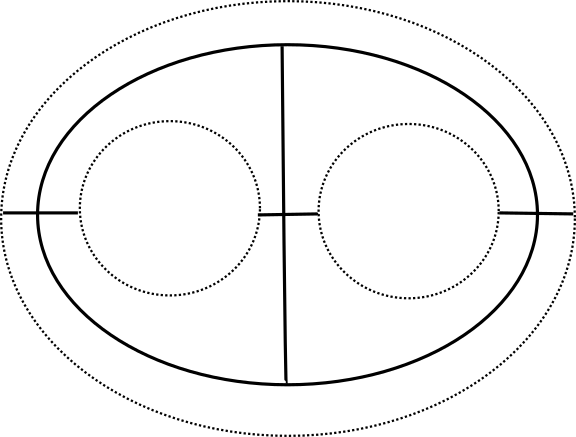
\includegraphics[scale=0.3]{3punctured}
\centering
\end{figure}
\end{example}

Following Corollary \ref{lifting_cor}, we have the lifting lemma for $k$-substratal pairs.

\begin{lemma}
\label{substratal_lift}
Let $R\to X$ be a Serre fibration with fiber $F$ $(k-1)$-connected. Then it has the relative lifting property with respect to all $k$-substratal pairs $(Z, A)$:

\begin{equation*}
\begin{tikzcd}
A \arrow[r] \arrow[hookrightarrow]{d}
& R \arrow[d]
\\
Z \arrow[r] \arrow[dashed,ur,"\exists"]
& X.
\end{tikzcd}
\end{equation*}
\end{lemma}

\begin{example}
Consider a $3$-punctured sphere as in the last example. Since it is $1$-substratal, we can solve the lifting problem
\begin{equation*}
\begin{tikzcd}
\emptyset \arrow[r] \arrow[hookrightarrow]{d}
& R \arrow[d]
\\
S^2\setminus\{0,1,\infty\} \arrow[r] \arrow[dashed,ur,"\exists"]
& X
\end{tikzcd}
\end{equation*}
for all Serre fibration $R\to X$ with $0$-connected (i.e. connected) fiber.
\end{example}

Given the results above, we can understand the space of formal solutions, i.e. sections of the partial differential relation $R\to X$, as a lifting problem. Let's look at the space of formal immersions of a $m$-dimensional manifold $X$ into $\R^n$. Let $R^{\Imm} \subset J^1(X,\R^n)$ denote the partial differential relation corresponding to immersions $X\looparrowright \R^n$. Let $F^{\Imm}$ be the fiber of $R^{\Imm}\to X$ over $x \in X$. Then
\begin{equation*}
F^{\Imm} = \R^n \times \Hom^{\mathrm{Inj}}(T_xX,\R^n) \simeq \Hom^{\mathrm{Inj}}(T_xX,\R^n),
\end{equation*}
where $\Hom^{\mathrm{Inj}}(T_xX,\R^n)$ denotes the set of injective homomorphisms. Note that we have identified a tangent space of $\R^n$ with $\R^n$ itself. Fix a basis for $T_xX$ so $\Hom^{\mathrm{Inj}}(T_xX,\R^n) \cong \Hom^{\mathrm{Inj}}(\R^m,\R^n)$. Then $F^{\Imm}$ is homotopically equivalent to $\GL_n(\R)/GL_{n-m}(\R)$ (specifying $m$ linearly independent vectors in $\R^n$). Recall that $\GL_n(\R)$ deformation retracts onto $O(n)$ by Gram-Schmidt process. It follows that
\begin{equation*}
F^{\Imm} \simeq O(n)/O(n-m).
\end{equation*}
We now want to know the connectedness of $F^{\Imm}$. The key observation is the following fibration
\begin{equation*}
O(k)\to O(k+1) \to O(k+1)/O(k) \cong S^k.
\end{equation*}
Recall that $\pi_i(S^k) = 0$ for all $i <k$ and $\pi_k(S^k) = \Z$. Combining this with the homotopy exact sequence, we have
\begin{equation*}
\pi_k O(k) \to \pi_k O(k+1)
\end{equation*}
is surjective and
\begin{equation*}
\pi_i O(k) \to \pi_i O(k+1)
\end{equation*}
is isomorphic for all $i < k$.

Now $F^{\Imm}$ fits into the fibration
\begin{equation*}
O(n-m)\to O(n) \to O(n)/O(n-m) \simeq F^{\Imm}.
\end{equation*}
The key fact above shows that
\begin{equation*}
\pi_{n-m-1}O(n-m)\to\pi_{n-m-1}O(n)
\end{equation*}
is surjective and
\begin{equation*}
\pi_{i}O(n-m)\to\pi_{i}O(n)
\end{equation*}
is isomorphic for $i < n-m-1$. Thus from homotopy exact sequence we have
\begin{equation*}
\pi_iF^{\Imm} = 0
\end{equation*}
for $i \le n-m-1$. Assume $n=2m$. So $F^{\Imm}$ is $(m-1)$-connected. Since $X$ is an $m$-manifold, it is $m$-substratal. By Lemma \ref{substratal_lift}, it follows a formal solution to the immersion problem exists. This is not too satisfying, because we already knew a genuine solution exists.

Assume now that $X$ is $(m-1)$-substratal obtained from an $(m-1)$-complex $A \subset X$. This includes many cases when $X$ is noncompact. Consider the pair $(X\times I, X\times \partial I)$. Then $X\times I$ can be obtained from $X\times\partial I$ by gluing acyclic cells (think of the case when $X=\R$ and $A$ is a point). So $(X\times I, X\times \partial I)$ is $m$-substratal.

\begin{theorem}
$\Imm(X,\R^n)$ satisfies the $0$-parametric h-principle provided that $n=2\dim X$ and $X$ is $(m-1)$-substratal. In other words, every formal solution is homotopic to a genuine solution.
\end{theorem}

\begin{proof}
Since the pair $(X\times I, X\times \partial I)$ is $m$-substratal, we can solve the lifting problem
\begin{equation*}
\begin{tikzcd}
X\times\partial I \arrow[r] \arrow[hookrightarrow]{d}
& R \arrow[d]
\\
X \times I \arrow[r] \arrow[dashed,ur]
& X
\end{tikzcd}
\end{equation*}
This shows that the space of formal solutions, i.e. sections of the bundle $R \to X$, is connected.  Since a genuine solution is a formal solution, and there are genuine solutions by Corollary \ref{thm:jettransimm}, this implies that there is a path from any formal solution to any genuine solution, going through formal solutions.
\end{proof}
Note that this does not show that the space of genuine solutions is connected. Here the condition being $k$-substratal is rather superficial. Later on we will introduce more powerful methods to remove this condition.

\marginnote{\textbf{2-16-18}}

We would like to finish understanding $R^{\Morse}$. We first recall the notion of a pushout.

\begin{definition}
Given maps $i: B \to A$, $j: B \to C$, the \emph{pushout} of $i$ and $j$ consists of a space, denoted $A \cup_B C$, and maps $A \to A\cup_B C$, $C \to A\cup_B C$ satisfying the property that, for any space $Z$ and maps $A \to Z$, $C \to Z$ making the following diagram commute:
\begin{equation*}
\begin{tikzcd}
B \arrow[r, "j"] \arrow[d,"i"] & C \arrow[d] \arrow[ddr, bend left=10] \\
A \arrow[r] \arrow[drr, bend right=10] & A \cup_B C \arrow[dashed, "\exists!", dr] \\
& & Z
\end{tikzcd}
\end{equation*}
there exists a unique map $A \cup_B C \to Z$ which again makes the diagram commute.
\end{definition}

An important property of the pushout is that it is not homotopy invariant; that is, there exist spaces fitting into the commutative diagram
\begin{equation*}
\begin{tikzcd}
A \arrow[d,swap, "\simeq"] & B \arrow[l, "i"] \arrow[r, "j"] \arrow[d, "\simeq"]& C \arrow[d, "\simeq"] \\
A' & B' \arrow[l,swap, "i'"] \arrow[r, "j'"] & C'
\end{tikzcd}
\end{equation*}
such that $A \cup_B C \not\simeq A' \cup_{B'} C'$. Consider the following examples.
\begin{example}
The following two diagrams are pushout diagrams.
\begin{equation*}
\begin{tikzcd}
S^1 \arrow[r,hook] \arrow[d,hook] \arrow[dr, phantom, "\ulcorner", very near start] & D^2 \arrow[d] \\
D^2 \arrow[r] & D^2 \cup_{S^1} D^2 \approx S^1
\end{tikzcd} \qquad
\begin{tikzcd}
S^1 \arrow[r,hook] \arrow[d,hook] \arrow[dr, phantom, "\ulcorner", very near start] & pt \arrow[d] \\
pt \arrow[r]& D^2 \cup_{S^1} D^2 \approx pt
\end{tikzcd}
\end{equation*}
However, $S^1 \not\simeq pt$. 
\end{example}

For this reason, we will instead consider the notion of a \emph{homotopy pushout}.

\begin{definition}
Given maps $i : B \to A$, $j: B \to C$, the \emph{homotopy pushout} of $i$ and $j$ consists of a space, denoted by either $A \cup_B^H C$ (or more simply by $M(i,j)$), and maps $A \to A \cup_B^H C$, $C \to A \cup_B^H C$ satisfying the property that, for any space $Z$ and maps $A \to Z$, $C \to Z$ making the following diagram commute:
\begin{equation*}
\begin{tikzcd}
B \arrow[r, "j"] \arrow[d,"i"] & C \arrow[d] \arrow[ddr, bend left=10] \\
A \arrow[r] \arrow[drr, bend right=10] & A \cup_B C \arrow[dashed, "\simeq", dr] \\
& & Z
\end{tikzcd}
\end{equation*}
there exists a map $A \cup_B C \to Z$ which makes the diagram commute up to homotopy.
\end{definition}

We note that $M(i,j)$ can be constructed explicitly by taking
\begin{equation*}
M(i,j) = A \cup_{B \times \{0\}} (B \times [0,1]) \cup_{B \times \{1\}} C.
\end{equation*}
We will soon show that the homotopy pushout is homotopy invariant. But first, we revisit the previous example. 

\begin{example}
For the maps $i,j: S^1 \hookrightarrow D^2$, we have
\begin{align*}
M(i,j) &= D^2 \cup_{S^1 \times \{0\}} (S^1 \times [0,1]) \cup_{S^1 \times \{1\}} D^2 \\
&\cong S^2,
\end{align*}

and for the maps $i', j': S^1 \to pt$, we have
\begin{align*}
M(i',j') &= pt \cup_{S^1 \times \{0\}} (S^1 \times [0,1]) \cup_{S^1 \times \{1\}} pt \\
&\cong S^2.
\end{align*}
So, in this case, the homotopy pushout is homotopy invariant. 
\end{example}

We now show that this is always the case.

\begin{lemma}\label{hompoinvar}
The homotopy pushout is homotopy invariant, i.e., if there is a commutative diagram
\begin{equation*}
\begin{tikzcd}
A \arrow[d,swap, "\simeq"] & B \arrow[l, "i"] \arrow[r, "j"] \arrow[d, "\simeq"]& C \arrow[d, "\simeq"] \\
A' & B' \arrow[l,swap, "i'"] \arrow[r, "j'"] & C'
\end{tikzcd}
\end{equation*}
then the map $M(i,j) \to M(i',j')$ is a homotopy equivalence. 
\end{lemma}

\begin{proof}
Let 
\begin{align*}
U &= A \cup_{B \times \{0\}} (B \times [0,1)) \simeq A\\
V &= (B \times (0,1]) \cup_{B \times\{1\}} C \simeq C,
\end{align*}
and similarly define $U', V'$. Then $U \cap V \cong B \times (0,1) \simeq B$ and $U' \cap V' \simeq B'$. These spaces fit into the commutative diagram
\begin{equation*}
\begin{tikzcd}
U \arrow[d, "\simeq"] & U \cap V \arrow[l, hook'] \arrow[r, hook] \arrow[d, "\simeq"] & V \arrow[d, "\simeq"] \\
U' & U' \cap V' \arrow[l, hook'] \arrow[r,hook] & V'
\end{tikzcd}
\end{equation*}
So, the map $M(i,j) = U \cup V \to U' \cup V' = M(i',j')$ is a homotopy equivalence.
\end{proof}

\begin{example}[Join of Spaces]
Consider the case of a Cartesian product $X \times Y$ with projections $p_1: X \times Y \to X$ and $p_2: X \times Y \to Y$. Then $M(p_1, p_2)$ is called the \emph{join} of $X$ and $Y$, and is denoted $X \star Y$. 
\end{example}

\begin{example}
The join of two intervals, $[0,1] \star [0,1]$ is homeomorphic to a $3$-simplex. 
\begin{figure}[h]
\centering
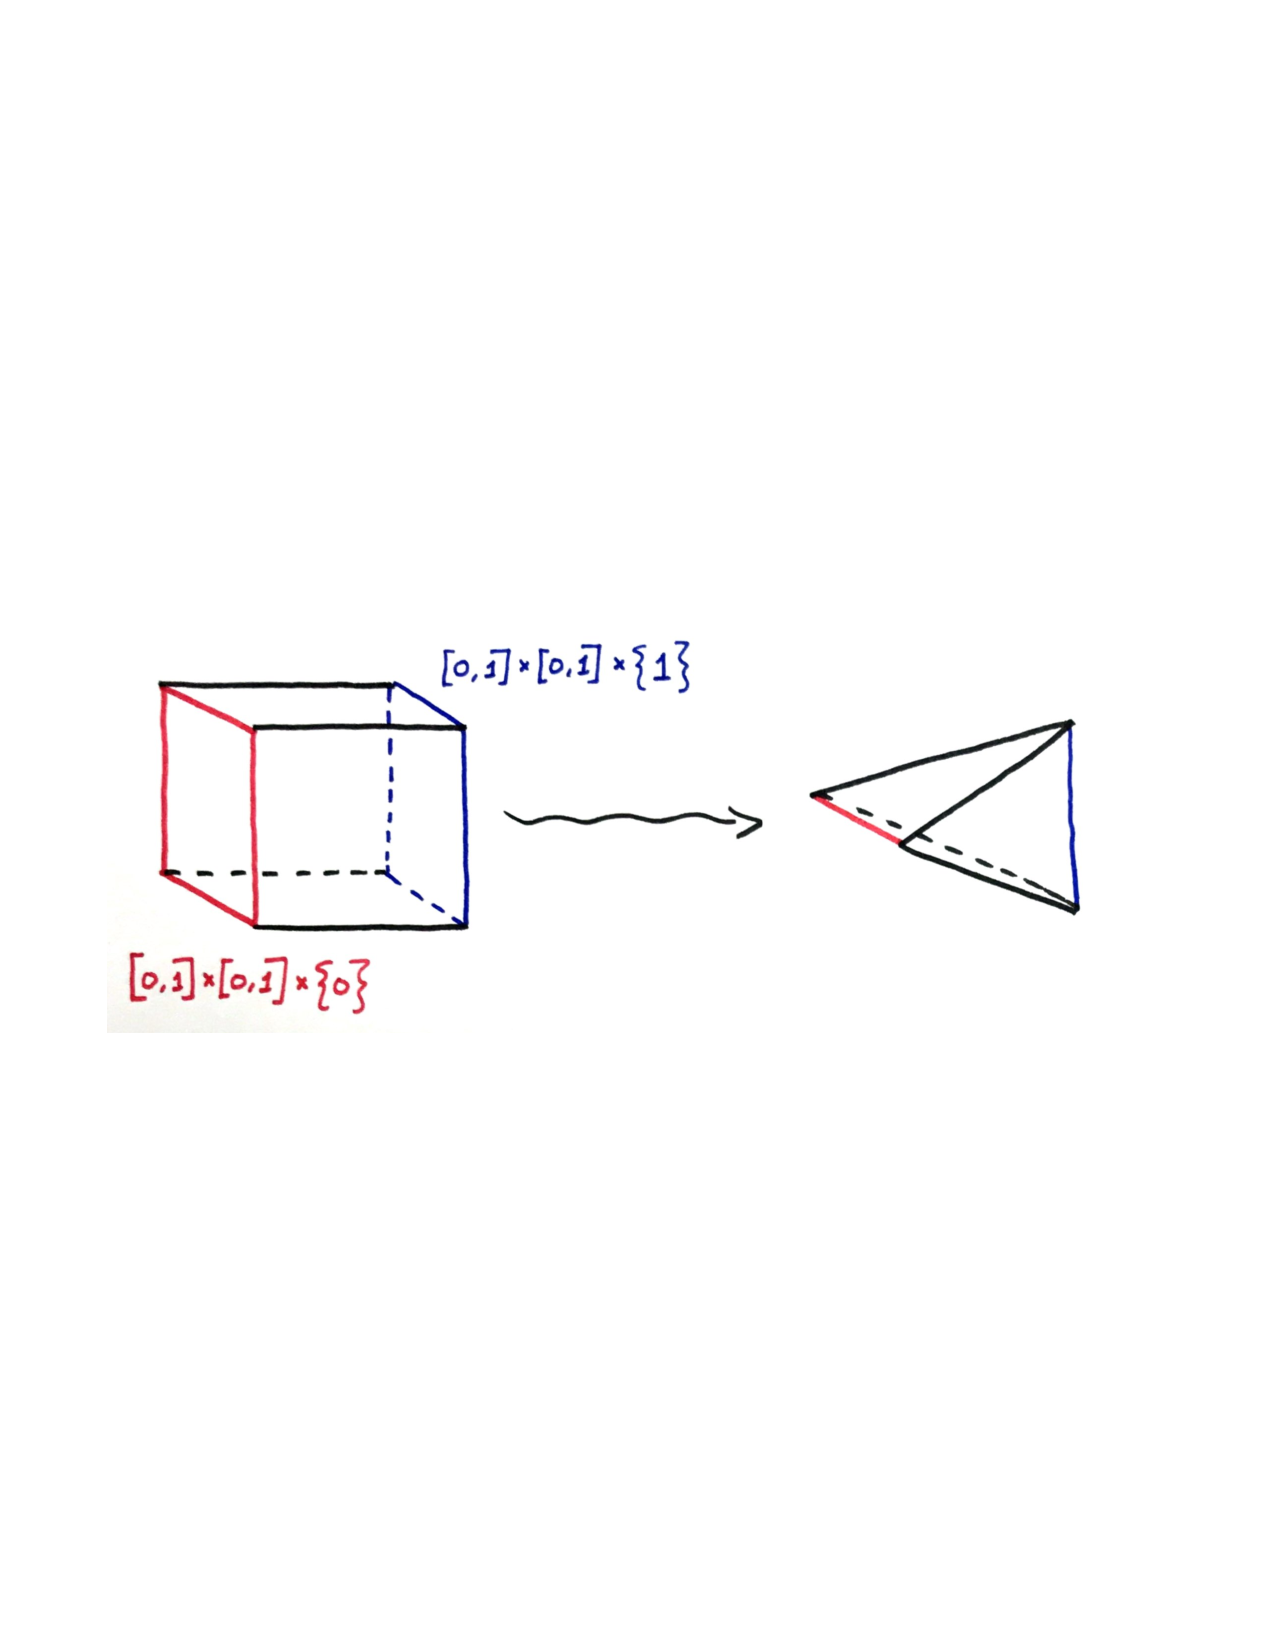
\includegraphics[width=8cm]{joinint}
\caption{The join of two intervals is a $3$-simplex}
\end{figure}
\end{example}

\begin{example}
\begin{enumerate}[(i)]
\item $X \star pt \cong C(X)$, the cone on $X$.
\item $X \star S^0 \cong S(X)$, the suspension of $X$.
\item $S^m \star S^n \cong S^{m+n+1}$
\end{enumerate}
\end{example} 

We now turn our attention the fiber bundle $F^{\Morse} \to R^{\Morse} \to X$. Recall that $R^{\Morse} = S_0^{(2)} \cup S_{1,0}$. Then we have the fibers $F_0^{(2)}$ and $F_{1,0}$ over $S_0^{(2)} \to X$ and $S_{1,0}$, respectively.

\begin{proposition}
If $\dim X = m$, then $F^{\Morse} \simeq S^{m-1} \star \left( \bigsqcup_k \Gr_k(\mathbb{R}^m) \right)$.
\end{proposition}

\begin{proof}
Recall that by the Spectral Decomposition Theorem $F_{1,0} \simeq \bigsqcup_k \Gr_k(T_x X)$. So, it suffices to show that $F^{\Morse} \simeq S^{m-1} \star F_{1,0}$. 

Let $U = F_0{(2)} =  \{ \text{jets with } df_x \neq 0\} \simeq S^{m-1}$ (this deformation retracts onto the sphere bundle $S(T_x^* X)$). Since we only care about the homotopy type of $F^{\Morse}$ and $X$ is locally Euclidean, we can assume $X = \mathbb{R}^m$. Then, after choosing coordinates, we can define $V = \{ \text{jets with non-deg Hessian} \} \simeq F_{1,0}$.  Then $U \cup V = F^{\Morse}$ and $U \cap V \simeq F_{1,0} \times \left( T_x^* X \setminus 0 \right) \simeq F_{1,0} \times S^{m-1}$. This is summarized in the following commutative diagram.
\begin{equation*}
\begin{tikzcd}
S^{m-1} \arrow[d, "\simeq"] & F_{1,0} \times S^{m-1} \arrow[l,swap, "p_2"] \arrow[r, "p_1"] \arrow[d, "\simeq"] & F_{1,0} \arrow[d, "\simeq"] \\
U & U \cap V \arrow[l, hook'] \arrow[r, hook] & V
\end{tikzcd}
\end{equation*}
Thus, by Lemma \ref{hompoinvar}, 
\begin{equation*}
F^{\Morse} = U \cup V \simeq U \cup_{U \cap V}^H V \simeq F_{1,0} \cup_{F_{1,0} \times S^{m-1}}^H S^{m-1} \simeq F_{1,0} \star S^{m-1},
\end{equation*}
and so we are done.
\end{proof}

This proposition along with the Freudenthal Suspension Theorem \cite{may1999concise} immediately gives the following corollary.

\begin{corollary}
If $\dim X = m$, then $F^{\Morse}$ is $(m-1)$-connected.
\end{corollary}

\begin{proposition}
If $X$ is $(m-1)$-substratal, the the space of formal solution to $R^{\Morse}$ is connected.
\end{proposition}

\begin{proof}
Proposition from 2-14-18 (not added yet).
\end{proof}

\begin{corollary}
Morse functions satisfy the $0$-parametric $h$-principle on $X$, provided that $X$ is $(m-1)$-substratal.
\end{corollary}



\marginnote{\textbf{2-19-18}}

\section{Morse functions and Generalized Morse functions}

Given a smooth manifold M and a smooth function $f\colon M \to \mathbb{R},$

\begin{lemma}
If $p_0$ is a critical point of f then;
 \begin{align*} 
Hess(f)_{p_0}&\colon T_{p_0}M\times T_{p_0}M\to \mathbb{R} \\
&(v,w)\mapsto \tilde{v}_{p_0}(\tilde{w}(f)), \\
&\text{(where $\tilde{v}$ and $\tilde{w}$ are smooth vector fields on M that evaluate at $p_0$ to v and w respectively)}
\end{align*}
is a well-defined symmetric bilinear map.
\end{lemma}
\begin{proof}


 $p_0\in Crit(f)$, i.e. $df_{p_0}\equiv 0,$ so we get 
\begin{align*}
df_{p_0}([\tilde{v},\tilde{w}])&=0\\
(\tilde{v}\tilde{w}-\tilde{w}\tilde{v})_{p_0}(f)&=0\\
\tilde{v}_{p_0}(\tilde{w}(f))&=\tilde{w}_{p_0}(\tilde{v}(f))\hspace{4mm} \text{(Note: The left hand-side of this equation is, by definition, $Hess(f)_{p_0}(v,w)$)}\\
v(\tilde{w}(f))&=w(\tilde{v}(f)) \hspace{7mm} (\text{follows since $\tilde{v}_{p_0}=v$ and $\tilde{w}_{p_0}=w$})
\end{align*}
Now observe that the left hand-side of the last line does not depend on $\tilde{v}$ and the right hand-side does not depend on $\tilde{w},$ so we get well-definedness and symmetry at the same time by realizing that the right hand-side of the last equation is $Hess(f)_{p_0}(w,v).$ Bilinearity just follows from the fact that vectors act linearly on functions. 
\end{proof}

\underline{Recall}:\newline
1) $Hess(f)_{p_0}$ can be represented locally in coordinates $x=(x^1,...,x^n)$ centered at $p_0$ by the matrix $$\Big[\frac{\partial^2 f(x)}{\partial x^i \partial x^j}\Big|_{x=p_0}\Big]$$ and is said to be "non-degenerate" if this matrix is non-singular (at critical points, non-degeneracy is coordinate independent by the coordinate independence of the Hessian map itself, which we have demonstrated above).\newline
2) Morse Critical points have non-degenerate Hessians.
\newline
\newline
For generalized Morse functions, we allow critical points where the Hessian is degenerate, but only co-rank 1. (i.e. $rank(Hess(f)_{p_o})=dimM-1$). For such critical points we have a distinguished direction, $X\in Ker(Hess(f)_{p_0})\backslash \{0\}$ points in this direction.
\newline
\newline
$\underline{Observation}:$ 
$$XYf(p_0)=0\hspace{4mm} \forall \hspace{2mm}Y\in T_{p_0}M$$
But from the lemma, we know $XYf(p_0)=YXf(p_0)$
Therefore $p_0$ is also a critical point of the map $g:=(p\mapsto \tilde{X}_pf \hspace{3mm}\forall p\in M)$ where $\tilde{X}$ is any extension of $X$ to a smooth vector field on M. So by the lemma we started with, the Hessian of g is well-defined at $p_0.$
So we can define the map \newline
$(sX\mapsto s^3Hess(g)_{p_0}(X,X)\hspace{3mm} \forall s\in \mathbb{R})$ \hspace{4mm}(This can be thought of as a cubic form on $span(X)$)
For a generalized Morse function, we require that this map is not the zero map.
\newline
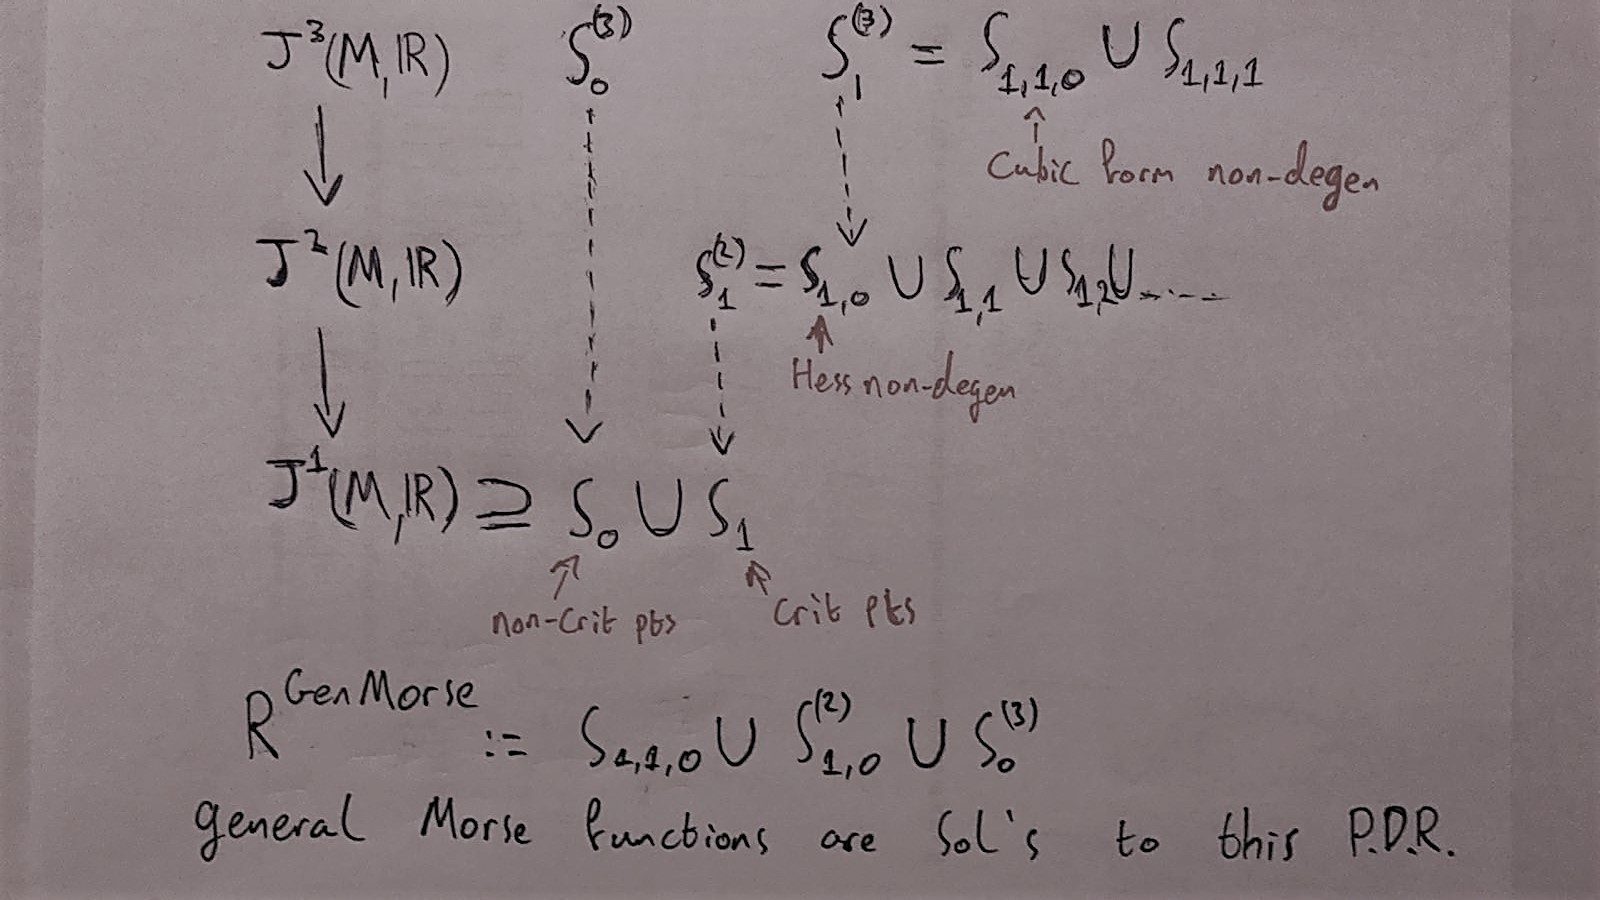
\includegraphics[width=8cm]{GeneralMorse.jpg}

The jet transversality theorem implies the existence of a function $f:M\mapsto \mathbb{R}$ such that $j^{k}f$ $\pitchfork$ each $S_i,S_{i,j},S_{i,j,k}...$ etc.
\begin{corollary}
For M a smooth manifold, Morse functions exist! 
\end{corollary} 
Apply Jet transversality to paths of functions $M\times I\to \mathbb{R}.$
\newline
$\underline{Question}:$
Is the space of Morse functions connected?
The answer is no because of the involvement of higher codimension singularities (namely $S_{1,1,0}$)
\newline
\newline
\begin{equation*}
\begin{tikzcd}
j^3f^{-1}(S_{1,1,0}) \arrow[r] \arrow[d] \arrow[dr, phantom, , very near start]
& S_{1,1,0}   
 [d] \arrow[d, phantom,"\big| \bigcap" , near start] \\
X\times I \arrow[r]
& J^3(X,\mathbb{R})
\end{tikzcd}
\end{equation*}
\newline
\newline
\begin{align*}
j^3f^{-1}(S_{1,1,0})&=\text{paths in $X\times I$ where we have an $S_{1,1,0}-singularity$}\\ 
S_{1,1,0}(f)&=\{\hspace{1mm}(m,t)\in M\times I \hspace{3mm}|\hspace{3mm} j^3f_t(m_0)\in S_{1,1,0}\hspace{1mm}\}
\end{align*}
\newline
\newline
If M is compact, this is a finite zero dimensional submanifold of $M\times I$.

\begin{corollary}
Any two Morse functions are connected by a path of functions which are Morse for all but finitely many values of time, the times where we have an $S_{1,1,0}$ singularity.
\end{corollary}
$\underline{\textbf{MORSE LEMMA:}}$
If $f\colon M \to \mathbb{R}$ is smooth, $p_0$ a Morse critical point then there exists a coordinate system $(U,x)$ centered at $p_0$ such that;
$$f|_{U}=f(p_0)-\sum_{i=1}^{k}(x^i)^2+\sum_{i=k+1}^{m}(x^i)^2$$
where, k:= index of f at $p_0$ which is defined to be the maximal dimension of a subspace of $T_{p_0}M$ on which the hessian of f at $p_0$ is negative definite. 
\newline
Note: This implies that non-degenerate critical points are isolated. 
\newline
\newline
\underline{Corresponding lemma for $S_{1,1,0}$ singularities}:


$$f|_{U}=f(p_0)+(x^1)^3-\sum_{i=2}^{k}(x^i)^2+\sum_{i=k+1}^{m}(x^i)^2.$$

\marginnote{\textbf{2-21-18}}

We refocus our attention to the Morse differential relation $R=S^{(2)}_0 \cup S_{1,0} \subset J^2(X,\R)$ and its genuine solutions.  As it was for immersions, it turns out that the space of genuine solutions is not connected.  But in the case of Morse functions, we can do something close.  To do this we will need to allow for functions that have nondegenerate Hessians in our paths of functions. Thus we recall the definition of the higher analogues of the Hessian.

The Hessian of a function $f \in C^\infty(X)$ at a critical point $p \in X$ has the following coordinate invariant description.  It is a billinear form defined by sending the vectors $\xi_1, \xi_2 \in T_pX$ to $\Xi_1(\Xi_2(f))(p)$ where $\Xi_i$ is an extension of $\xi_i$ to a vector field on $X$.  One can check that this doesn't depend on the choice of extension of the vector fields, precisely because $p$ is a critical point, i.e. $\xi$ is in the null space of $df_p$.  One could have also defined the quadratic form by sending a single vector $\xi \in T_pX$ to $\Xi(\Xi(f))_p$.

If this billinear form is of corank 1, then one can define a cubic form on a one dimensional vector space, namely the null space of the Hessian.  The form sends $\xi$ to $\Xi(\Xi(\Xi(f)))$.  If this form is nondegenerate, (since the form is one dimensional this just means that the form is nonzero), then we say that $j^3f(p) \in S_{1,1,0}\subset J^3(X,\R)$.  This defines the stratum $S_{1,1,0} \subset J^3(X,\R)$.   \footnote{ For more information about these so called "Thom-Boardman Strata", and definitions of $S_{1,j,k}$ etc, see page 156 of \cite{strata}}

\begin{definition}
The generalized morse function $f \in C^\infty(X)$ is a function taking $S_0$, $S_{1,0}$ or $S_{1,1,0}$ singularities.  i.e. these are the $f$ such that at any $p$, $j^1f \in S_0$, $j^2f(p) \in S_{1,0}$, or $j^3f(p) \in S_{1,1,0}$.
\end{definition}

Morse functions have a nice local coordinate description, and generalized morse functions have a similar local coordinate description:

\begin{fact}[Morse Lemma]

If $p$ is a $S_{1,0}$ singularity of $f$, then there are coordinates $(x_1,...x_n)$ centered at $p$, such that $f(x_1....x_n)=f(p)+ \sum_{i=1}^{n-k} x_i^2- \sum_{j=n-k+1}^m x_j^2$.  $k$ is called the index of the critical point $p$.

\begin{proof}
See \cite{strata} page 65 or Milnor's Morse Theory.
\end{proof}
\end{fact}

\begin{fact}[Generalized Morse Lemma]
If $p$ is a $S_{1,1,0}$ singularity then there are coordinates $(x_1,...x_n)$ centered at $p$ such that $f(x_1,...x_n)=f(p)+x_1^3+\sum_{i=2}^{m-k} x_i^2 -\sum_{j=m-k+1}^m x_j^2$.
\begin{proof}
See \cite{strata} page 177.  
\end{proof}

\end{fact}

The space of Morse functions is not path connected:  Let $X$ be any space that admits two morse functions that have different number of critical points.  One can take $X=S_1$ and $f$ given by two different height functions for instance.  It is a good exercise to prove using \ref{thm: thomJT} that for any homotopy $h_t$ such that $h_t$ is a Morse function for each time, $h_t$ has the same number of critical points (and in fact has the same number of critical points of a given index).

The following example illustrates what happens when trying to connect two Morse functions with differing number of critical points.  
\begin{example}
Consider the homotopy $h_t(x)=x^3+tx$.  \[d(h_t)=3x^2+t\]
The critical points are  $x=\pm  \sqrt{-t/3}$ when $t<0$ of index 1 and -1 respectively,  a critical point with degenerate Hessian at $x=0$ at $t=0$ and there are no critical points for $t>0$.  $h_t$ is a Morse function when $t \neq 0$.  One can read off the indexes /degeneracies of the critical points from the shape of the graph (you can look to see if around the critical point $f$ looks locally like parabola, upside down parabola,... or in higher dimensions you can look to see if $f$ looks like a paraboloid, a hyperbolic saddle or an upside down parabola), or from direct computation.  Note that in the transition between $t<0$ and $t>0$, 2 critical points had to "die".  This intuitively explains why one cannot connect two arbitrary Morse functions through Morse functions. For more information on birth or death critical points, see Igusa's paper on $C_1$ local parametrized Morse Theory.

\end{example}

We will now show that arbitrary Morse functions can be connected through generalized Morse functions, and we will prove it using observation \ref{thm: transverse} and the Thom transversality theorem (\ref{thm: thomJT}).  Take the map $J^2(M \times I, \R) \xrightarrow{\pi}  J^2(M,\R)$ induced from the map $M \times I  \to M$. For any $R \subset J^(M, \R)$, we can consider the relation $\pi^{-1}(R) \subset J^2(M \times I, \R)$.  For instance we could take $\pi^{-1}( S_{1,0}) \subset J^2(M \times I, \R)$.  Note that for a homotopy $h: M \times I \to \R$, $j^2 h \in \pi^{-1}(S_{1,0}) \iff j^2(h_t)(x) \in S_{1,0}$.  An analagous statement holds for an arbitrary relation $R$. Thus a homotopy through a generalized morse function is a $h \in C^\infty(M \times I)$ such that for all $p$,  $j^2 h(p) \notin \pi^{-1}(S_{1,i})$ $\forall i>1$, and $j^3 h(p) \notin \pi^{-1}(S_{1,1,i}) \forall i>0$.

One can compute in a method analagous to \ref{howcomputedimension} that 
\[codim (\pi^{-1}(S_{0}))=0 \]
\[codim (\pi^{-1}(S_{1,0}))=dim M \]
\[codim (\pi^{-1}(S_{1,1,0}))=dim M+1=dim(M \times I) \]
 
And the codimension of the spaces
$\pi^{-1}(S_{1,i}) i>1$, and $ \pi^{-1}(S_{1,1,i}) i>0$ is greater than $dim(M \times I)$.  Jet transversality implies that for generic $h$ $j^1h, j^2h, j^3h$ are transverse to all of these spaces.   $j^2h$, $j^3h$ being transverse to the spaces $\pi^{-1}(S_{1,i}) i>1$, and $ \pi^{-1}(S_{1,1,i}) i>0$  implies by part $(i)$ of \ref{thm: transverse}, that $j^2 h(p) \notin \pi^{-1}(S_{1,i})$ $\forall i>1$, and $j^3 h(p) \notin \pi^{-1}(S_{1,1,i}) \forall i>0$ - i.e that $h_t$ is a generalized Morse function for all $t$.   Moreover $j^2(h(x,t))$ transverse to $\pi^{-1}(S_{1,1,0})$ implies by part $(ii)$ of  \ref{thm: transverse} that $j^2(h(x,t))$ only intersects $\pi^{-1}(S_{1,1,0})$ in a discrete set.  Thus $j^2(h_t)$ only intersects $S_{1,1,0}$ for finitely many $t$.

\subsection{(Lecture on 2/23) Fibers of generalized Morse PDR}
A generalized Morse PDR breaks down as:
$$ R^{gMorse}=S_0^{(3)}\cup S_{1,0}^{(3)}\cup S_{1,1,0}\subseteq J^3(M, \mathbb{R})$$

We now want to look at the fiber $F^{gMorse}$ of $R^{gMorse}\to M$. We have the following maps:
\begin{equation*}
\begin{tikzcd}
J^3(M,\R)\arrow[d]\\
J^2(M,\R)\arrow[d]\\
J^1(M,\R)\arrow[d]\\
J^0(M,\R)=M\times \R
\end{tikzcd}
\end{equation*}

We now look at the different parts of the decomposition of the fiber. We have that $F_{1,0}\cong \bigsqcup\limits_{k \text{index}} Gr_k(\R^m)=\bigsqcup\limits_{k}O(m)/(O(k)\times O(m-k))$. This gives us a spectral decomposition of the Hessian; i.e. a configuration space of points in $\R$ which satisfy three conditions:
\begin{enumerate}
\item $\lambda_i\neq 0$ (non-degeneracy condition)
\item $v_i\perp v_j, \forall i\neq j$
\item $\bigoplus v_i=T_xX$
\end{enumerate}
\begin{center}
\begin{tikzpicture}[dot/.style={circle,inner sep=1pt,fill,label={#1},name=#1},
  extended line/.style={shorten >=-#1,shorten <=-#1},
  extended line/.default=1cm]

\node [dot=$v_1$] at (0,1) {};
\node [dot=$v_2$] at (1,1) {};
\node [dot=$v_3$] at (4,1) {};

\draw[<->] (-1,0) -- (5,0) node[right]{$\R$};

\foreach \x/\testosopra/\testosotto in {0/\lambda_1/, 1/\lambda_2/, 3/0/, 4/\beta/}{
 \draw(\x,0.1)--(\x,-0.1);
 \node[above,font=\scriptsize]at (\x,0.1) (\x) {$\testosopra$};
 \node[below,font=\scriptsize]at (\x,-0.1) {$\testosotto$};
}
\end{tikzpicture}
\end{center}

The $F_{1,1}$ fiber consists of the Hessians with one-dimensional kernel. For $i>1, F_{1,i}$ are the Hessians with kernel of dimension greater than 1. \\

In the third jet space, we get everything above $S_0, S_{1,0}$, and also everything above $S_{1,1,0}$. What are these last fibers? They are 1-dimensional cubic forms on $V_0$: 
$$q:V_0\to \R \text{ such that } q(rx)=r^3q(x)$$
If $q$ is non-degenerate (i.e. $q\neq 0$), then there exists an element $x\in V_0$ with $q(x)=1$. So the non-degenerate cubic forms on $V_0$ are the same as framings of $V_0$ (i.e. a non-zero vector in $V_0$).\\

We can think of these parts of the fiber through the following schematic (but note that this is just a schematic; really this whole thing like over the origin):\\
\begin{center}
%\includegraphics[scale=.5]{fiber01}
\end{center}

What is the homotopy type of $F_{1,0}\cup F_{1,1}$? We know that this fiber is a configuration space of points satisfying the three conditions listed above.\\

\begin{proposition}\label{F10_F11}
$F_{1,0}\cup F_{1,1}$ is homotopy equivalent to the homotopy colimit (iterated homotopy pushout) of the following diagram:\\
\begin{center}
	\begin{tikzcd}
	&\frac{O(m)}{O(0)\times O(1)\times O(m-1)}\arrow[dl]\arrow[dr]&
	& \frac{O(m)}{O(1)\times O(1)\times O(m-2)}\arrow[dl]\arrow[dr]&\cdots\\
	
	\frac{O(m)}{O(0)\times O(m)} & &\frac{O(m)}{O(1)\times O(m-1)}
	&& \frac{O(m)}{O(2)\times O(m-2)}\\
	
		&\cdots \frac{O(m)}{O(m-1)\times O(1)\times O(0)}\arrow[dl]\arrow[dr]&&&\\
	\cdots & &\frac{O(m)}{O(m)\times O(0)}
	\end{tikzcd}
	\end{center}
\end{proposition}

\subsubsection{Homotopy Colimits}
Suppose we have the following diagram:
\begin{center}
\begin{tikzcd}
A\arrow[d]\arrow[r] & C\\
B
\end{tikzcd}
\end{center}

The homotopy colimit of this diagram is the double mapping cylinder: $B\cup A\times I \cup C$. We can see this by considering $U\simeq B\sqcup C$ and $V\cong A\times (0,1)\simeq A$. Then $U\cup V=A\times (0,\frac{1}{2}\cup A\times (-\frac{1}{2},1)\simeq A\sqcup A$.\\

\begin{proposition}
Let $k$ be the dimension of the strictly negative eigenspace. Then $F_{1,0}^{(k+1)}\cup F_{1,1}^{(k)}\cup F_{1,0}^{(k)}$ is homotopy equivalent to the pushout of the following diagram
	\begin{center}
	\begin{tikzcd}
	&\frac{O(m)}{O(k)\times O(1)\times O(m-k-1)}\arrow[dl]\arrow[dr]&\\
	\frac{O(m)}{O(k+1)\times O(m-k-1)} & &\frac{O(m)}{O(k)\times O(m-k)}
	\end{tikzcd}
	\end{center}
\end{proposition}

Sketch of proof: Take $U=F_{1,0}^{(k+1)}\sqcup F_{1,0}^{(k)}$ and $V=\lbrace$all configuration spaces where there exists a unique eigenvalue closest to the origin which has a 1-dimensional eigenspace$\rbrace$. This gives an open cover of $F_{1,0}^{(k+1)}\cup F_{1,1}^{(k)}\cup F_{1,0}^{(k)}$.\\

Notice that: 
\begin{align*}
U &\simeq \frac{O(m)}{O(k+1)\times O(m-k-1)}\sqcup \frac{O(m)}{O(k)\times O(m-k)}\\
V &\simeq \frac{O(m)}{O(k)\times O(1)\times O(m-k-1)}\\
\Rightarrow U\cup V &\simeq \frac{O(m)}{O(k)\times O(1)\times O(m-k-1)}\sqcup \frac{O(m)}{O(k)\times O(1)\times O(m-k-1)}\\
\end{align*}

Claim: there exists a map from the homotopy pushout of the diagram listed in the proposition to $F_{1,0}^{(k+1)}\cup F_{1,1}^{(k)}\cup F_{1,0}^{(k)}$, which is compatible with the open cover listed above. 


\begin{proposition}
$F^{gMorse}$ is homotopy equivalent to the join of $S^{m-1}$ with  the homotopy colimit of:\\
\begin{center}
	\begin{tikzcd}
	&\frac{O(m)}{O(0)\times O(m-1)}\arrow[dl]\arrow[dr]&
	& \frac{O(m)}{O(1)\times O(m-2)}\arrow[dl]\arrow[dr]&\cdots\\
	
	\frac{O(m)}{O(0)\times O(m)} & &\frac{O(m)}{O(1)\times O(m-1)}
	&& \frac{O(m)}{O(2)\times O(m-2)}\\
	
		&\cdots \frac{O(m)}{O(m-1)\times O(0)}\arrow[dl]\arrow[dr]&&&\\
	\cdots & &\frac{O(m)}{O(m)\times O(0)}
	\end{tikzcd}
	\end{center}
\end{proposition}
This follows from Proposition \ref{F10_F11} above, and the fact that $V_0$ sits as a linebundle over $\frac{O(m)}{O(k)\times O(1)\times O(m-k-1)}$ corresponding to $O(1)$ with framembundle, $Fr(V_0)=\frac{O(m)}{O(k)\times O(m-k-1)}$. The sphere comes from $F_{1,0}^{(3)}\cup F_{1,1,0}$, and can be viewed as the unit sphere of $T_x^*M$.

We see that the homotopy colimit of the diagram directly above is connected, and therefore we get the following:
\begin{corollary}
The fiber of $R^{gMorse}\to M$ is $m$-connected.
\end{corollary}
and therefore by Lemma \ref{substratal_lift} we get
\begin{corollary}
The map $R^{gMorse}\to M$ has the right lifting property for all pairs $(Z,A)$ $(m+1)$-substratal.
\end{corollary}
In particular this implies that it has the lifting property with respect to $(M,\emptyset)$, and $\big((M\times I),(M\times \partial I) \big)$. The latter implies that any two sections of $R^{gMorse}$ are connected, due to the following diagram:
\xymat{M\times \partial I \ar[r]^{\alpha \sqcup \beta} \ar[d] & R^{gMorse}  \ar[d] \\
M\times I \ar[r]_\pi \ar@{-->}[ur]^{\exists}& M}
By letting $M\times \partial I=M\sqcup M$, $\alpha$ and $\beta$ any two sections, and $\pi$ the projection.

\subsection{Morse functions and Handle decomposition}
Why did we in the previous section spend a lot of energy specifically on Morse functions? Not only is this an interesting example in its own right, it will also help us to prove the $h$-principle in other cases. Assume we have a sheaf of interest $\CF$, and an object we are interested in $X$, with a decomposition $X=U\cup V$, then $\CF (X)$ can be recovered from $\CF (U)$, $\CF (V)$, and $\CF (U\cap V)$ by a pullback diagram. Our approach was then to construct a new sheaf $\CF^h$ with a map $\alpha: \CF\to \CF^h$, which was homotopically easier, and we wish to show that $\CF(X)\simeq \CF^h(X)$. Well by studying the following cube:
\xymat{\CF(X) \ar[rr] \ar[dd] \ar[dr]^{\alpha_X} && \CF(U) \ar[dd]|\hole \ar[dr]^{\alpha_U} & \\
&\CF^h(X) \ar[rr] \ar[dd] && \CF^h(U) \ar[dd] \\
\CF(X) \ar[rr]|\hole \ar[dr]^{\alpha_V} && \CF(U\cap V)  \ar[dr]^{\alpha_{U\cap V}} & \\
&\CF^h(X) \ar[rr] && \CF^h(U\cap V)   }
Now if we can show that $\alpha_U$, $\alpha_{V}$, and $\alpha_{U\cup V}$ are weak equivalences, then since the front and the back square are pullbacks it follows that $\alpha_X$ is a weak equivalence. So our goal is to be able to subdivide our manifolds in to parts that play well with our various sheafs of interests, and here handle decomposition will be our primary tool

We here follow \cite{milnor2016morse}, an actual complete treatment of the subject can be found there.
\subsubsection{Handle Decomposition}
For all $0\leq k \leq m$, we have a homeomorphism $D^m\cong D^k\times D^{m-k}$, that gives a description of the boundary as $\partial D^m = \partial(D^k) \times D^{m-k} \cup D^k\times \partial(D^{m-k})$, we call the $\partial(D^k) \times D^{m-k}$-part the base of the $(k-)$handle. 

Let $M$ be a $m$ manifold, potentially with boundary. Given a smooth map from the base of a $k$-handle to $\partial M$, $f:\partial(D^k) \times D^{m-k}\to \partial M\subset M$, we can take the pushout of the diagram
\xymat{\partial(D^k) \times D^{m-k} \ar[r]^f \ar@{^{(}->}[d] & M \\ D^k\times D^{m-k} &}
This might give us a manifold with corners. We smooth out all corners to give us a new $m$-manifold, $M'$, potentially with boundary. 
\begin{figure}[h]
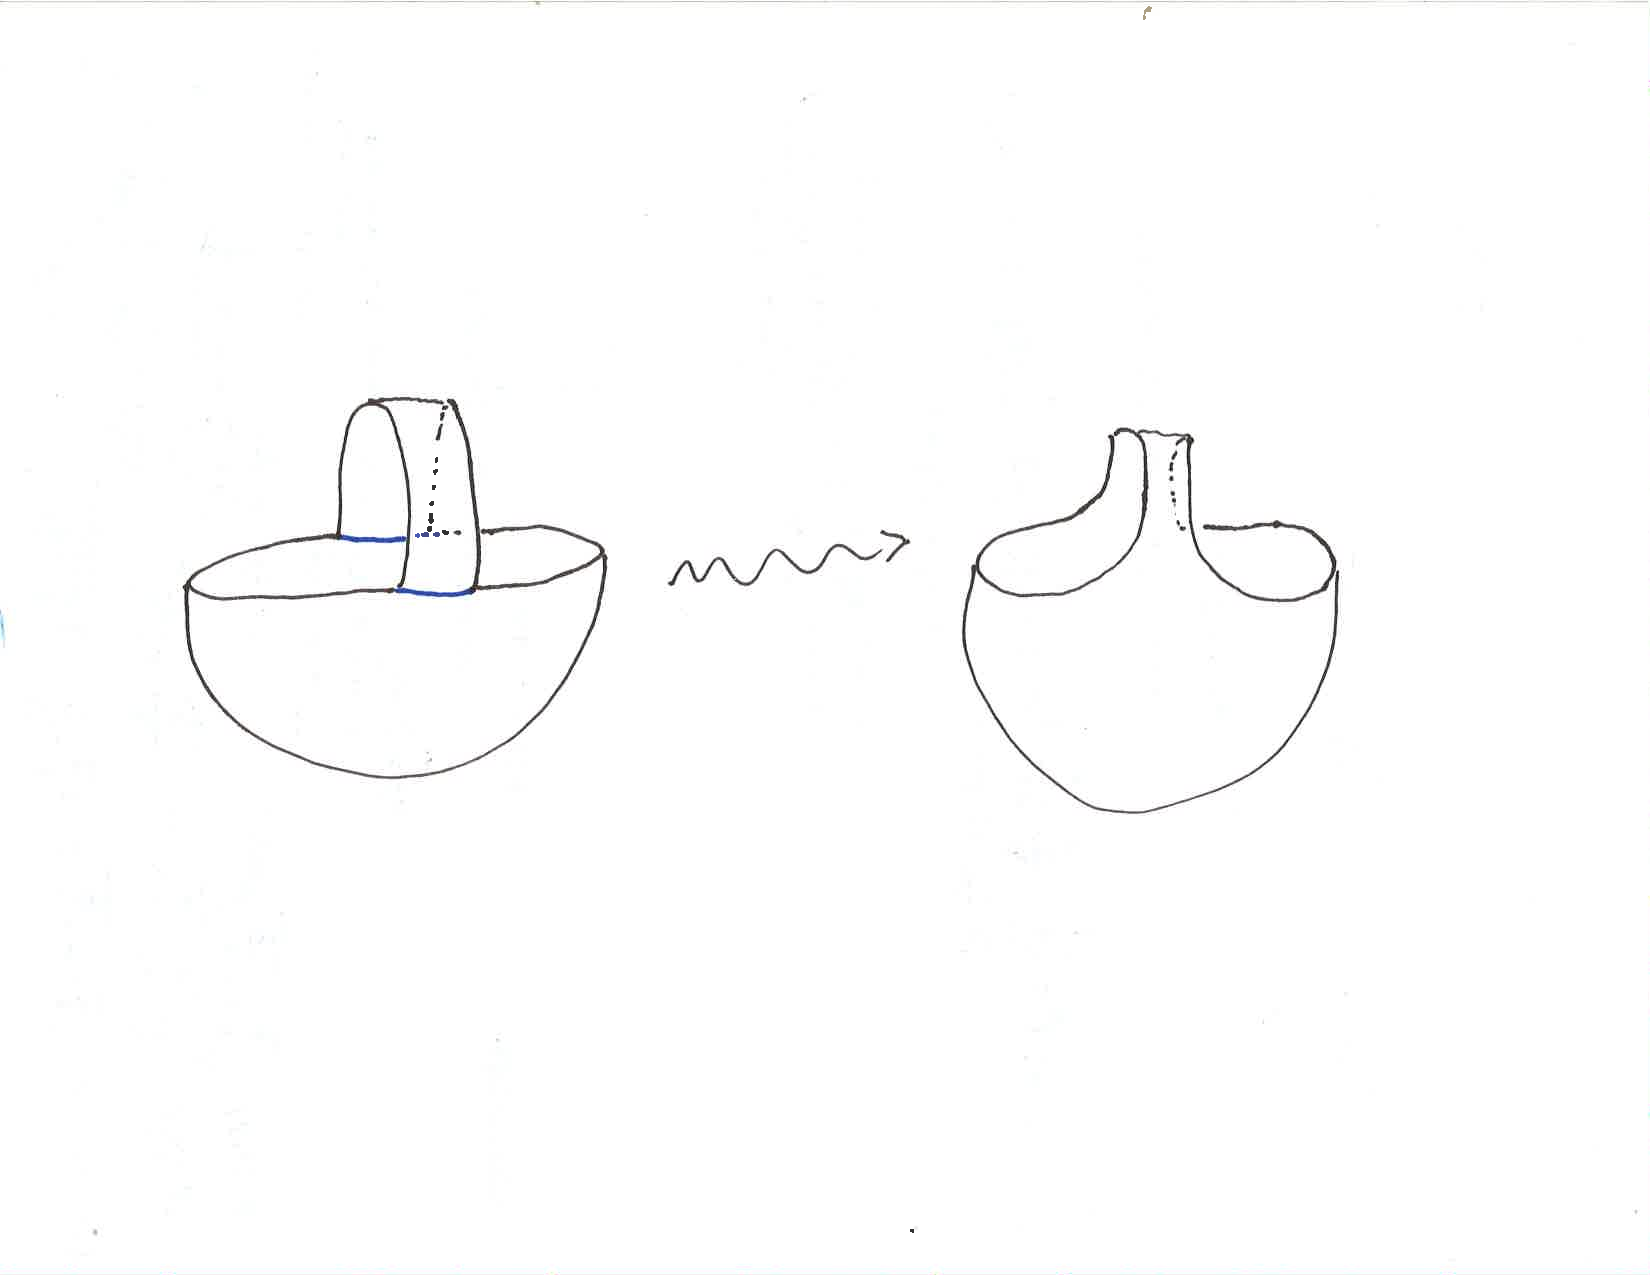
\includegraphics[width=8cm]{attach1handle.pdf}
\caption{Attaching a 1-handle to a 2-disk along the blue line, and then smoothing corners\label{attach1handle}}
\end{figure}
We say that $M'$ was obtained from $M$ by attaching a $k$-handle along $f$. This should be thought of as the smooth analogue of attaching a CW-cell in the topologically case.

\subsubsection{Morse Functions}
\begin{figure}[h]
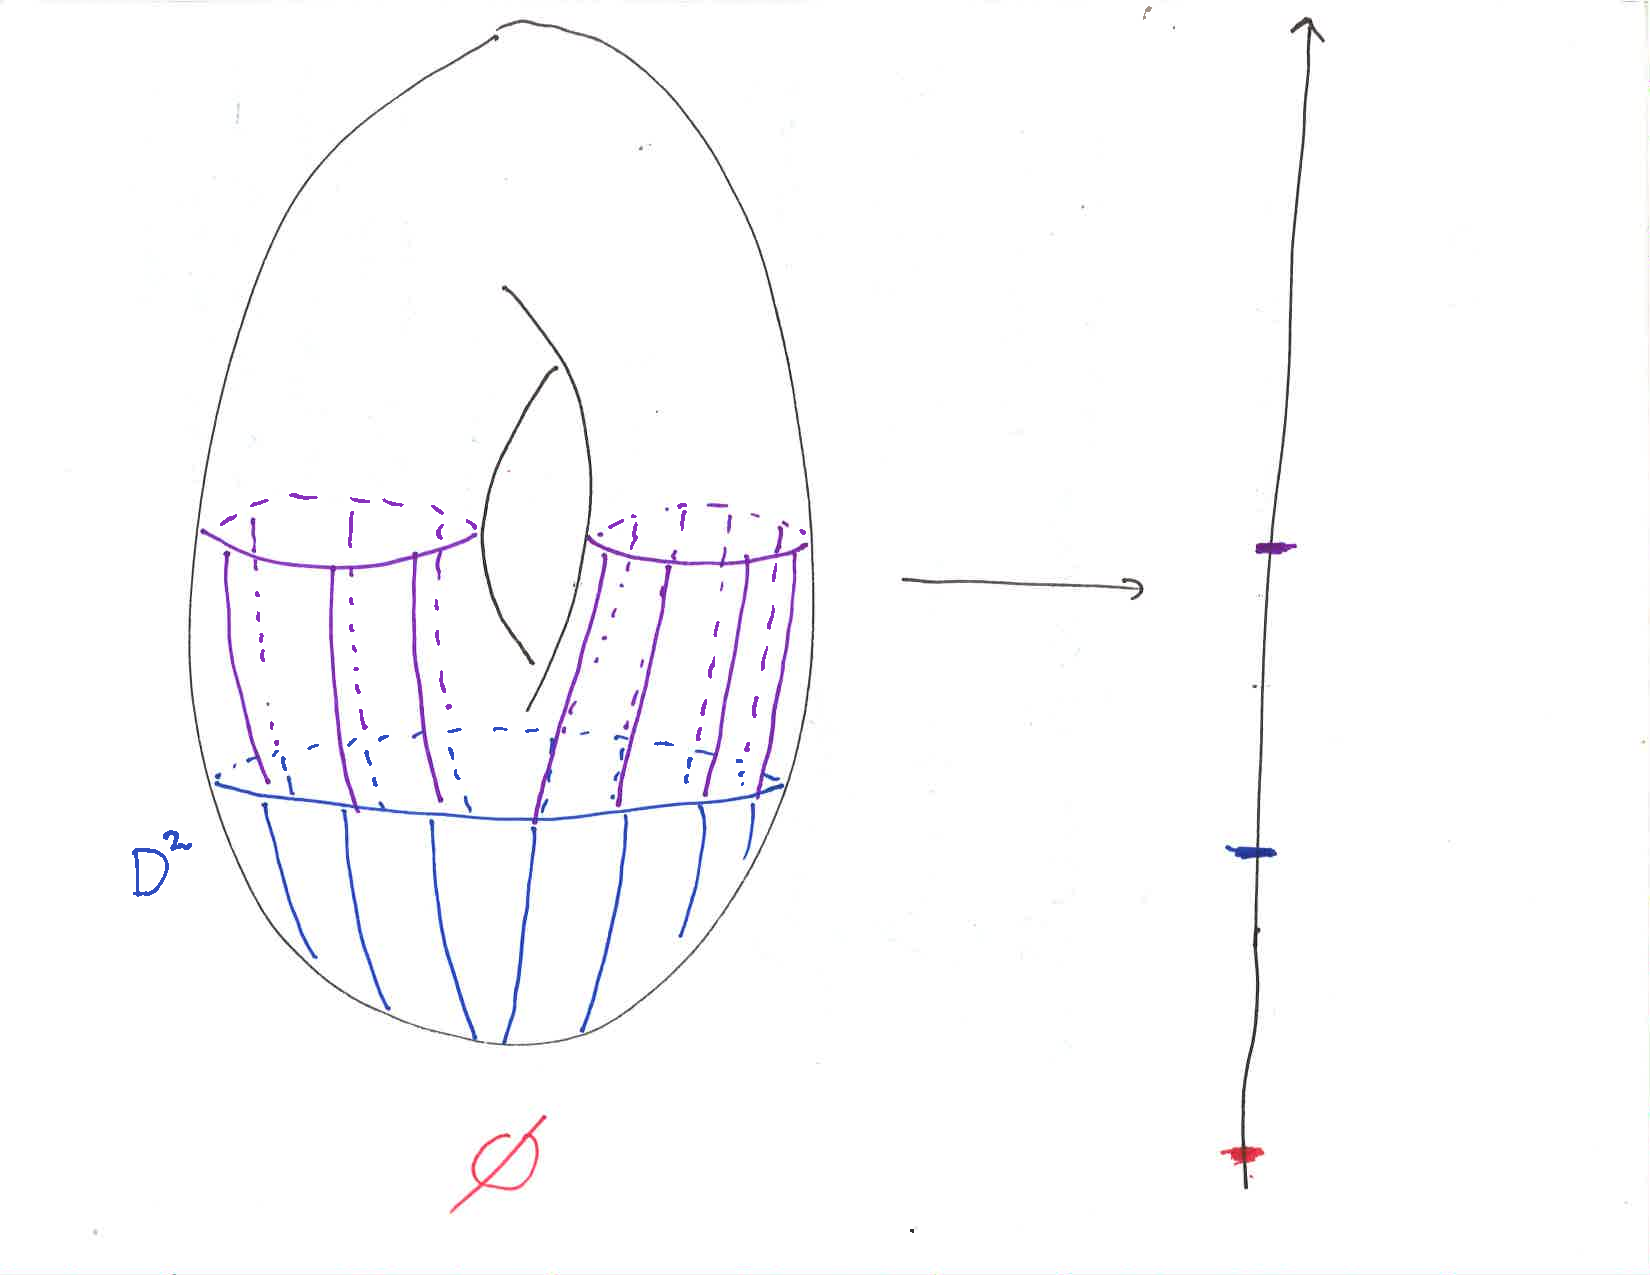
\includegraphics[width=8cm]{torusmorse.pdf}
\caption{A Morse function of the torus given by the height. \label{TorusMorse}}
\end{figure}
A Morse function can be use to obtain a handle decomposition. Let $f: M\to \mathbb{R}$ be a morse function. For each critical point, $p$, fix a coordinate chart centeret at $p$ with coordinates in standard form, i.e., $f(x_1,\ldots,x_m)=f(p)-\sum_{i=1}^k x_i^2+\sum_{j=k+1}^mx_j^2$. 
\begin{definition}
A gradient-like vector field, is a vector field $X$ satisfying the two following conditions:
\begin{enumerate}
\item Near a critical point $p$, $X=\frac{1}{2}\mathrm{grad}(f)$ in the chosen coordinates.
\item For non-critical points $X(f)>0$.
\end{enumerate}
\end{definition}
The factor of $\frac{1}{2}$ comes from the squaring in the standard coordinates. These exists, since we can define them locally, near critical points by the formula above, and away from critical points by choosing a local metric. We can then glue these together by using a partition function.

Suppose $f$ has no critical points on $(a,b)\subset \mathbb{R}$, and fix $b\in (a,b)$, clearly $b$ is a regular value for $f$. Let $Y=f^{-1}(b)$, which is a $(m-1)$ submanifold of $M$, then gicen a gradient-like vector field we get a canonical identification: $Y\times (a,c)\cong f^{-1}((a,c))\subset M$, given by flowing along $X/X(f)$, see figure \ref{nocritpt} for an example.
\begin{figure}[h]
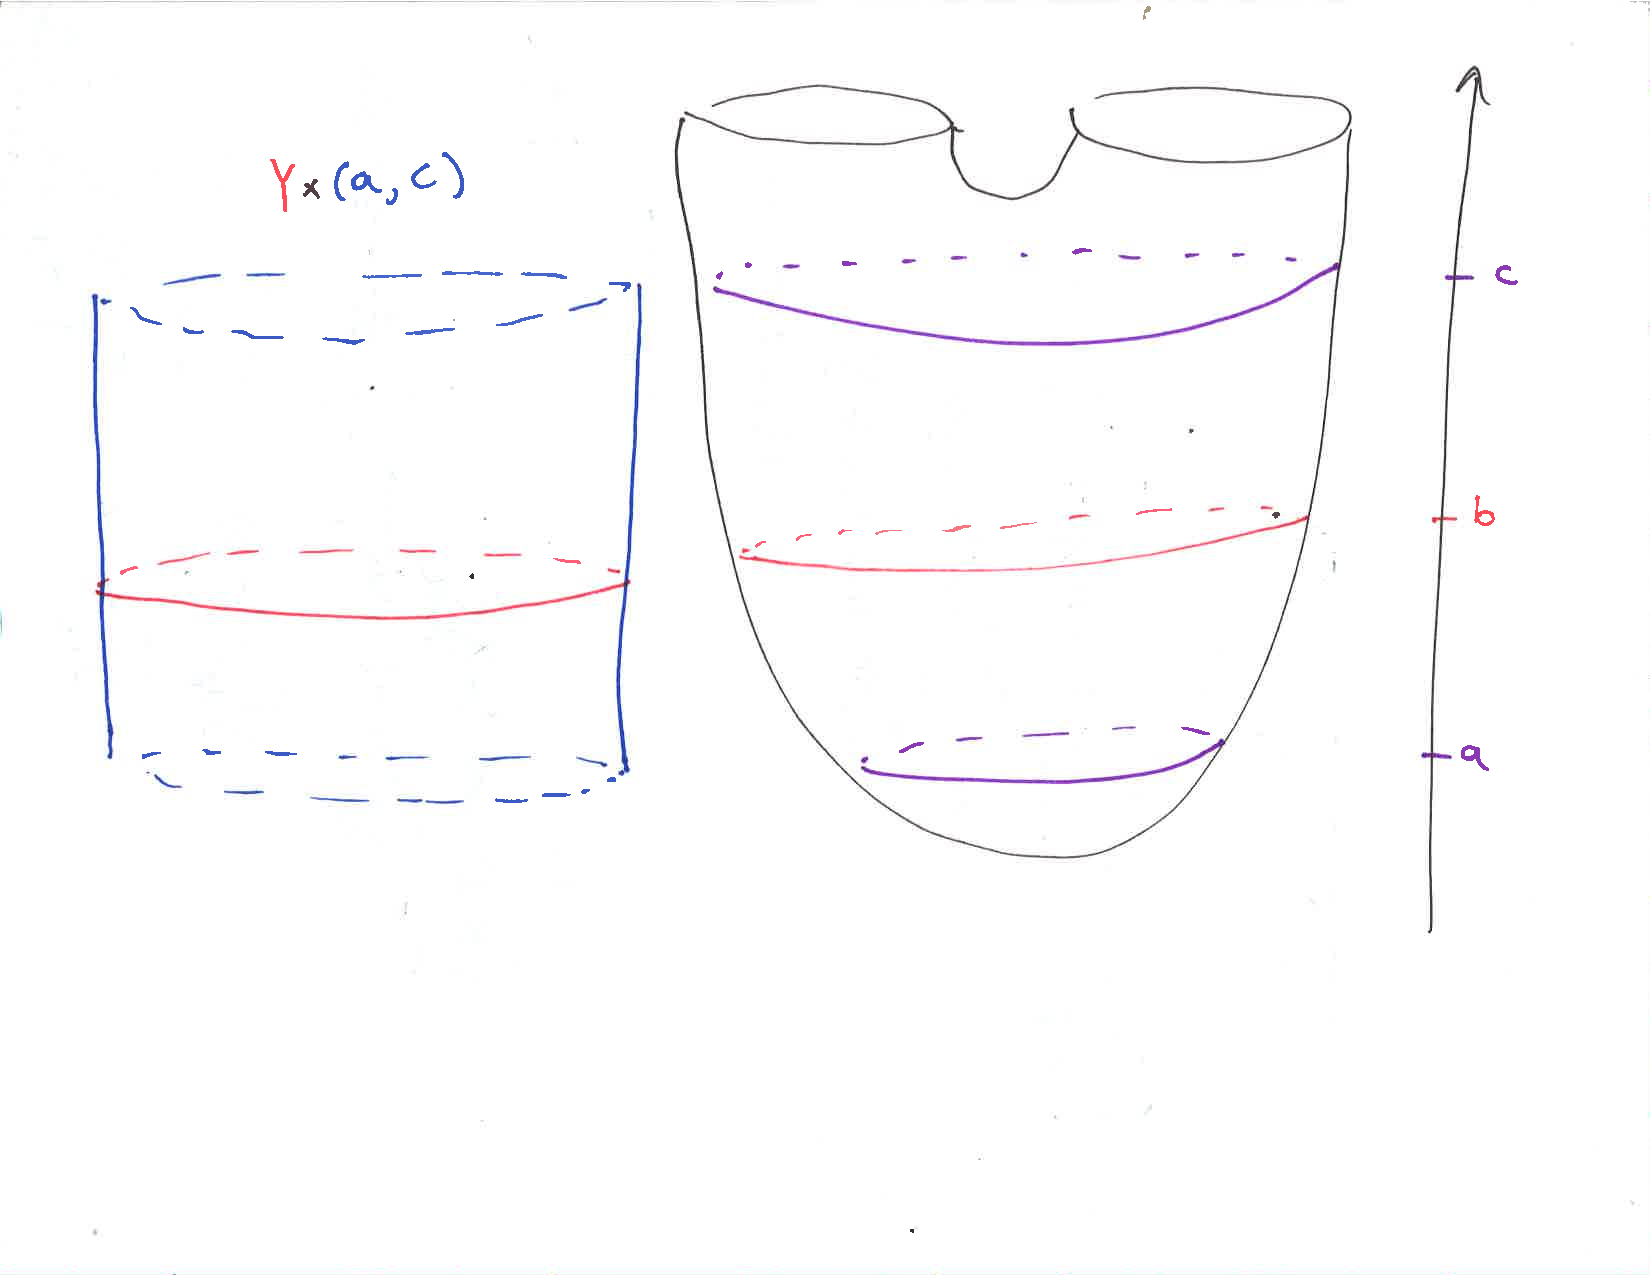
\includegraphics[width=8cm]{nocritpt.pdf}
\caption{Continuing the example from figure \ref{TorusMorse}, we see the identification away from critical points. \label{nocritpt}}
\end{figure}

So now what happens at critical points? Well for most points in the preimage of a critical value of $f$ flowing along $X/X(f)$ is still well defined. So we should think about what happens in a neighbourhood of a critical point. 
Note in figure \ref{TorusMorse} we can obtain the blue part from the redpart by attaching a $0$-handle to the empty set, since the base of a $0$-handle is $\partial D^0\times D^2=\emptyset$, and hence we just get $D^2$. So now the question is how do we move from the blue part to the purple part.
Let $\overrightarrow{x}=(x_1,\ldots, x_k)$, and $\overrightarrow{y}=(x_{k+1},\ldots, x_m)$, and assume for simplicity that $f(p)=0$. Then in coordinates we have that $f(\overrightarrow{x},\overrightarrow{y})=-|\overrightarrow{x}|^2+|\overrightarrow{y}|^2$. We draw the level curves for the value $-1$ in blue, for $+1$ in red, and the curve $|x|\cdot |y|\leq \sinh(1)\cdot \cosh(1) $ in purple in figue . The grey area defined as the interior as these curves form an $m$-disk. By gluing the tales of the level sets together, by flowing along the gradient-like vector field, we can collapse the purple part of the boundary of the disk. We can then identify the thick blue part with $\partial(D^k)\times D^{m-k}$, the base of a $k$-handle, and the thick red part with $D^k\times \partial/D^{m-k})$.
\begin{figure}[h]
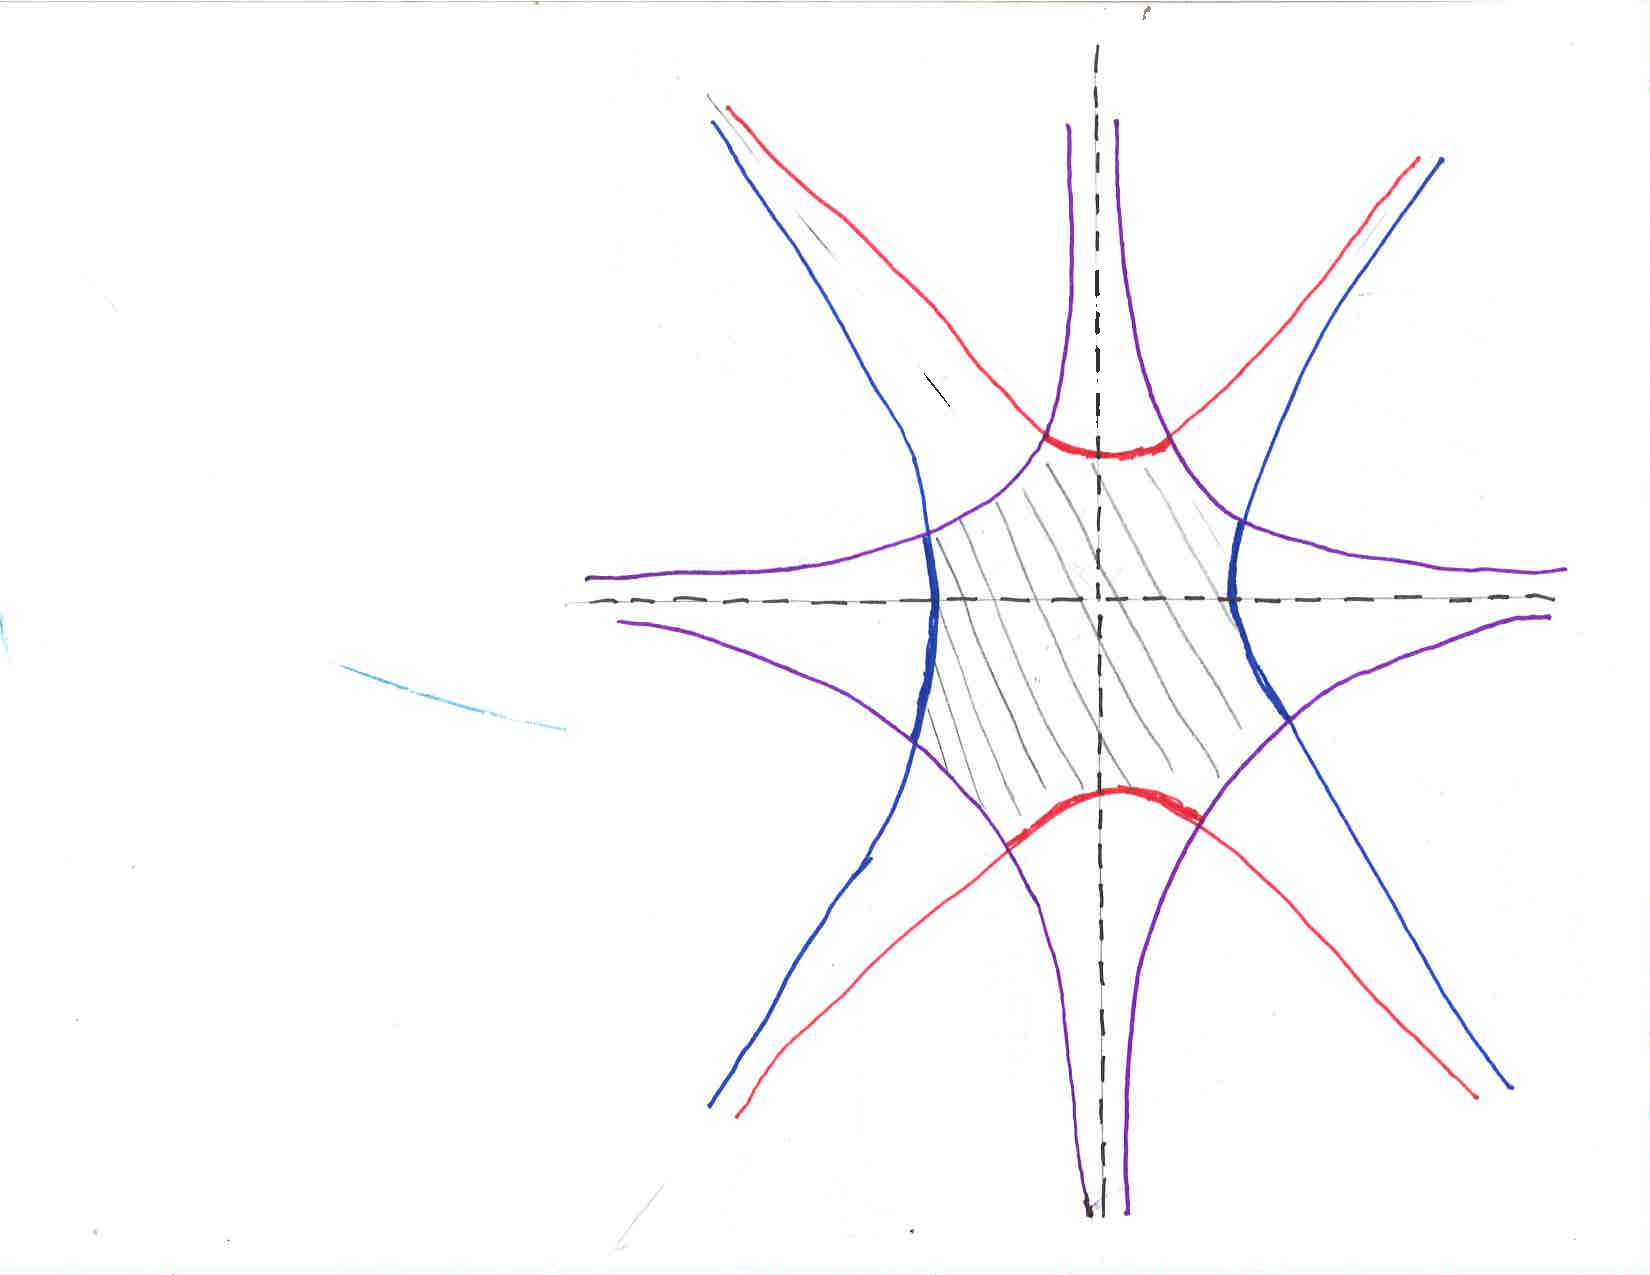
\includegraphics[width=8cm]{lvlset.pdf}
\caption{The levelsets of our morse function at a critical point $p$. \label{lvlset}}
\end{figure}
\begin{figure}[h]
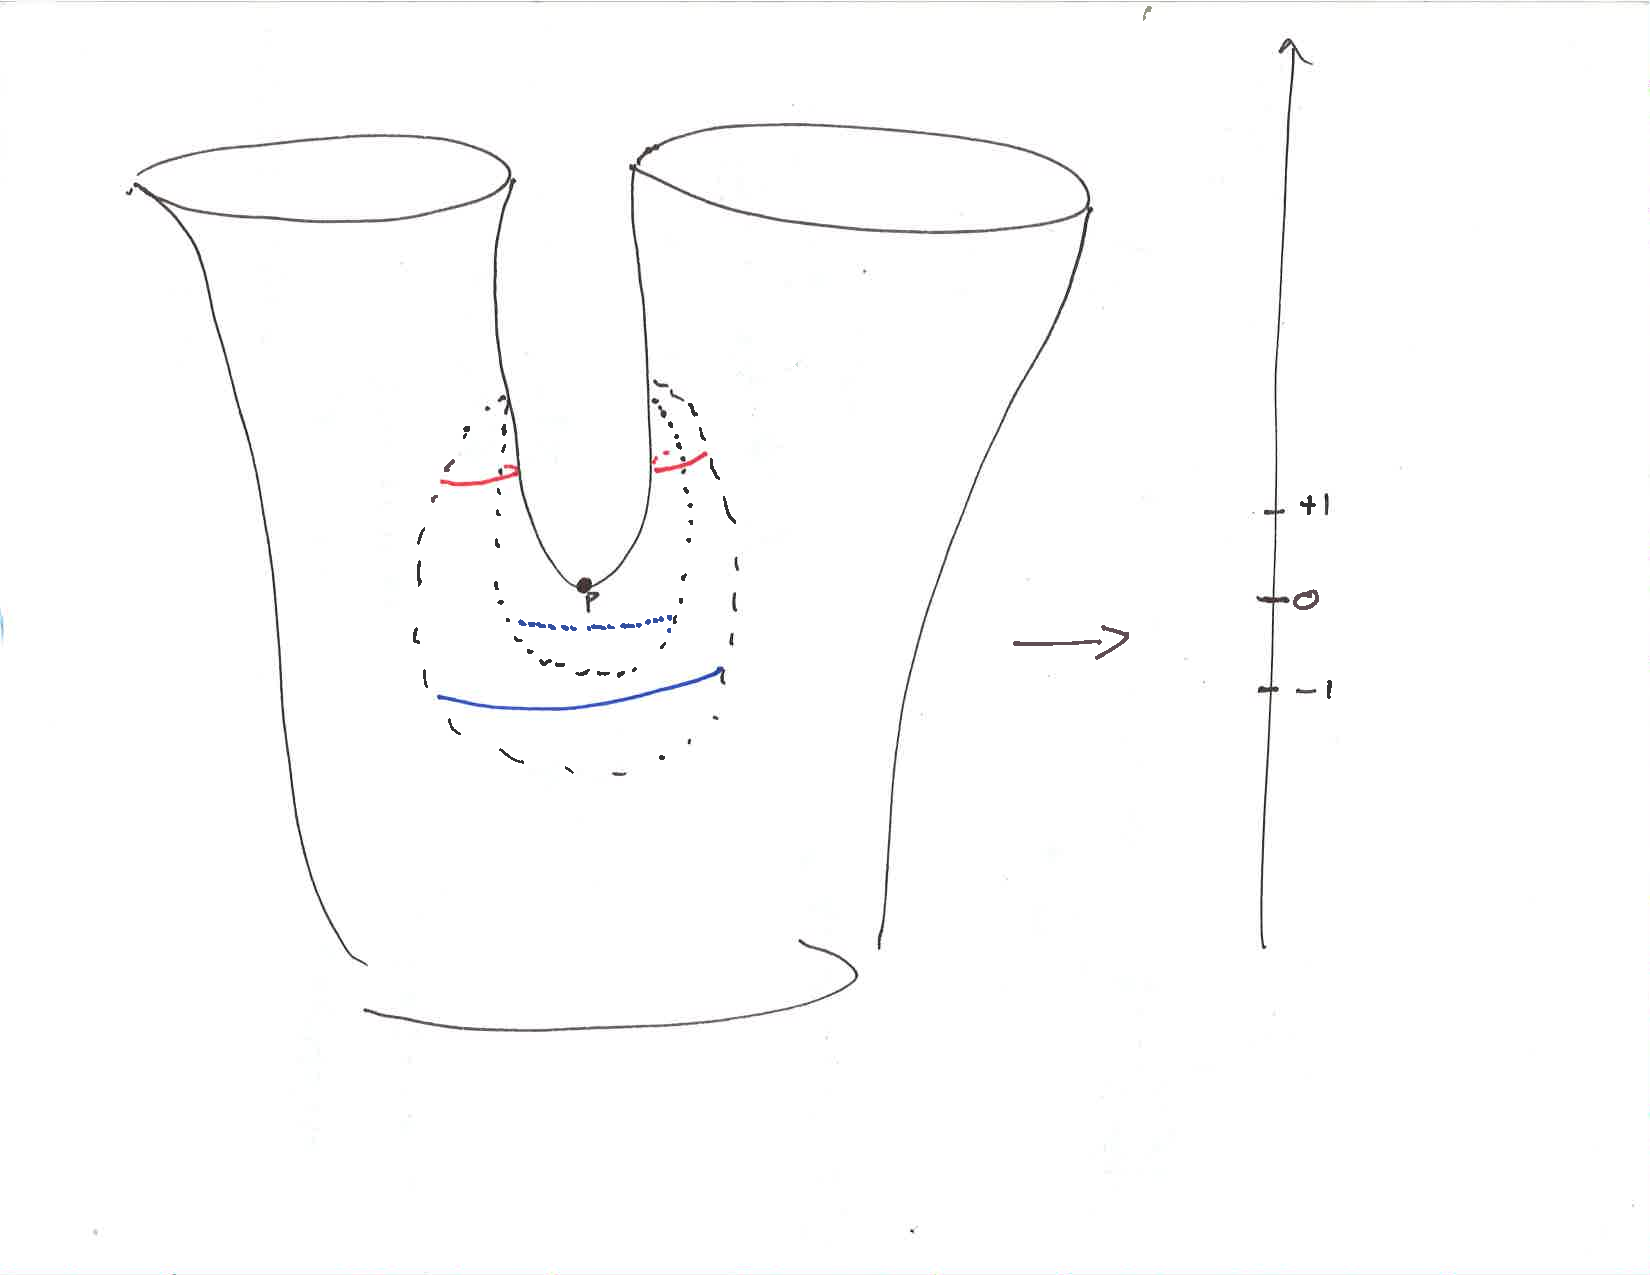
\includegraphics[width=8cm]{critptlvlset.pdf}
\caption{Continuing out example from figure \ref{TorusMorse}, we have the local chart around a critical point $p$, with level sets.}
\end{figure}
We will use the identification of the thick blue part to glue on a
$k$-handle. In our example from figure \ref{TorusMorse} this will look
similar to the gluing in figure \ref{attach1handle}.


%%%%%%%%%%
%
% Insert notes from Feb 28 here
%
%%%%%%%%%%

\section{The h-principle for Open Partial Differential Relations}

% Add some stuff from Feb 28 here

\subsection{Example of $R = J^0(X,Y)$}
\marginnote{\textbf{3/2/2018}}

We will consider first applying our outline for a general proof of the
h-principle to the toy example case of the partial differential
relation $R = J^0(X,Y)$. The space of formal solutions is a functor
$\CF(-) = C^\infty(- , Y)$, while the space of sections of the
$J^0(X,Y)\to X$ defines a functor $\CFh(-) = C^0(-,Y)$. In this case
the h-principle will say that $C^\infty(X,Y) \to C^0(X,Y)$ is a
weak equivalence for any $X,Y$. %% Is it really _any_ that we get?
(Of course, this fact can be seen as a consequence of the classical smooth
approximation theorem.)

We've seen that if $V\subseteq U$ are open and $Y=\R$, then the maps
$C^\infty(U)\to C^\infty(V)$ and $C^0(U)\to C^0(V)$ are not
surjective, that is, the sheaves $C^\infty(-,\R)$ and $C^0(-, \R)$ are
not {\em flabby} and thus cannot be Serre fibrations. On the other
hand, these sheaves are {\em soft}; for any closed subset
$A\subseteq X$, the map $C^\infty(X) \to C^\infty(A)$ is surjective,
when $C^\infty(A)$ is appropriately defined. To find an appropriate
definition, we will work with certain closed submanifolds. Let $\R_+ =
[0,\infty)$. 

\begin{definition} \label{def:neat} Let $X$ be a manifold with
  corners. A subset $X_0\subset X$ is a {\em neat codimension zero
    submanifold} if there is a function $u: X\to \R$ with
  $X_0 = u^{-1}(\R_+)$ such that $u$, its restriction to $\partial X$,
  and its restriction to positive dimensional corner strata are all
  transverse to $0\in \R$.
\end{definition}

So if $X_0\subseteq X$ is neat and $x\in u^{-1}(0)$, then there is a
neighborhood $V\subset X$ of $x$ with local coordinates such that
$X_0 \subseteq X$ looks likes
\[\R_+ \times \R^{m-k-1}\times \R_+^k \subseteq \R\times
  \R^{m-k-1}\times \R_+^k,\] where $m = \dim X$ and $k$ is the
codimension of the corner stratum to which $x$ belongs.

\begin{example}
  The submanifold $A_k = (S^{k-1}\times D^1) \times D^{m-k} \subseteq
  D^k\times D^{m-k}$ is neat.
\end{example}

\begin{definition} \label{def:flexible}
  $\CF$ is {\em flexible} if for every neat $X_0\subseteq X$ the
  restriction map $\CF(X)\to \CF(X_0)$ is a Serre fibration.
\end{definition}

\begin{definition} \label{def:htpyinvt}
  $\CF$ is {\em homotopy invariant} if $\CF(X) \to \CF(X_0)$ is a weak
  homotopy equivalence for all neat $X_0\subseteq X$ such tha the inclusion
  is a homotopy equivalence.
\end{definition}

Our goal for the next two lectures is to show that $C^\infty(-,Y)$ and
$C^0(-, Y)$ are flexible.

\begin{lemma}[Key Lemma (Cor.~\ref{cor:Compact_extension_of_function} below)] \label{lem:compactmapstoRn}
  If $L$ is a compact manifold then $C^\infty(L\times\R, \R^n) \to
  C^\infty(L\times \R_+, \R^n)$ admits a continuous section. 
\end{lemma}

\begin{exercise} \label{ex:vectorspacesection} Prove that any linear
  map $V\to W$ of topological vector spaces that admits a (possibly
  nonlinear) section is a Hurewicz fibration (and hence a Serre
  fibration).
\end{exercise}

\begin{proposition} \label{prop:mapstoRn}
  $C^\infty(-, \R^n)$ is flexible.
\end{proposition}

\begin{proof}
  By \ref{ex:vectorspacesection} it suffices to show that if
  $X_0\subseteq X$ is neat then
  $C^\infty(X,\R^n) \to C^\infty(X_0, \R^n)$ admits a continuous
  section. We will perform a sequence of reductions to be able to
  apply \ref{lem:compactmapstoRn}.

  {\bf Step 1:} We may replace $X$ with any smaller open neighborhood
  $U$ of $X_0$. Indeed, given a section $\overline s: C^\infty(X_0,
  \R^n) \to C^\infty(U, \R^n)$, choose a smooth bump function
  $\rho: X\to [0,1]$ such that $\rho\mid_{X_0} \equiv 1$ and
  $\operatorname{supp}(\rho)\subseteq U$, then define a section
  $s:C^\infty(X_0, \R^n) \to C^\infty(X, \R^n)$ by
  \[
    s(f)(x) = \begin{cases} 0 &x\notin U\\ \rho(x) \overline s(f)(x) & x\in
      U. 
    \end{cases}
  \]

  {\bf Step 2:} We may delete any closed subset $A$ from the interior
  of $X_0$. This is an application of the sheaf gluing property: given
  a family of functions $f_t \in C^\infty(X_0, \R^n)$ with
  restrictions $r(f_t) \in C^\infty(X_0\setminus A, \R^n)$, any family
  of lifts $\widetilde{r(f_t)} : (U\setminus A)\to \R^n$ extends to a
  family of lifts $\tilde f_t : U\to \R^n$.

  {\bf Step 3:} Let $u:X\to \R$ be as in the definition of neat
  manifold, so that $X_0 = u^{-1}(\R_+)$, and let $M = u^{-1}(0)$. By
  replacing $X$ with $U = u^{-1}(-\epsilon,\infty)$ for sufficiently
  small $\epsilon$, by Step 1 we may assume that each component of $X$
  contains exactly one component of $X_0$. By deleting a closed subset
  of the form $u^{-1}([N,\infty))$ for each component of $X_0$, by
  Step 2 we may assume the pair $(X, X_0)$ is isomorphic to $(M\times
  \R, M\times \R_+)$.

  Now choose a locally finite cover $\{U_i\}$ of $M$ such that each
  $\overline U_i$ is compact. Choose a smooth partition of unity
  $\{\phi_i\}$ subordinate to $\{U_i\}$. Then by
  \ref{lem:compactmapstoRn} there are sections 
  \[ s_i : C^\infty(\overline U_i\times \R_+, \R^n) \to C^\infty(\overline
    U_i\times \R, \R^n).\]
  Then the desired map $s: C^\infty(X_0,\R^n) \to C^\infty(X, \R^n)$
  is given by
  \[
    s(f)(x) = \sum_i \phi_i(x) s_i(f)(x).
  \]
\end{proof}

\begin{lemma} \label{lem:c0functorisnice}
  $C^0(-, Y)$ is homotopy invariant and flexible.
\end{lemma}
\begin{proof}
  Take any manifold with corners $X$ with a neat submanifold
  $X_0 \subset X$. Then $(X, X_0)$ is a CW-pair (and in fact an
  NDR-pair).
  %
  % 
  % Find a reference for this? ^^^
  % 
  %
  Flexibility of $C^0(-,Y)$ thus follows immediately by
  \ref{prop:mapsfromcwpair}. To see homotopy invariance of $C^0(-,Y)$,
  define a homotopy equivalence $C^0(X_0, Y) \simeq C^0(X,Y)$ simply
  by precomposing with a homotopy equivalence $X_0 \simeq X$.
\end{proof}

\begin{proposition} \label{prop:mapstonoboundary}
  If $Y$ is a manifold without boundary, then $C^\infty(-, Y)$ is
  flexible. 
\end{proposition}

\begin{proof}
  Fix a manifold with boundary $X$ and neat submanifold
  $X_0\subseteq X$. Fix a smooth embedding $Y\to \R^n$ for
  sufficiently large $n$, and find $N\subseteq \R^n$ a tubular
  neighborhood of $Y$. There is a smooth retraction $r: N \to Y$
  by regarding $N$ as the normal bundle and using scalar
  multiplication. Postcomposition with $r$ shows that
  $C^\infty(X,Y)\to C^\infty(X_0, Y)$ is a retract of
  $C^\infty(X, N) \to C^\infty(X_0, N)$. Therefore by \ref{RLPclosed}
  it suffices to show that $C^\infty(X, N) \to C^\infty(X_0, N)$ is a
  Serre fibration.

  We need to solve the lifting problem
  \begin{equation*}
    \begin{tikzcd}
      D^\ell \times \{0\} \arrow[r] \arrow[hookrightarrow]{d}
      & C^\infty(X,N) \arrow[d] 
      \\
      D^\ell \times I \arrow[r] \arrow[dashed,ur] 
      & C^\infty(X_0, N) 
    \end{tikzcd}
  \end{equation*}
  Postcomposition with the inclusion $N\to \R^n$ extends this to a
  diagram
  \begin{equation*}
    \begin{tikzcd}
      D^\ell \times \{0\} \arrow[r] \arrow[hookrightarrow]{d}
      & C^\infty(X,N) \arrow[d] \arrow[r]
      & C^\infty(X, \R^n) \arrow[d] 
      \\
      D^\ell \times I \arrow[r] \arrow[dashed, urr]
      & C^\infty(X_0, N) \arrow[r]
      & C^\infty(X_0, \R^n)
    \end{tikzcd}
  \end{equation*}
  This lifting problem has a solution
  $h: D^\ell\times I \to C^\infty(X,\R^n)$ by \ref{prop:mapstoRn}. We
  want to modify $h$ so that $h(a,t)(x)\in N$ for all $a\in D^\ell$,
  $t\in I$, and $x\in X$.

  We know already that $h(a,t)(x_0) \in N$ for all $x_0\in X_0$, and
  that $h(a,0)(x)\in N$ for all $x\in X$. Therefore there is a
  %
  %
  smooth %%% continuous? %%%
  % 
  % 
  ``first escape'' function $\epsilon :X\to (0,1]$ such
  that $h(a,t)(x)\in N$ for all $a\in D^\ell$ and
  $0 < t \leq \epsilon(x)$, and such that
  $\epsilon \mid_{X_0} \equiv 1$. Let 
  \[
    X\times [0,\epsilon] = \{ (x,t) \mid 0\leq t \leq \epsilon(x) \}
  \]
  There is a diffeomorphism
  $\phi: X\times [0,1] \cong X\times [0,\epsilon]$. Let $\tilde h$ be
  the composition of $\phi$ with the restriction of $h$ to $X\times
  D^\ell \times [0,\epsilon]$. This solves the desired lifting problem.
\end{proof}

Out next goal is to prove that $C^\infty(-,Y)$ is homotopy invariant. Suppose that $X_0\subseteq X$ is neat and the inclusion is a homotopy equivalence. Neatness implies that $X$ deformation retracts onto $X_0$ continuously. However, for our purposes, we need smooth maps, and there there may exist no smooth deformation retraction.
\begin{example}
  Let $X_0 = (-\infty,0]$ and $X=\R$. Then $X_0\subset X$ is neat and a homotopy equivalence, so let $H:X\times I\to X$ be a deformation retraction, that is:
  \begin{itemize}
  \item $H_0(x)=x$ for all $x\in X$,
  \item $H_1(x)\in X_0$ for all $x\in X$, and
  \item $H_t(x_0)=x_0$ for all $t\in I$ and $x\in X_0$.
  \end{itemize}
 Then, $H_1$ cannot be differentiable at 0. We have
\[
\lim_{h\to0^-}\frac{H_1(h)}{h} = 1
\]
since $H_1$ is the identity on $(-\infty,0]$. But
\[
\lim_{h\to0^+}\frac{H_1(h)}{h} \le 0
\]
since $H_1(h)$ must be nonpositive for $h>0$, while $h$ itself is positive. Thus $H_1$ is not smooth.
\end{example}
\begin{lemma}
  If $X_0\subset X$ is neat and a homotopy equivalence, then there is exists a map $H:X\times I\to X$ such that
  \begin{itemize}
  \item $H_t: X\to X$ is smooth for each $t$,
  \item $H_0 = \id_X$,
  \item $H_1(x)\in X_0$ for all $x\in X$, and
  \item $H_t(y)\in X_0$ for all $t\in I$, $y\in X_0$.
  \end{itemize}
Note the weakening in the last condition: the map isn't required to be the identity on $X_0$, but just to map $X_0$ to itself.
\end{lemma}
\begin{proof}
  We will prove this by starting with a continuous deformation retract and massaging it, then applying a smooth approximation theorem.

\noindent  \textbf{Step 1:} Make a tubular neighborhood of $u^{-1}(0)$.

  Let $u:X\to \R$ be such that $X_0=u^{-1}(\R_+)$, and set $A=u^{-1}(0)$. $A$ is a codimension 1 submanifold, and moreover, nearby to a point of $A$, $X_0$ looks like the inclusion
  \[  
    \R_+\times \R^{m-k-1}\times \R_+^k\subset \R\times \R^{m-k-1}\times \R^k_+.
  \]
  $A$ is the subset of the left-hand side with first coordinate 0. So, there exists a tubular neighborhood, which here is a smooth embedding
  \[
    A\times \R\to X.
  \]
  Let $N=A\times \R$ as a subset of $X$.\\

\noindent  \textbf{Step 2:} Build a smooth map $X\times I\to X$ which is constant outside $N$, and near the origin inside of $N$ sends $A\times\{0\}$ to $A\times\{-1\}$.

  Using bump functions on $\R$, we find find a continuous family of smooth maps $\phi_t:\R \to \R$ for $t\in I$ such that $\phi_t(0)=-t$, $\phi_t$ is the identity outside of a neighborhood of $0$, and $\phi_t$ is monotonic (thus a diffeomorphism). We can extend $\phi_t$ to be a function $X\to X$ by setting $\phi_(a,r)=(a,\phi_t(r))$ on $N$, and $\phi_t$ is the identity outside of $N$, as in Figure~\ref{fig:phi_t}.

  \begin{figure}[h]
    
  \centering
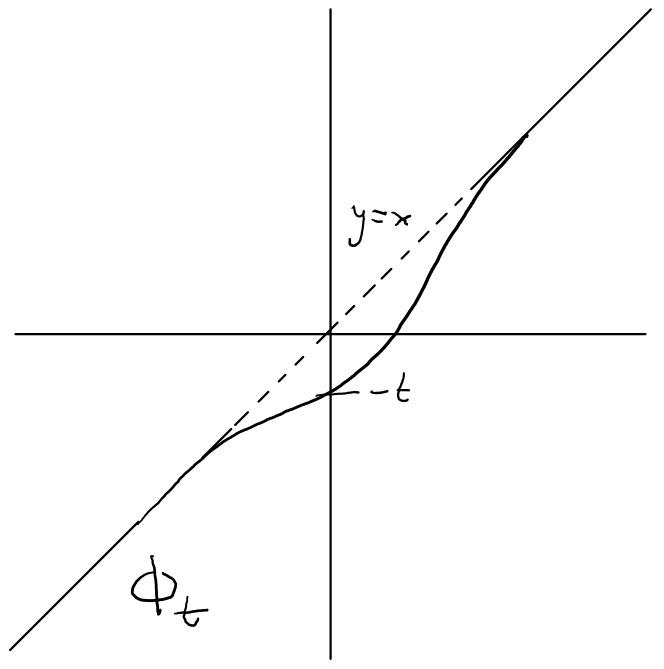
\includegraphics[width=5cm]{phi_t_2}
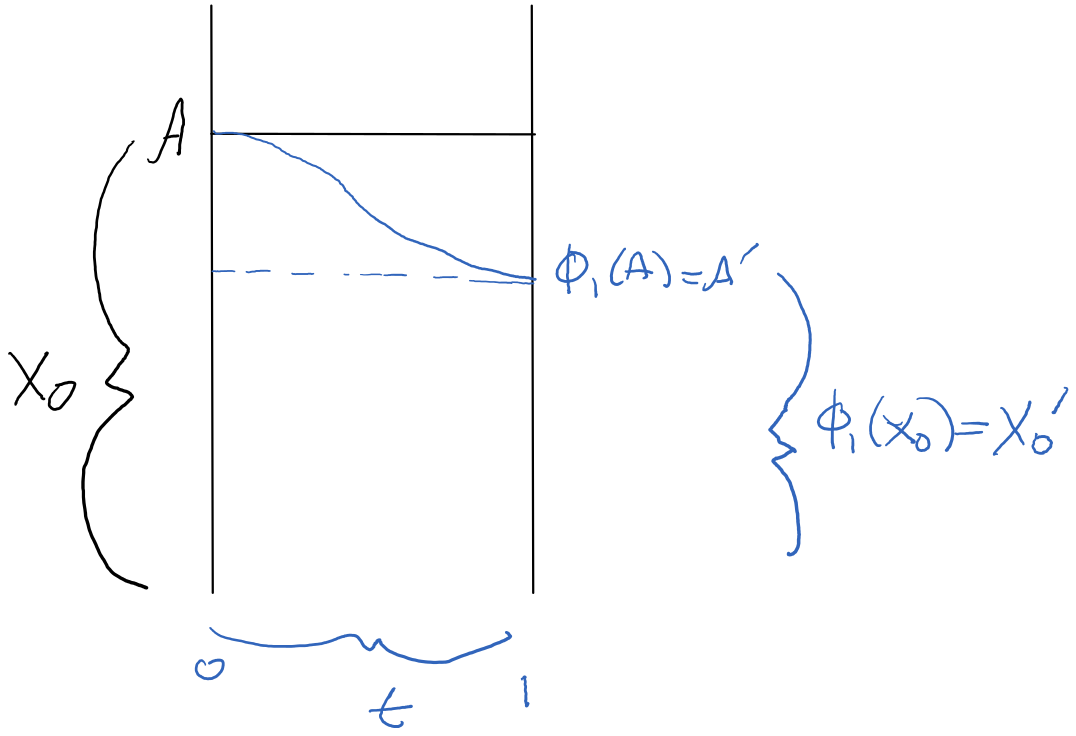
\includegraphics[width=7cm]{phi_t}
\caption{Left: $\phi_t$ as a function $\R\to\R$. Right: $\phi$ shifts down $X$, pushing a neighborhood of $A$ into $X_0$.\label{fig:phi_t}}
\end{figure}


\noindent  \textbf{Step 3:} Combine the continuous deformation retract with the smooth translation function to set up for smooth approximation.

  Let $H':X\times I\to X$ be a continuous deformation retraction to $X_0$. Let $H'': X\times I\to X$ be given by
  \[
    H''_t = \phi_t\circ H'_t\circ \phi_t.
  \]

  \begin{figure}[h]
    \centering
    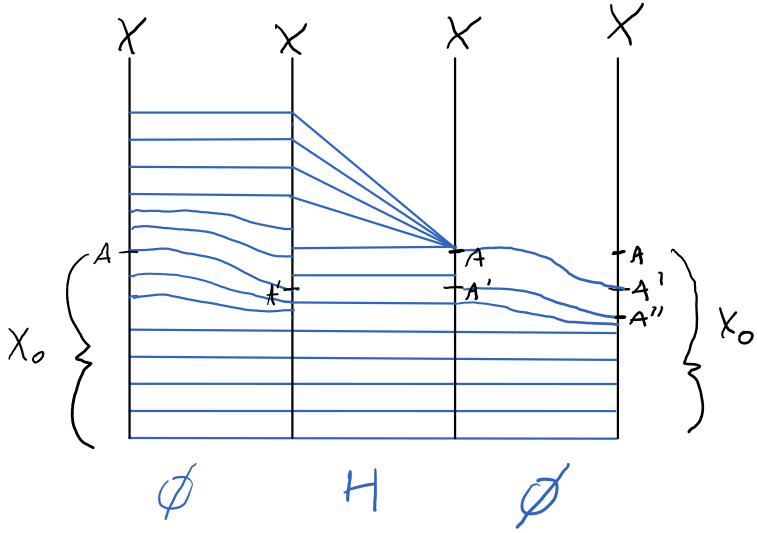
\includegraphics[width=8cm]{smooth_retraction}
    \caption{A continous homotopy on $X$ whose image is in the interior of $X_0$.\label{fig:smooth_retraction}}
  \end{figure}
  This map, shown in Figure~\ref{fig:smooth_retraction}, is smooth on a neighborhood of $X_0$ by the construction of $\phi$, and the $H''_t(X_0)\subseteq X_0$ for all $t$. Furthermore, we can take $H'$ to be constant for small $t$ such that $H''$ is smooth on a neighborhood of $X_0\times I\cup X\times\{0\}$.\\

\noindent\textbf{Step 4:} Use relative smooth approximation.

  We now apply the following theorem to $H''$:
  \begin{theorem}
    Let $f:M\to Y$ be a continuous map of smooth manifold, and let $Z\subseteq M$ be a closed subset. Suppose that $f$ is smooth on a neighborhood of $Z$. 
    Then, for any open neighborhood of $f$ in the strong $C^0$ topology on $C^0(M,Y)$, there is a smooth $g:M\to Y$ such that $g$ and $f$ agree on an open neighborhood of $Z$.
  \end{theorem}

  By step 3, there exists a function $\epsilon: X\to \R_{\ge 0}$ such that for all $x,$
  \[
B_{\epsilon(x)}(H''_1(x))\subseteq \Int(X_0)
\]
(I'm not sure what exactly the left hand side means, I think we can interpret it with the neatness function $u$?) So we apply the theorem with
\[
  M = \{H:X\times I\to X\mid d(H(x,t), H''(x,t))<\epsilon(x)\text{for all }x\in X, t\in I\}
\]
to obtain our desired $H$.
\end{proof}
\begin{proposition}
  $C^\infty(-,Y)$ is homotopy invariant.
\end{proposition}
\begin{proof}
  Let $X_0\subseteq X$ be neat and a homotopy equivalence.
Let $H:X\times I\to X$ be a homotopy as in the lemma.
We will show $C^\infty(X,Y)\to C^\infty(X_0,Y)$ is a weak equivalence by solving the lifting problem
\[
  \begin{tikzcd}
    \partial D^k\arrow[r]\arrow[d] & C^\infty(X,Y)\arrow[d]\\
    D^k\arrow[r]\arrow[ur,dashed] & C^\infty(X_0,Y)
  \end{tikzcd}
\]
up to homotopy rel boundary in the bottom triangle. In order to construct such a lift, we will write
\[
  D^k = \partial D^k\times \left[0,\tfrac12\right]\bigcup_{\partial D^k\times\left\{\tfrac12\right\}}D^k_{\tfrac12}
\]

\begin{figure}[h]
  \centering
  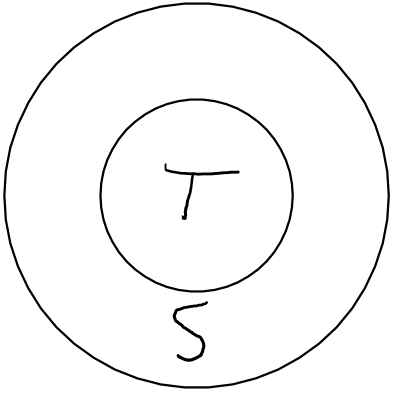
\includegraphics[width=4cm]{disk_s_t}
    \caption{The disk as a union of a cylinder and a smaller disk.\label{fig:disk_s_t}}
\end{figure}
Write 
\[
S = \partial D^k\times \left[0,\frac12\right]
\]
and
\[
T = D^k_{\tfrac12} 
\]
as shown in Figure~\ref{fig:disk_s_t}.
Our outer square gives us maps $f: D^k\times X_0\to Y$ and $f_0: \partial D^k\times X\to Y$ which are smooth in the second coordinate. Since we have already proven flexibility, we can lift $f|_S$ to some
\[
  g: S\times X \to Y
\]
such that $g|_{t=0}=f_0$. Define
\[
  \tilde f: D^k\times X\to Y
\]
as 
\[
  \tilde f(d, x) =
  \begin{cases}
    g(d, H(x,2t)) & d\in S\\
    f(d, H(x,1)) & d\in T
  \end{cases}
\]
where $t$ is the interval coordinate on $S$.
This map for $t=0$ is exactly equal to to $f_0$ since $H_0 = \id_X$. The bottom triangle doesn't commute on the nose, but it does up to homotopy. Define a homotopy $G: I\times D^k\times X_0 \to Y$ as
\[
G_s(d,x_0) =   \begin{cases}
    g(d, H(x,2ts)) & d\in S\\
    f(d, H(x,s)) & d\in T
  \end{cases}.
\]
Then, for $s=1$, we recover $\tilde f|_{X_0}$, and for $s=0$, we recover the original $f$.
\begin{figure}[h]
  \centering
  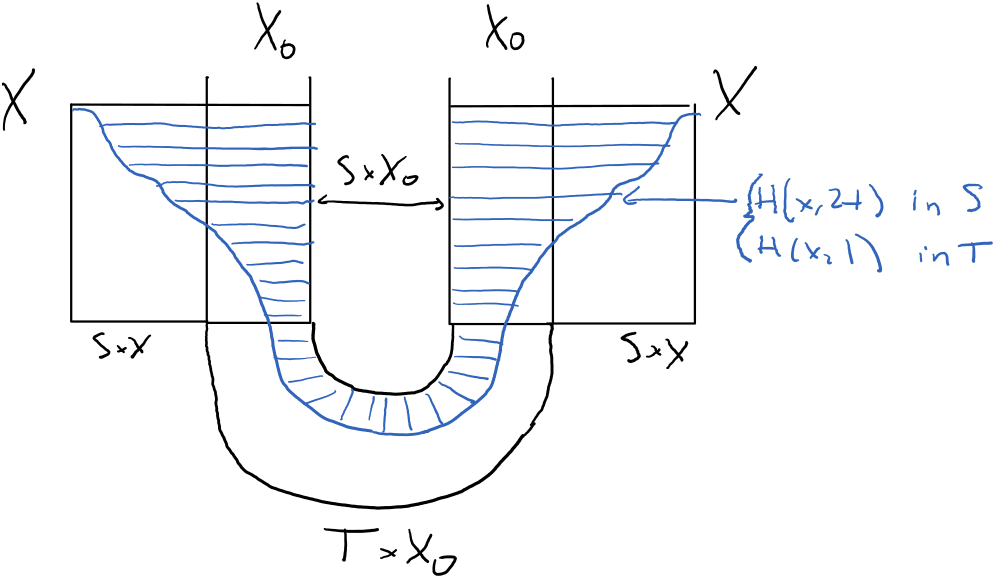
\includegraphics[width=10cm]{htpy_invariant}
  \caption{$\tilde f$ for $k=1$.}
\end{figure}
\end{proof}


\subsection{A surprising lemma of \'Emile Borel}

In this section we will prove a somewhat technical lemma which is the key to proving that the sheaf $C^\infty(-,Y)$ is a flexible sheaf. The material of this section is mostly taken from Michael Weiss' excellent notes on immersion theory. 



Let $V$ be a finite dimensional vector space and consider the space $C^\infty(\R, V)$ of smooth $V$-valued functions on the line. Taking derivatives at the origin gives us a map,
\begin{equation*}
	j^r_0: C^\infty(\R, V) \to J^r_0(\R, V) \cong \prod_{i=0}^r V,
\end{equation*}
and we have seen that there is a smooth section. Specifically a smooth section is provided by the polynomial equation:
\begin{equation*}
	(v_i)_{i=0}^{r} \mapsto \sum_{k=0}^r \frac{x^k}{k!} \cdot v_k.
\end{equation*}

In this section we will extend this idea in two directions. First we will let $r \to \infty$ and second we will replace $V$ with  (something similar to) the infinite dimensional vector space $C^\infty(L, \R)$ for some $n$-manifold $L$. 

Although it seems easier, already the first generalization, letting $r \to \infty$, has most of the technical difficulties. We cannot simply use the above polynomial expression since in general this will (drastically) fail to converge to a smooth function. Specifically the behavior of the $r^\textrm{th}$-order polynomial expressions will vary erratically near the ends of $\R$. 

We can try to fix this by utilizing a bump function. 
Choose, once and for all, a smooth function $\rho: \R \to [0, \infty)$ such that $\rho \equiv 1$ in a neighborhood of $0 \in \R$, and such that $\rho$ vanishes outside the interval $[-1,+1]$. In general the naive guess $\sum \frac{x^i}{i!} \rho(x) v_i$ will still fail to converge. Instead we may look for an expression of the form:
\begin{equation*}
	(v_i)_{i=0}^\infty \mapsto \sum_{k=0}^\infty \frac{x^k}{k!} \rho(\mu_k x) \cdot v_k.
\end{equation*}
where the $\mu_k \geq 1$ are scalar factors which depend continuously on the $v_i$'s. 


\begin{lemma}
	There exists a continuous section of the infinite order jet prolongation map:
	\begin{equation*}
		j^\infty_0: C^\infty(\R, V) \to J_0^\infty(\R, V) \cong \prod_{i=0}^\infty V
	\end{equation*}
	(where, as usual, the right-hand-side is given the product topology).
\end{lemma}

\begin{proof}
	As proposed above, the section will be given by an expression of the form
	\begin{equation} \label{eqn:Section_formula_1}
		(v_i)_{i=0}^\infty \mapsto \sum_{k=0}^\infty \frac{x^k}{k!} \rho(\mu_k x) \cdot v_k = f(x).
	\end{equation}
	where the $\mu_k$ depend continuously on the $v_i$'s. 
	%Let $f_r(x)$ be defined by the partial sum
	%\begin{equation*}
	%	f_r(x) =  \sum_{k=0}^r \frac{x^k}{k!} \rho(\mu_k x) \cdot v_k.
	%\end{equation*}
	We must find continuous expressions for the $\mu_i$'s which ensure that each for each $r$, the series of functions
	\begin{equation} \label{eqn:Partial_derivative_sequence}
		\sum_{k=0}^\infty \frac{\partial^r}{\partial x^r} \left( \frac{x^k}{k!} \rho(\mu_k x) \cdot v_k \right)
	\end{equation}
	converges uniformly on $\R$. 
	
	Let $\psi_i(x) := (i!)^{-1} x^i \rho(x)$. Then the $i^\textrm{th}$-term of Equation (\ref{eqn:Section_formula_1}) is given by $(\mu_i)^{-i} \psi_i(\mu_ix) v_i$. Let $M_i$ be defined by
	\begin{equation*}
		M_i := \max_{\substack{r < i \\ x \in [-1,1]}} \left\{ \frac{\partial^r}{\partial x^r} \psi(x) v_i \right\}.
	\end{equation*}
	This is a continuous function of $v_i$. 
	
	By construction (and using the assumption that each $\mu_i \geq 1$, and that $\rho$ is identically zero outside $[-1,+1]$) we obtain that when $i \geq r$, the $i^\textrm{th}$-term of the series (\ref{eqn:Partial_derivative_sequence}) is bounded (at each point of $\R$) by 
	\begin{equation*}
		|i^\textrm{th}\textrm{-term of (\ref{eqn:Partial_derivative_sequence})}| \leq (\mu_i)^{-i} (\mu_i)^r M_i \leq M_i \mu_i^{-1}. 
	\end{equation*}
	Thus setting $\mu_i = \max \{1, 2^i M_i \}$ (which again is continuous in $v_i$) ensures that for each $r$ the series (\ref{eqn:Partial_derivative_sequence}) is uniformly bounded. Hence equation (\ref{eqn:Section_formula_1}) defines a smooth $V$-valued function $f(x)$ on $\R$. This gives us a set-theoretical section of $j^\infty_0$. 
	
We will now show that the assignment
\begin{equation*}
	s: \nu = (v_i)_{i=0}^\infty \mapsto f_\nu(x) = \sum_{k=0}^\infty \frac{x^k}{k!} \rho(\mu_k x) \cdot v_k
\end{equation*}
  is continuous in $\nu \in \prod_{i=0}^\infty V $. Let $U \subseteq C^\infty(\R, V)$ be an open subset and let $\nu_0 \in s^{-1}(U)$. It will suffice to show that there exists an open neighborhood of $\nu_0$ contained in $s^{-1}(U)$. Set $f_0 = s(\nu_0)$.

Recall that we have a neighborhood basis of open subsets of $C^\infty(\R, V)$ for the weak $C^\infty$-topology given by
\begin{equation*}
	B^{(r)}_{\delta,K}(f_0) = \{ f \in C^\infty(\R, V) \; | \; \sup_{x \in K}|| j^rf(x) - j^rf_0(x) || < \delta \}
\end{equation*} 
where $r$ is a non-negative integer, $K \subseteq \R$ is compact, $\delta > 0$, and $f_0 \in C^\infty(\R, V)$. Thus there exists such a $B^{(r)}_{\delta, K}(f_0)$ contained in $U$. 

For each fixed $p$ and each $r$ we may write the series (\ref{eqn:Partial_derivative_sequence}) as a sum of two terms:
\begin{equation*}
		\underbrace{\sum_{k=0}^p \frac{\partial^r}{\partial x^r} \left( \frac{x^k}{k!} \rho(\mu_k x) \cdot v_k \right)}_{S_{p,r}(\nu)}
		+ 	\underbrace{\sum_{k=p+1}^\infty \frac{\partial^r}{\partial x^r} \left( \frac{x^k}{k!} \rho(\mu_k x) \cdot v_k \right)}_{R_{p,r}(\nu)}.
\end{equation*}
Because $\mu_i$ depends continuously on the single coordinate $v_i$, the first of these two terms, $S_{p,r}(\nu)$, is a continuous function in $\nu$. It follows that each $S_{p,0}^{-1}(B^r_{\epsilon, K}(f_0))$ is an open subset of $ \prod_{i=0}^\infty V $. 

Moreover whenever $p>r$, the second term, $R_{p,r}(\nu)$, is bounded by
\begin{equation*}
	\frac{1}{2^{p+1}}+ \frac{1}{2^{p+2}}+ \frac{1}{2^{p+3}}+ \cdots = \frac{1}{2^p}.
\end{equation*} 
By choosing $p$ large enough, we can make this term as small as we wish. Thus it follows that there exists an open neighborhood of $\nu_0$ lying entirely within $s^{-1}(B^{(r)}_{\delta, K}(f_0))$. Hence $s$ is continuous.
\end{proof}

The next lemma is conceptually very similar with $V$ replaced by the infinite dimensional vector space $C^\infty(L)$ of smooth functions on a compact manifold $L$. However in this case we interpret `$C^\infty(\R, C^\infty(L))$' as $C^\infty(\R \times L)$. Thus in some sense we are treating $C^\infty(L)$ as a generalized smooth (vector) space. It is possible to formulate the next lemma in that generality, but we will not attempt to do so.  

\begin{lemma} \label{lma:Extend_Derivatives_to_function}
	Let $L$ be a compact manifold. The map $C^\infty(\R \times L, \R^n) \to \prod_{k=0}^\infty C^\infty(L, \R^n)$ given by
	\begin{equation*}
		f(x,y) \mapsto \left( \frac{\partial^k f}{\partial x^k}  |_{\{0\}\times L} \right)_{k=0}^\infty
	\end{equation*}
	has a continuous section. 
\end{lemma}

\begin{proof}
	The proof is nearly identical to the previous one, with the following minor changes:
	\begin{itemize}
		\item The vectors $v_i$ are now smooth functions $f_i(y)$ on $L$. 
		\item The partial derivatives $\frac{\partial^r}{\partial x^r}$ in the series (\ref{eqn:Partial_derivative_sequence}) must be replaced with multivariable partial derivatives $D^\alpha$ for every multi-index $\alpha$. In general each instance of an `$r$' will be replaced with a multi-index `$\alpha$'.
		\item For example the number $M_i$ is the maximum value of functions involving partial derivatives $D^\alpha$ where $|\alpha| < i$. The maximum is taken over $[-1.+1] \times L$ (which is still compact).  
	\end{itemize}
	Otherwise the proof is essentially identical to the previous one. 
\end{proof}

\begin{corollary} \label{cor:Compact_extension_of_function}
	Let $L$ be a compact manifold, as above. Then the restriction map 
	\begin{equation*}
		C^\infty(L \times \R, \R^n) \to C^\infty(L \times [0,\infty), \R^n)
	\end{equation*}
	admits a continuous section. In particular it is a Serre fibration. 
\end{corollary}

\begin{proof}
	The last statement follows because any linear map of topological vector spaces which admits a (not necessarily linear) continuous section is a Serre fibration, in fact a Hurewicz fibration. We leave this part as an exercise.  
	
	For the rest, consider a given $f \in C^\infty(L \times [0,\infty), \R^n)$. Let $x$ denote the coordinate in the $\R$-direction of $L \times \R$. We have the sequence
	\begin{equation*}
		\left( \frac{\partial^k f}{\partial x^k}|_{L \times \{0}  \right)_{k=0}^\infty
	\end{equation*}
	which depends continuously on $f$. Applying Lemma \ref{lma:Extend_Derivatives_to_function}, there exists a smooth function $\tilde{f}: L \times \R \to \R^n$, whose $x$-derivatives agree with those of $f$ along $L \times {0}$. The construction of $\tilde{f}$ is continuous in the above sequence of partial derivatives, hence continuous in the original $f$. Moreover for each multi-partial derivative we have $D^\alpha \tilde{f}|_{L \times \{0\}} = D^\alpha f|_{L \times \{0\}}$. Thus we may define $g:L \times \R \to \R^n$ by
	\begin{equation*}
		g(w,x) = \begin{cases}
			\tilde{f} (w,x) & x \leq 0 \\
			f(w,x) & x \geq 0
		\end{cases}
	\end{equation*}
Since the derivatives of $f$ and $\tilde{f}$ agree along $L \times \{0\}$, all the derivatives of $g$ exist and are continuous. Hence $g$ is a smooth function.
\end{proof}

\subsection{The H-principle for flexible sheaves}

We are ready to prove a metatheorem from which many instances of the H-principle will flow.

\begin{theorem}\label{thm:flexible-h-princ}
Let $\mathcal{F}$ and $\mathcal{F}^h$ be sheaves of spaces on $m$-manifolds, and $\mathcal F(-) \to \mathcal F^h(-)$ a map. Suppose that

\begin{enumerate}
\item $\mathcal F, \mathcal F^h$ are flexible.
\item $\mathcal F, \mathcal F^h$ are homotopy invariant.
\item For all $U \cong \mathbb R^m$, the map $\mathcal F(U) \to \mathcal F^h(U)$ is a weak homotopy equivalence.
\end{enumerate}

Then the comparison map $\mathcal F(X) \to \mathcal F^h(X)$ is a weak equivalence for all manifolds $X$. That is, the h-principle is satisfied.
\end{theorem}

\begin{proof}

\textbf{Observation 1:} By Morse theory, $X$ admits a filtration

\[ \emptyset  = X_{-1} \subseteq X_0 \subseteq X_1 \subseteq \dots \subseteq X \]

Where successive stages are obtained by

\begin{enumerate}
\item adding / smoothing corners.
\item Attaching handles $D^k \times D^{m-k}$ along annuli $A^k = S^{k-1} \times D^1 \times D^{m-k}$ where $A^k$ is a neat submanifold of $X$.
\end{enumerate}

\textbf{Observation 2:} We have neat submanifold inclusions $D^k \times D^{m-k} \subseteq D^k \times \mathbb R^{m-k} \subseteq \mathbb R^k \times \mathbb R^{m-k} = \mathbb R^m$. By properties 2 and 3, the comparison map $\mathcal F(D^k \times D^{m-k}) \to \mathcal F^h(D^k \times D^{m-k})$ is an equivalence.

Now we prove the theorem in two steps:

\textbf{Step 1:} We show that $\mathcal F(A^k) \to \mathcal F^h(A^k)$ is an equivalence. This is easy for $k=0,1$ simply by the sheaf property: for $k=0$ this is the map $\mathcal F(\emptyset) \to \mathcal F^h(\emptyset)$, which is an equivalence for any sheaf, and for $k=1$, it is the map $\mathcal F(D^m \amalg D^m) \to \mathcal F^h(D^m \amalg D^m)$, which is also an equivalence for any sheaf.

\textbf{Observation 3:} We have $A^k = (D^{k-1} \times D^{m-k+1}) \cup_{A^{k-1}} (D^{k-1} \times D^{m-k+1})$. So we get a cube:

\begin{tikzcd}[column sep=small,row sep=small]
\mathcal F(A^k) \ar[r] \ar[dd,two heads] \ar[drr,"\sim (\ast)",near end,swap] \ar[ddr,phantom,"\ulcorner",very near start] & \mathcal F(D^{k-1} \times D^{m-k+1}) \ar[dd, two heads] \ar[drr,"\sim (2)"] \\
 & & \mathcal F^h(A^k) \ar[r] \ar[dd, two heads] \ar[ddr,phantom,"\ulcorner",very near start] & \mathcal F^h(D^{k-1} \times D^{m-k+1}) \ar[dd, two heads] \\
\mathcal F(D^{k-1} \times D^{m-k+1}) \ar[r] \ar[drr,"\sim (2)",swap] & \mathcal F(A^{k-1}) \ar[drr,"\sim (1)",near start] \\
& & \mathcal F^h(D^{k-1} \times D^{m-k+1}) \ar[r] & \mathcal F^h(A^{k-1})
\end{tikzcd}

By the sheaf condition, the front and back faces are pullback squares. By (1), the vertical maps are Serre fibrations. By induction, the map marked (1) is a weak equivalence. By Observation (2), the maps marked (2) are weak equivalences. By the cube lemma (Lemma \ref{lem:?????}), the map marked $(\ast)$ is a weak equivalence, completing the induction and hence the proof of Step 1.

\textbf{Step 2:} Now we will induct through the filtration of Observation (1) to get the result.

Base case: $X_{-1} = \emptyset$: we use that $\mathcal F(\emptyset \cong \mathcal F^h(\emptyset) = \mathrm{pt}$.

Inductive step: Assume that $\mathcal F(X_n) \to \mathcal F^h(X_n)$ is a weak equivalence. By (2), this is still true after smoothing or adding corners, so we may assume that $X_{n+1}$ is obtained by attaching a handle $X_{n+1} - X_n \cup_{A^k} D^k \times D^{m-k}$. We get another cube:

\begin{tikzcd}[row sep=small]
\mathcal F(X_{n+1}) \ar[r] \ar[dd,two heads] \ar[drr,"\sim (\ast)",near end,swap] \ar[ddr,phantom,"\ulcorner",very near start] & \mathcal F(D^k \times D^{m-k}) \ar[dd, two heads] \ar[drr,"\sim (1)"] \\
 & & \mathcal F^h(X_{n+1}) \ar[r] \ar[dd, two heads] \ar[ddr,phantom,"\ulcorner",very near start] & \mathcal F^h(D^k \times D^{m-k}) \ar[dd, two heads] \\
\mathcal F(X_n) \ar[r] \ar[drr,"\sim (2)",swap] & \mathcal F(A^k) \ar[drr,"\sim (1)",near start] \\
& & \mathcal F^h(X_n) \ar[r] & \mathcal F^h(A^k)
\end{tikzcd}


Again, this is a map of pullbacks of Serre fibrations.  By Step 1, we know the maps labeled (1) are equivalences, and by induction, the map on labeled (2) is an equivalence, and. So by the cube lemma again (Lemma \ref{lem:????}) the pullback $\mathcal F(X_{n+1}) \to \mathcal F^h(X_{n+1})$ is also a weak equivalence.

By induction, this holds for $X$ as well, completing the proof.
\end{proof}


This meta-theorem will be useful to us because our spaces of formal solutions will always be flexible and homotopy-invariant, so we just need to show that the space of actual solutions also has these properties, and then prove a base case.

We also didn't need the full strength of flexibility: We only need the restriction maps $\mathcal F(D^k \times D^{m-k}) \to \mathcal F(A^k)$ to be Serre fibrations (however, we do need homotopy invariance to hold generally). In fact, we will see later in the proof of Gromov's theorem that for any open partial differential relation, flexibility will hold for all handles except for the top-dimensional one, yielding a theorem for noncompact manifolds -- those whose handle decomposition doesn't use any top-dimensional handles.

\begin{example}
In the trivial PDR ($R = J^0(X,Y)$) we have $\mathcal F(-) = C^\infty(-,Y)$ and $\mathcal F^h(-) = C^0(-,Y)$, with the jet prolongation map being the obvious inclusion $C^\infty(X,Y) \to C^0(X,Y)$. Previously, we've seen that $C^\infty(-,Y)$ and $C^0(-,Y)$ are both flexible (Proposition \ref{prop:????}) and homotopy invariant (Proposition \ref{prop:????}). We observe that $\mathbb R^m$ smoothly deformation retracts onto a point. By precomposing with this smooth deformation retraction, we get the deformation retract $C^\infty(\mathbb R^m, Y) \simeq C^\infty(\mathrm{pt},Y) = Y = C^0(\mathrm{pt},Y) \simeq C^0(\mathbb R^m,Y)$, which establishes (3) in Theorem \ref{thm:flexible-h-princ}. So the theorem implies that $C^\infty(X,Y) \to C^0(X,Y)$ is an equivalence for all $X$. This is without appealing to the smooth approximation theorem -- although we did use one particular instance of smooth approximation, which could probably be done some other way. This gives us some hope that we can approach other problems without appealing to big hammers like jet transversality.
\end{example}

Next, we will prove these properties for various different sheaves that we're interested in, so that we can apply this theorem.

In order to do that, we will use some additional lifting properties:

\begin{lemma}
Suppose that $E \to B$ is a Serre fibration and a weak equivalence. Then it has the right lifting property for the inclusion $\partial D^k \to D^k$.
\end{lemma}
\begin{proof}
The weak equivalence property gives a lift which commutes up to homotopy $H$ relative to the boundary by Lemma \ref{lem:???}, which we want to improve to commuting on the nose. So we construct the new lifting problem:
\[
\begin{tikzcd}
D^k \times \{1\} \ar[r] \ar[d] & E \ar[d] \\
D^k \times [0,1] \ar[r,"H"] \ar[ur,dashed,"K"] & B
\end{tikzcd}
\]
We can solve for this lift because $E \to B$ is a Serre fibration. Then $K|_{D^k \times \{0\}}$ is an on-the-nose lift of the original diagram.
\end{proof}

Towards the hope of proving an H-principle for some of our PDRs of interest, we now introduce some additional notation and definitions. Given an $R \subseteq J^r(X,Y)$ which is in fact a subbundle, we have seen the sheaf of formal solutions $\Gamma (-,R)$ is flexible and homotopy invariant; also recall the sheaf of genuine solutions $\mathcal{C}^\infty_R(-,Y)$ has the jet prolongation map $j^r:\mathcal{C}^\infty_R(-,Y) \to \Gamma (-,R)$.

\begin{definition}
A relation $R \subseteq J^r(\mathbb{R}^m,Y)$ is called invariant under local diffeomorphisms if $\forall$ open $U,V \subseteq \mathbb{R}^m$ such that there exists a diffeomoprhism $\phi:U \cong V$ and $\forall \sigma \in J^r(V,Y) \cap R$, then $\phi^*\sigma \in J^r(U,Y) \cap R$.
\end{definition}

As this property essentially translates into coordinate invariance, by using coordinate charts, we see for all smooth manifolds $X$ any such $R$ will induce a subbundle of $J^r(X,Y)$ notated $R_X$. More explicitly,

\begin{equation*}
R_X = \{\sigma = [x,U,f]|\sigma \text{ on a chart about $x$ lies in } R\} = P(X)^{r,\bullet} \times_{G_r} R_0.
\end{equation*}

We will henceforth refer to any PDR of this flavor as diffeomorphism invariant. Some readily checked examples of such relations with which we are already familiar are immersions, submersions, and Morse functions, while certain PDRs requiring more rigid information (think isometries or holomorphic maps) are non-examples. Now we prove a proposition giving utility to this new definition.

\begin{proposition}
If $R$ is any open and diffeomorphism invariant PDR, then $\mathcal{C}^\infty_R(-,Y)$ is a homotopy invariant sheaf.
\end{proposition}

\begin{proof}
Take $X_0 \subseteq X$ to be neat with the inclusion a weak homotopy equivalence. Recall from an earlier result that we can smoothly embed $X$ into a tubular neighborhood of $X_0$ in $X$, i.e. there exists a self-embedding isotopic to the identity. As we would like to show
$\mathcal{C}^\infty_R(X,Y) \tilde{\to} \mathcal{C}^\infty_R(X_0),Y)$
we need to solve for the lift $\hat{h}$ in
\[
\begin{tikzcd}
\partial D^k \ar[r] \ar[d] & \mathcal{C}^\infty_R(X,Y) \ar[r] \ar[d] & C^\infty(X,Y) \ar[d,"\sim"] \\
D^k  \ar[r] \ar[ur,dashed,"\hat{h}"] & \mathcal{C}^\infty_R(X_0,Y) \ar[r] & C^\infty(X_0,Y)
\end{tikzcd}
\]

Yet, we already know that we can get an honest lift $h:D^k \to C^\infty(X,Y)$, which we can then think of as inducing a map (at a slight risk of abusing notation) $j^rh:D^k \times X \to J^r(X,Y)$ defined simply as taking the $r^{th}$ jet prolongation of the function defined by $h$ for each point in the disk. We see this map has the property that its image restricted to $\partial D^k \times X \cup D^k \times X_0$ actually lives in $R$ by the commutativity of the diagram, in particular in the open subset of $R$.

Therefore, there exists an open $U \subseteq D^k \times X$ where our PDR is satisfied by the lift $h$. From the existence of the tubular neighborhood embedding, we can pick a map $\phi: D^k \times X \hookrightarrow D^k \times X$ so that the following three properties are satisfied: $\phi$ commutes with the projection to the disk, the image of $\phi$ lands in $U$, and $\phi$ restricts to the identity on a neighborhood of $\partial D^k \times X \cup D^k \times X_0$. Then we see taking the adjoint of the composition of the adjoint of $h$ and $\phi$ yields our desired lift $\hat{h}:D^k \to \mathcal{C}^\infty_R(X,Y)$.
\end{proof}


\marginnote{\textbf{3/21/2018}}

To establish the H-principle for the sheaf $\cC^\infty_R(\cdot,Y)$ on
$m$-dimensional manifolds by employing the meta theorem, we prove the
following local version:
\begin{proposition}
Let $R$ be an open differential invariant PDR. Then
\begin{equation*}
\begin{tikzcd}
\cC^\infty_R(\R^m,Y) \ar[r, "j^r"] & \Gamma(\R^m, R)
\end{tikzcd}
\end{equation*}
is a weak homotopy equivalence.
\end{proposition}

Before proceeding to the proof, we have the following observation. Let
$R_0 = J_0^r(\R^m,Y) \cap R$ be the fiber of $R \to \R^m$ over
$0 \in \R^m$. Then $R \cong R_0 \times \R^m \to \R^m$ is trivialized
as a bundle. It follows that
\begin{equation*}
\Gamma(\R^m,R) = \cC^0(\R^m, R_0) \simeq R_0,
\end{equation*}
where the homotopy equivalence is induced by
$\mathrm{ev}_0: \cC^0(\R^m, R_0) \to R_0$, the evaluation map at
$0$. Thus it is enough to show the bottom map in the diagram
\begin{equation*}
\begin{tikzcd}
\cC^\infty(\R^m,Y) \ar[r,"j^r"] & J^r(\R^m,Y) \\
\cC^\infty(\R^m,Y) \ar[u, "\subseteq"] \ar[r, "j^r"] & R_0 \ar[u, "\subseteq"]
\end{tikzcd}
\end{equation*}
is a weak equivalence.

\begin{lemma}
\label{hlocallemma1}
\begin{equation*}
\begin{tikzcd}
\cC^\infty(\R^m,Y)\ar[r, "j^r"] & R_0
\end{tikzcd}
\end{equation*}
is a weak equivalence.
\end{lemma}

Before proving the above lemma, we first need to establish the
following general lemma.

\begin{lemma}
\label{hlocallemma2}
\begin{equation*}
\begin{tikzcd}
\cC^\infty(\R^m,Y) \ar[r,"j^r"] & J_0^r(\R^m,Y)
\end{tikzcd}
\end{equation*}
is a weak equivalence and also a Serre fibration.
\end{lemma}

\begin{proof}[Proof of Lemma \ref{hlocallemma2}]
We will focus on the Serre fibration part. The weak equivalence part
will follow from this and Lemma \ref{serreweak}.
\newline
\noindent\underline{Case 1} $Y = \R^m$:
\newline
Note that $J^r_0(\R^m,\R^n)$ is just the set of $n$-tuples of
polynomials in $m$ variables with degree at most $r$. The map
\begin{equation*}
\cC^\infty(\R^m,\R^n) \to  J_0^r(\R^m,\R^n)
\end{equation*}
has a canonical section given by the inclusion of polynomial
functions. So it is a Serre fibration.
\newline

\noindent\underline{Case 2} $Y = U$ is an open set in $\R^m$:
\newline
We want to construct a lifting

\begin{equation*}
\begin{tikzcd}
D^k\times \{0\} \ar[r] \ar[d, hook] & \cC^\infty(\R^m,U) \ar[d] \\
D^k\times I \ar[ur, dashed]\ar[r] & J^r_0(\R^m,U)
\end{tikzcd}
\end{equation*}

To do so, we first extend the diagram by inclusion:
\begin{equation*}
\begin{tikzcd}
D^k\times \{0\} \ar[r] \ar[d, hook] & \cC^\infty(\R^m,U) \ar[d] \ar[r, hook] &
\cC^\infty(\R^m, \R^n) \ar[d] \\
D^k\times I \ar[r] & J^r_0(\R^m,U) \ar[r, hook] & J^r(\R^m, \R^n)
\end{tikzcd}
\end{equation*}
By Case 1, there exists a lift $h: D^k\times I \to \cC^\infty(\R^m,\R^n)$. Let
\begin{equation*}
\tilde{h}: D^k\times I\times \R^m \to \R^n
\end{equation*}
denote the map adjoint to $h$. By continuity, there exists an open
neighborhood $W$ of
\begin{equation*}
D^k\times\{0\}\times\R^m \cup D^k\times I \times\{0\}
\end{equation*}
such that
\begin{equation*}
\tilde{h}(W) \subseteq U.
\end{equation*}

By compactness, we can ``regularize'' $W$ as follows. Choose a smooth
function
\begin{equation*}
\epsilon: I \to (0,\infty]
\end{equation*}
such that
\begin{enumerate}
\item $D^k\times\{t\}\times B_{\epsilon(t)}(0) \subseteq W$ for all
$t \in I$ and
\item $\epsilon(0) = \infty$.
\end{enumerate}

Now choose a smooth function
\begin{equation*}
\phi: D^k \times I \times \R^m \to D^k \times I \times \R^m
\end{equation*}
such that
\begin{enumerate}
\item $\phi$ commutes with the projection onto $D^k\times I$,
\item
$\phi(D^k \times \{t\} \times \R^m) \subseteq D^k \times \{t\} \times
B_{\epsilon(t)}(0)$, and
\item $\phi = \mathrm{id}$ on
$D^k\times\{0\}\times\R^m \cup D^k\times I \times\{0\}$.
\end{enumerate}

Precomposing $\tilde{h}$ by $\phi$ gives
\begin{equation*}
\tilde{h} \circ \phi: D^k \times I \times \R^m \to U \subseteq \R^m.
\end{equation*}
The adjoint of this map is the desired lifting.
\newline

\noindent\underline{Case 3} $Y$ is a general $n$-manifold without
boundary:
\newline

Choose an embedding of $Y$ into $\R^N$. Let $U$ be a tubular
neighborhood of $Y$ in $\R^N$. By Case 2,
\begin{equation*}
\cC^\infty(\R^m, U) \to J_0^r(\R^m,U)
\end{equation*}
is a Serre fibration. Since Serre fibration is closed under
retracts,
\begin{equation*}
\cC^\infty(\R^m, Y) \to J_0^r(\R^m,Y)
\end{equation*}
is also a Serre fibration.
\end{proof}

\begin{proof}[Proof of Lemma \ref{hlocallemma1}]
The strategy is similar to the proof of Lemma \ref{hlocallemma2}. We
want to construct a lifting
\begin{equation*}
\begin{tikzcd}
\partial D^k \ar[d] \ar[r] &\cC^\infty(\R^m,Y) \ar[d] \\
D^k \ar[r] \ar[ur, dashed] & R_0
\end{tikzcd}
\end{equation*}
Extend the diagram by inclusion:
\begin{equation*}
\begin{tikzcd}
\partial D^k \ar[d] \ar[r] & \cC^\infty(\R^m,Y) \ar[d] \ar[r] & \cC^\infty(\R^m,Y) \ar[d] \\
D^k \ar[r] & R_0 \ar[r] & J^r_0(\R^m, Y)
\end{tikzcd}
\end{equation*}
Since
\begin{equation*}
\cC^\infty(\R^m,Y) \to J^r_0(\R^m,Y)
\end{equation*}
is a Serre fibration by Lemma \ref{hlocallemma2}, there exists a lifting
\begin{equation*}
h: D^k \to \cC^\infty(\R^m,Y).
\end{equation*}
Let
\begin{equation*}
\tilde{h}: D^k \times \R^m \to Y
\end{equation*}
be the adjoint of $h$. We have the following diagram:
\begin{equation*}
\begin{tikzcd}
{} & J^r(\R^m,Y) \ar[d] \\
D^k\times \R^m \ar[ur, "j^rh"] \ar[r, "\tilde{h}"] & Y
\end{tikzcd}
\end{equation*}
The goal is to modify $h$ so that the image of the prolongation map
$j^rh$ lands inside the PDR $R$. By assumption,
\begin{equation*}
\tilde{h}(D^k\times\{0\} \cup \partial D^k \times \R^m) \subseteq R.
\end{equation*}
Thus by continuity and the openness of $R$, there exists a
neighborhood $W$ of $D^k\times\{0\} \cup \partial D^k \times \R^m$ such that
\begin{equation*}
\tilde{h}(W) \subseteq R.
\end{equation*}
Now, choose a smooth function
\begin{equation*}
\phi: D^k \times \R^m \to D^k \times \R^m
\end{equation*}
such that
\begin{enumerate}
\item $\phi= \mathrm{id}$ on $D^k\times\{0\} \cup \partial D^k \times \R^m$ and
\item $\phi$ compress $D^k \times \R^m$ into $W$.
\end{enumerate}
The prolongation $j^r$ of the adjoint of the map
\begin{equation*}
\tilde{h} \circ \phi: D^k \times \R^m \to Y
\end{equation*}
has image inside $R$. The adjoint of the map $\tilde{h} \circ \phi$
gives the desired lifting.
\end{proof}
\printbibliography
\end{document}
